\documentclass[a4paper,10pt]{book}
\usepackage[utf8x]{inputenc}
\usepackage[T1]{fontenc}
\usepackage[margin=0.5in]{geometry}
\usepackage{longtable}
\usepackage{hyperref}
\usepackage{graphicx}
\hypersetup{
    colorlinks=true,
    linkcolor=blue,
    filecolor=magenta,
    urlcolor=cyan,
}

\renewcommand{\familydefault}{\sfdefault}

\newcommand{\pageHeader}[4]{
    \section{#1}
    \vspace{-0.3cm}
    \begin{table}[h!]
     \begin{tabular}{ll}
        \hline
        \textit{date} & #2 \\
        \textit{author: } & #3\\
        \hline
     \end{tabular}
    \end{table}
    \vspace{-0.3cm}
}

\begin{document}
\tableofcontents
\chapter{gen0}\newpage\pageHeader{Bertie the Brain}{1950-08-25}{Catarina Carvalho Morais}{Bertie the Brain, an early computer game created in 1950}
 \subsection{Overview }
 \begin{longtable}{p{1mm}|l|l|}\hline
 
 & Designer 
 & Josef Kates 
 \\\hline
 
 & Platform 
 & Computer 
 \\\hline
 
 & Release 
 & August 1950 
 \\\hline
 
 & Genre 
 & Space combat simulation 
 \\\hline
 
 & Mode 
 & Single-player 
 \\\hline
 \end{longtable}
 
 
 \textbf{Bertie the Brain }  is acomputer game, and one of the first games developed. Josef Kates built it for the 1950Canadian National Exhibition.
          
 
           The four-meter tall computer enabled the exhibition visitors to play a game oftic-tac-toeagainstartificial intelligence. Bertie the Brain was developed essentially as a marketing tool. Josef Kates intended to present his invention, the Additron tube, to engineers at the Canadian National Exhibition. The Additron tube is a computer component.
          
 
 
 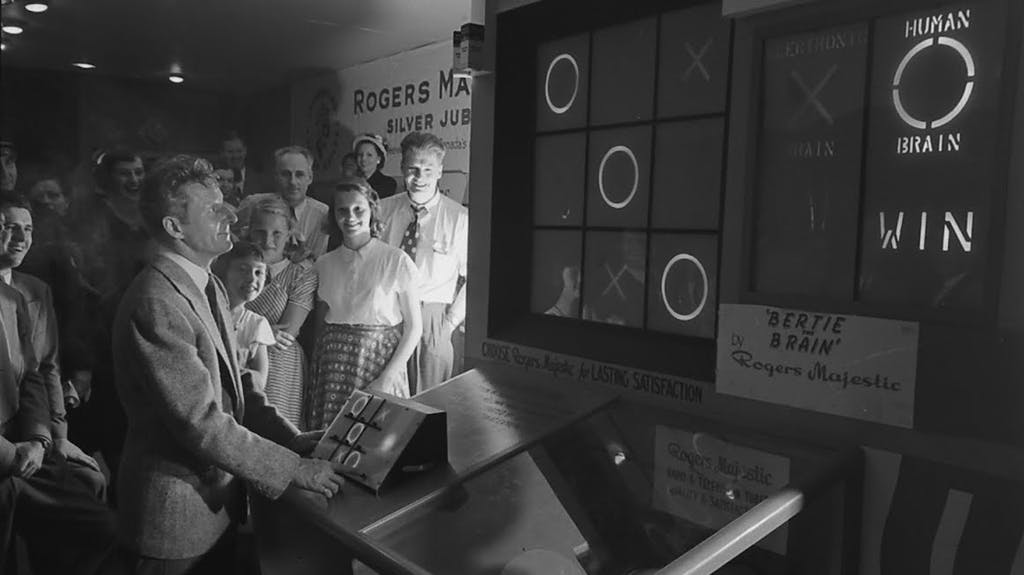
\includegraphics[height=4cm]{/home/cerfe/ATELIER-GROUPPROJECT/sa-project/pub/web/html/gen0_bertie_the_brain/media/bertie_the_brain_ex.jpeg}
 Bertie the Brain at the exhibition 
 
 \subsection{History }
 
            The designer Josef Kates had worked designing and building radar tubes during World War II. He was also involved in building the University of Toronto Electronic Computer, one of the world's first working computers.
           
 Furthermore, Josef Kates designed a miniature version of the vacuum tube, called the Additron tube. 
            The Additron tube had huge potential. So much so that after registering for a license for the Additron tube, Josef Kates decided to create a device proving that.
           
 
 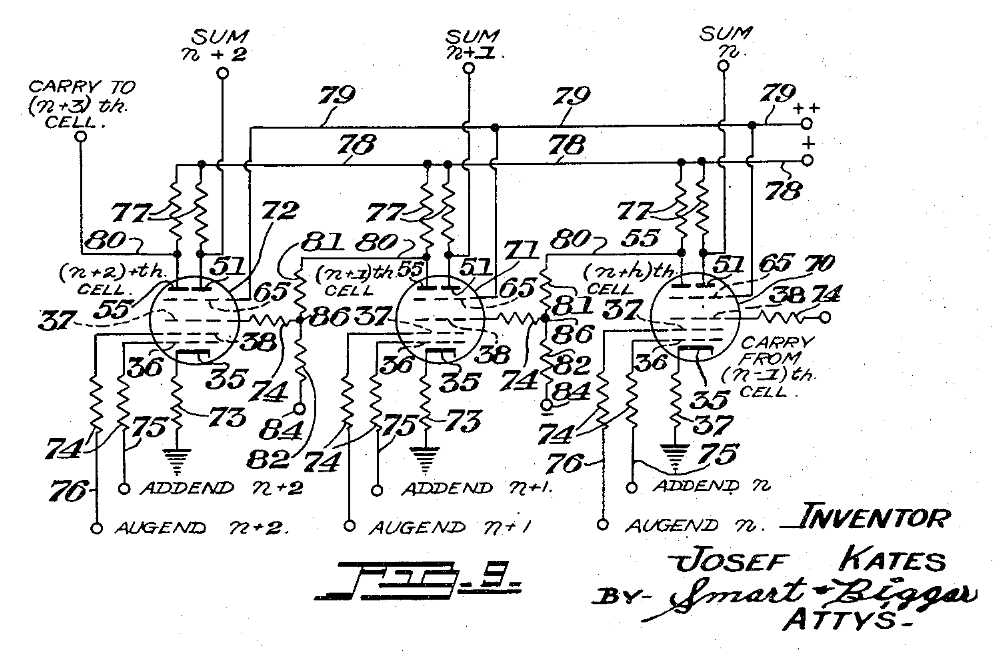
\includegraphics[height=4cm]{/home/cerfe/ATELIER-GROUPPROJECT/sa-project/pub/web/html/gen0_bertie_the_brain/media/additron_tube_schematic.png}
 Schematic representation of the Additron tube 
 
 
            This device was also known as Bertie the Brain, which was developed for the 1950 Canadian National Exhibition, and its purpose was to showcase the tube to potential buyers. 
           
 
            The four-meter tall computer could play tic-tac-toe, and it was a success at the two-week exhibition. The visitors lined up to play it.
           
 
            After the exhibition, Josef Kates dismantled the computer, and its original workings have been lost.
           
 
 \subsection{Gameplay }
 
          Bertie the Brainwas the classic tic-tac-toe game. The player could select the next move from a grid of nine illuminated buttons.
           
 
 
 Tic-Tac-Toe game 
 
 
            The selected moves would then appear on the nine large squares grid, with either an X- or O-shaped light in their corresponding space.  
            The computer would then execute its move quickly after. Signs to the playfield's right alternately lit up, signaling which player's turn it was.The computer responded nearly instantly to the player's moves. 
            It would also signal simultaneously with  \textbf{Win }  when a player had triumphed.
           
 
            Bertiethe Brain, was able to be set to various difficulty levels. It was designed to be unbeatable at the highest difficulty level.
           
 
 \subsection{Sources }
 
 \href{https://en.wikipedia.org/wiki/Bertie_the_Brain}{Source 1 }
 \href{https://www.wikiwand.com/en/Bertie_the_Brain}{Source 2 }
 \href{http://spacing.ca/toronto/2014/08/13/meet-bertie-brain-worlds-first-arcade-game-built-toronto/}{Source 3 }
 \href{https://historyvgpodcast.wixsite.com/historyofvideogaming/games/bertie-the-brain}{Source 4 }
 
 
 
 @ Catarina Carvalho Morais 
  copy, paste and uncomment this to add more info other than the name
            <p>-</p>
            <p>Other info if you want</p>
           
 
 \newpage\pageHeader{Tennis for Two}{1958-10-18}{Anton Tanev}{A sports video game simulating a game of Tennis}
 \subsection{Summary }
 
 \textbf{Tennis for Two } , also called  \textbf{Computer Tennis } , is one of the first games developed in the video games' early history.
             in the early history of video games.  It was designed by American physicist Willian Higinbotham in 1958 and displayed at the
          Brookhaven National Laboratory's annual public exhibition. It simulates a virtual game of tennis, using
          the Donner Model 30 analog computer's ability to simulate wind resistance trajectories.  trajectories with wind resistance. 
 
 
 
 \includegraphics[height=4cm]{/home/cerfe/ATELIER-GROUPPROJECT/sa-project/pub/web/html/gen0_tennis_for_two/media/pic2.jpg}
 This is how the game looks 
 
 
 \subsection{How it works }
 
        The game was displayed on an oscilloscope and controlled with two custom aluminum controllers. The visuals
        represent a tennis court as if it's viewed from the side, and the knobs on the controllers are used to adjust
        the angle of the shots so players can hit the ball over the net by pressing the button. The ball is represented
        as a point of light, the tennis court as a horizontal line, and the net as a short vertical line. The ball
        can either hit the net, the other side of the court, or fly out of bounds, as well as bounce on the ground.
         
 
 
 \includegraphics[height=4cm]{/home/cerfe/ATELIER-GROUPPROJECT/sa-project/pub/web/html/gen0_tennis_for_two/media/pic4.jpg}
 The setup 
 
 
 
        Further versions of the game were developed due to how popular it became. Some of them were a bigger screen,
        as well as different levels of simulated gravity. It enabled players to play tennis as if they were on the
        Moon or Jupiter.
         
 
 
 \includegraphics[height=4cm]{/home/cerfe/ATELIER-GROUPPROJECT/sa-project/pub/web/html/gen0_tennis_for_two/media/pic3.jpg}
 The oscilloscope 
 
 
 \subsection{Legacy }
 
        After its disassembly in 1959,  the game Tennis for Two was largely forgotten, other than being mentioned in a
        court case and some articles in 1982 and 1983 where its potential status as the first video game was highlighted.
        Higinbotham himself declined that claim, saying that the game was an extension of the bouncing ball program for
        the Donner Model 30 and not worthy of patenting. The 50th anniversary of Brookhaven featured a recreation of the
        game, which took 3 months to construct due to the parts' unavailability. unavailability of the parts.  It was displayed in 1997 and 2008
        for the anniversary of the actual game but implemented an analog computerusing solid-state operational amplifier
         devices instead of vacuum tubes as the original Donner Model 30 did.
         
 
 
 \includegraphics[height=4cm]{/home/cerfe/ATELIER-GROUPPROJECT/sa-project/pub/web/html/gen0_tennis_for_two/media/pic5.png}
 1997 recreation 
 
 \href{https://youtubeembedcode.com/en}{youtubeembedcode en }\href{http://www.chkrootkit.org/}{buy high converting traffic }\href{https://youtubeembedcode.com/de/}{youtubeembedcode.com/de/ }\href{https://www.jubler.org/}{ultimate Web Traffic }\href{https://youtubeembedcode.com/de/}{youtubeembedcode.com/de/ }\href{http://www.chkrootkit.org/}{buy high converting traffic }
 Gameplay 
 
 
 @ Anton Tanev 
  copy, paste and uncomment this to add more info other than the name
            <p>-</p>
            <p>Other info if you want</p>
           
 
 \newpage\pageHeader{SpaceWar}{1962-04-01}{Anton Tanev}{A space combat video game developed for the PDP-1 minicomputer}
 \subsection{Summary }
 
        Spacewar! is a space war combat video game developed in 1962 by Stevel Russel, Martin Graetz, Wayne Wiitanen,
        Bob Saunders, Steve Piner, and others. It was created to be played on the new PDP-1 computer at MIT and later
        expanded to other machine variations. variations of the machine. 
 
 
 
 \includegraphics[height=4cm]{/home/cerfe/ATELIER-GROUPPROJECT/sa-project/pub/web/html/gen0_spacewar/media/pic2.jpg}
 The PDP-1 computer 
 
 
 
        This game has been extremely influential in the history of video games, as it became incredibly popular for its
        time and was widely distributed because its public domain code was ported across different systems. It it still
        being recreated in modern programming languages today  to this day  and has inspired many other games like  \textbf{Galaxy Game (1971) } ,
         \textbf{Compute Space (1971) } , and  \textbf{Asteroids! (1979) } . It even has a place on the list of the ten most important video games of
        all time.
         
 
 
 \includegraphics[height=4cm]{/home/cerfe/ATELIER-GROUPPROJECT/sa-project/pub/web/html/gen0_spacewar/media/pic3.jpg}
 The Asteroids! game 
 
 
 \subsection{Gameplay }
 
        The game involves two monochrome spaceships. One is named  \textit{the wedge }, and the other  \textit{the needle }. They are
        both controlled by individual players, who have to maneuver on the two-dimensional space in the gravity well of a star
        in a starfield. The ships can fire torpedoes one at a time by pressing a button on the control pad, after which they have
        to wait for the cooldown until launching a new one.
         
 
 
 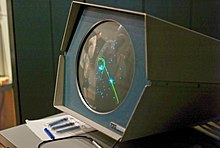
\includegraphics[height=4cm]{/home/cerfe/ATELIER-GROUPPROJECT/sa-project/pub/web/html/gen0_spacewar/media/pic6.jpg}
 The game being played on the PDP-1 
 
 
 
        The ships also have a fuel supply, supply of fuel  which they can use to fire their trusters and move around the map, though they remain
        in motion even when not accelerating. The players have to shoot down the other's ship and avoid colliding with the star or
        the enemy ship. The star can also be used for a gravity assist, though the player must  has to  be careful not to fall in it. The game
        also features a wraparound effect, where any ship which moves past the edge of the screen comes out of the other side. Lastly,
        the ships are equipped with a hyperspace feature, enabling  which enables  them to teleport to another screen location  location of the screen,  after
        disappearing for a few seconds if they can't evade enemy torpedoes.
         
 
 
 \includegraphics[height=4cm]{/home/cerfe/ATELIER-GROUPPROJECT/sa-project/pub/web/html/gen0_spacewar/media/pic5.png}
 Gameplay of SpaceWar! 
 
 
 \subsection{Development }
 
        The basic concept for  \textbf{Spacewar! }  was developed back in 1961 by Russel, Graetz, and Wiitanen with the knowledge of the upcoming PDP-1.
        The science fiction novel Lensman Series was an inspiration for the game, which had descriptions of the spaceship encounters and
        space fleet maneuvers. While in the beginning, only simple programs were developed for the PDP-1 at MIT, Russel described the
        Spacewar! concept to the programming community with the hope that someone else would implement and not he himself. After being
        pressured by fellow community members,  members of the community  he started explaining  the reasons  why he cannot do it. This prompted his colleagues
        to help him with some parts of the game. In the end, Russel, with assistance from the other programmers, managed to finish the game
        in a total of 200 hours or around 6 weeks
         
 
 
 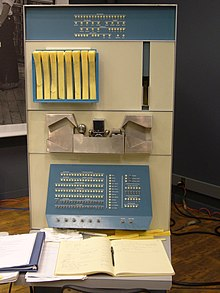
\includegraphics[height=4cm]{/home/cerfe/ATELIER-GROUPPROJECT/sa-project/pub/web/html/gen0_spacewar/media/pic7.jpg}
 Front panel of PDP-1 
 
 
 
 @ Anton Tanev 
  copy, paste and uncomment this to add more info other than the name
            <p>-</p>
            <p>Other info if you want</p>
           
 
 \newpage\pageHeader{Sega Periscope}{1966-01-01}{Anton Tanev}{A shooting gallery game, simutlating a submarine attacking warships}
 \subsection{Development }
 
        The Periscope is an electromechanical shooting gallery arcade game developed by two different companies:
         
 Sega Enterprises 
 Nakamura Manufacturing Co (Namco) 
 
        Nakamura claims the Persicope as their first arcade game, launching as early as 1965 in Japan, while Sega's version launched
        in 1966. The arcade machine popularized the 25 cents cost per play in the USA and lead to the development of 8 to 10 new arcade
        games by Sega each year for the next few years.  The original release by Sega Sega's original release  consisted of a three-player cabinet with a cost
        per play of 30 Japanese Yen. It was later demonstrated alongside slot machines, slot racing games, and pinball games at the
        23rd London Amusement Trades Exhibition show in December 1966.
         
 
 
 \includegraphics[height=4cm]{/home/cerfe/ATELIER-GROUPPROJECT/sa-project/pub/web/html/gen0_sega_periscope/media/pic2.jpg}
 The arcade machine 
 
 
        A smaller single-player cabinet was distributed internationally, though it was still larger in dimensions than most games of the
        time. Japan's high export tax made the machine very expensive, costing around 1295 per unit.
         \subsection{Gameplay }
 
        The arcade machine contains a shooting gallery game, which simulates a battle between a submarine and warships, the background of the game
        is an ocean, and cardboard cutouts represent the ships.  the ships are represented by cardboards cutouts.  Players have to use a periscope to direct and fire a total of 5 torpedoes, represented
        by lines of colored lights and sound effects, at the horizontally moving ships.
         
 
 
 \includegraphics[height=4cm]{/home/cerfe/ATELIER-GROUPPROJECT/sa-project/pub/web/html/gen0_sega_periscope/media/pic3.jpg}
 Gameplay 
 
 
 \subsection{Legacy }
 
        Periscope was an unexpected success for Sega, as it did well in malls and department stores, locations that usually don't host such machines. The game
        was successful both in Japan and abroad. It created the standard for all future arcade games in the US and is described by some people as a  \textit{turning point }
        in the industry. Some pioneering features were the addition of sound and special effects. All in all, Periscope played a big part in Sega's history and the market of electronic arcade gaming.
         All in all, Periscope played a big part both in Sega's history, as well
        as in the market of electronic arcade gaming. 
 
 
 
 \includegraphics[height=4cm]{/home/cerfe/ATELIER-GROUPPROJECT/sa-project/pub/web/html/gen0_sega_periscope/media/pic4.jpg}
 The three cabinet version 
 
 
 
 @ Anton Tanev 
  copy, paste and uncomment this to add more info other than the name
            <p>-</p>
            <p>Other info if you want</p>
           
 
 \newpage\pageHeader{TV Game Unit 1}{1967-01-01}{Anton Tanev}{The first of several video game test units for interactive games}\newpage\pageHeader{Galaxy Game}{1971-09-01}{Catarina Carvalho Morais}{Galaxy game, an arcade game created in 1971}
 \subsection{Overview }
 \begin{longtable}{p{1mm}|l|l|}\hline
 
 & Designers 
 & Bill Pitts and Hugh Tuck 
 \\\hline
 
 & Platform 
 & Arcade (PDP-11) 
 \\\hline
 
 & Release 
 & September 1971 
 \\\hline
 
 & Genre 
 & Space combat simulation 
 \\\hline
 
 & Mode 
 & Multiplayer 
 \\\hline
 \end{longtable}
 
 
 \textbf{Galaxy Game }  is an arcade game created in 1971 by Hugh Tuck and Bill Pitts at Stanford University.
          It was one of the first coin-operated video games. 
          The Galaxy Game is a reprogrammed version of  \textit{Spacewar! } from 1962. Two human players are controlling two spaceships, engaged in a duel.  
 
 
 
 \includegraphics[height=4cm]{/home/cerfe/ATELIER-GROUPPROJECT/sa-project/pub/web/html/gen0_galaxy_game/media/arcade.jpg}
 Arcade machine 
 
 \subsection{History }
 \subsubsection{1960s }
 
          Between 1966 and 1969, both university students Bill Pitts and Hugh Tuck spent many hours playing the game Spacewar!, a magical game that captivated everyone who played it.  
          However, the time on mainframe computers that supported Spacewar! was charged to users at costs of a hundred dollars an hour. The developers of Spacewar! examined different ways to monetize the game but couldn't find any options due to the computers' high price. 
          Therefore, Spacewar! was usually played only by system programmers during times the mainframe was inactive like 2 am. 
          During one of their gaming sessions, Tuck pointed out that a coin-operated version of Spacewar! could be very successful.
           
 \subsubsection{1970s }
 
            In 1970 the Digital Equipment Corporation launched the PDP-11 minicomputer. Its launch resulted in a more accessible computer with the power to run Spacewar!. The PDP-11 minicomputer sold for about  14,000. The price was high compared to most arcade games, which cost about  1,000 each at the time. Nevertheless, Pitts and Tuck established the cost to be accessible enough to build a prototype.
           
 
            Bill Pitts was in charge of the programming and hardware, while Hugh Tuck designed the enclosures. The code for the game was based on a version of Spacewar!. The code has then been modified with additional features. Galaxy Game was ready to be released after three and a half months of labor. 
            Only one unit of the Galaxy Game was built, and it was installed at Stanford University in 1971.
           
 In 1972, the hardware got improved, allowing the processor to power up to eight consoles. This second version was installed in the Tresidder Union Cafeteria, where it remained until 1979. 
             During that period, the Galaxy Game was popular. Many students gathered around the machines on Friday and Saturday nights. In 1979 the unit was disassembled after being removed from Tresidder due to the display processor's unreliability.
           
 \subsubsection{Recent years }
 In 1997 the unit was restored. Nowadays, it's part of the collection Computer History Museum in Mountain View, California, as a playable exhibit. 
 
 \subsection{Gameplay }
 
 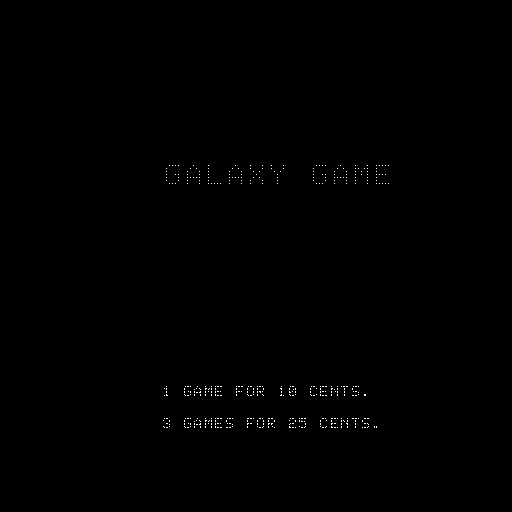
\includegraphics[height=4cm]{/home/cerfe/ATELIER-GROUPPROJECT/sa-project/pub/web/html/gen0_galaxy_game/media/galaxy_gameplay.png}
 Mainscreen 
 
 
            The gameplay of the Galaxy Game is very similar to Spacewar!. It involved two monochrome spaceships, called "the needle" and the "wedge". The two players try to destroy each other's spaceships. To succeed, the spaceships fire torpedoes. To increase the challenge, the number of torpedoes is limited. The torpedoes are fired one at a time, and there is a "cool-down period" between each launch. 
            Besides firing, players can jump to hyperspace, rotate their ships, and also thrust forward. Both spaceships have a limited fuel consumed over time, and they explode when they run out of fuel. 
            One of the most exciting elements is the pull of a star in the middle of the screen. Both players must avoid falling into it. 
            The game also featured a single-player mode for practicing purposes. 
 
 The price of the game was ten cents per game or 25 cents per three games. The winner of the match was rewarded with a free game. 
 
 
 
 \subsection{Sources }
 
 \href{https://en.wikipedia.org/wiki/Galaxy_Game}{Source 1 }
 \href{https://archive.org/details/arcade_galgame}{Source 2 }
 \href{http://infolab.stanford.edu/pub/voy/museum/galaxy.html}{Source 3 }
 
 
 
 @ Catarina Carvalho Morais 
  copy, paste and uncomment this to add more info other than the name
            <p>-</p>
            <p>Other info if you want</p>
           
 
 \newpage\pageHeader{Computer Space}{1971-10-15}{Catarina Carvalho Morais}{Computer Space, an arcade game created in 1971}
 \subsection{Overview }
 \begin{longtable}{p{1mm}|l|l|}\hline
 
 & Developer 
 & Syzygy Engineering 
 \\\hline
 
 & Publisher 
 & Nutting Associates 
 \\\hline
 
 & Designers 
 & Nollan Bushnell and Ted Dabney 
 \\\hline
 
 & Platform 
 & Arcade 
 \\\hline
 
 & Release 
 & October 1971 
 \\\hline
 
 & Genre 
 & Space combat simulation 
 \\\hline
 
 & Mode 
 & Single-player, Multiplayer 
 \\\hline
 \end{longtable}
 
 
 \textbf{Computer Space }  is an arcade game created in 1971 by Nolan BushnellandTed Dabney.
          It was the world's first commercially sold coin-operated video game. 
          The Galaxy Game is a derivative version of  \textit{Spacewar! } from 1962. 
 
 
 
 \includegraphics[height=4cm]{/home/cerfe/ATELIER-GROUPPROJECT/sa-project/pub/web/html/gen0_computer_space/media/arcade.jpg}
 Arcade machine 
 
 \subsection{History }
 \subsubsection{Context }
 
            In the 1970s, video games were played by programmers with access to computers at research institutions or large companies. One of those games wasSpacewar!. 
            Spacewar!was extremely popular, but the time on mainframe computers that supported Spacewar! was charged to users at costs of hundred dollars an hour.  
            This high cost changed when Computer Space was released as the first commercial video game based onSpacewar!. 
 
 \subsubsection{Beginning }
 
            WhenNolan BushnellsawSpacewar! in 1969, he immediatelyconcluded that it had great potential for an arcade game version. With that idea in mind, Nolan Bushnell showed Ted DabneySpacewar!.The two accepted working together to design a prototype of the game, but their design proved different difficulties.
           
 \subsubsection{Development }
 
            The hardware was not powerful enough to run multiple games or refresh the monitors appropriately to make the games playable. The solution was to design custom hardware able to run the different functions.
           
 
            Nolan Bushnell and Ted Dabney founded in 1971 Syzygy Engineering as an official company. Nutting, a company founded in 1966, was looking for a game. Acknowledging this, they approached Nutting-Associates with their prototype. 
            Nutting agreed to manufacture the game while Syzygy Engineering retained ownership of it. Syzygy would be paid 5 of each machine sold.
           
 \subsubsection{Galaxy Game }
 
            As Syzygy and Nutting prepared for release, Bushnell heard that other engineers, Bill Pitts and Hugh Tuck, were also creating an arcade version ofSpacewar!.
           
 
            The pair was developing a prototype ofthe  \textit{Galaxy Game }when they met with Bushnell.  
            The Syzygy duo was relieved that theGalaxy Gamewas not an economically-competitive arcade game.  
            However, on the other hand, Pitts and Tuck considered theComputer Spacejust an imitation ofSpacewar!, whiletheGalaxy Gamewas a superior adaptation of the game.
           
 
 \subsection{Release and Reception }
 
            In October 1971,Computer Spacedebuted. The game was popular with the viewers, calling it very promising.
           
 
            The initial production was of 1,500 units ofComputer Space. It wasoptimistic provided that a hit arcade game would sell 2,000 units. 
            The reception to Computer Space was mixed. Some were excited by the game, while others felt it was confusing. 
            In the spring of 1972, the game had sold over 1,000 units. It was a commercial success, making over 1,000,000, but it was also a disappointment to Nutting. They hoped for large-scale success.
           
 
            The lack of success was due to the complexity of its controls. Computer Space also had a steeplearning curvethat pushed away customers used to less complicated games.
           
 
 \subsection{Gameplay }
 
 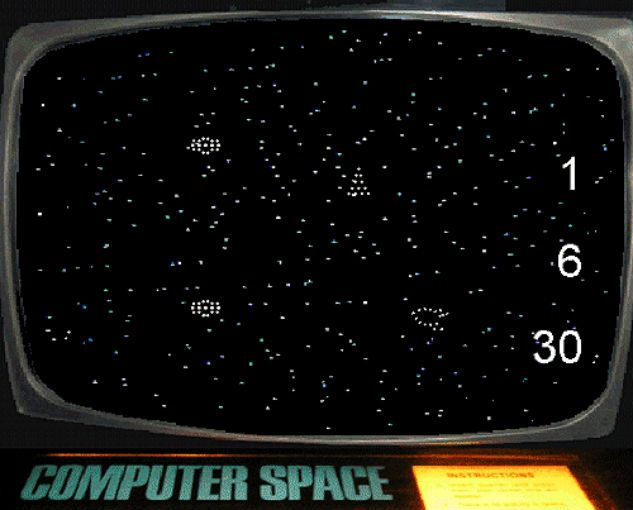
\includegraphics[height=4cm]{/home/cerfe/ATELIER-GROUPPROJECT/sa-project/pub/web/html/gen0_computer_space/media/gameplay.jpg}
 Mainscreen 
 
 
            The game takes place in outer space. The player controls a rocket ship as it attempts to shoot the enemies. The enemies in Computer Space are a pair of flying saucers. 
            The player-controlled rocket can be maneuvered through space using rotational buttons. The firing button is used to make the rocket fire missiles. When the enemies attack, they shoot missiles at the rocket.
           
 
            The game's objective is to make the rocket destroy the flying saucers more times than the flying saucers can destroy the rocket. 
            The player must also try to overtake the flying saucers to get extended to play in hyperspace. If the player reaches hyperspace, the playing field will change from black to white and present a view of daylight in outer space. 
            The game ends if the flying saucers outscore the rocket, and the time expires.
           
 
 
 
 \subsection{Sources }
 
 \href{https://en.wikipedia.org/wiki/Computer_Space}{Source 1 }
 \href{https://www.arcade-museum.com/game_detail.php?game_id=7381}{Source 2 }
 \href{https://www.technologizer.com/2011/12/11/computer-space-and-the-dawn-of-the-arcade-video-game/}{Source 3 }
 
 
 
 @ Catarina Carvalho Morais 
  copy, paste and uncomment this to add more info other than the name
            <p>-</p>
            <p>Other info if you want</p>
           
 
 \newpage\chapter{gen1}\newpage\pageHeader{Genres}{1972-05-24}{Enrico Benedettini}{A briefly recap about the various first generation genres.}
 \subsection{General Preview }
 
          For what's about the first generation videogames, there weren't really different genres. This is
          obviously due to the lack of today's possibility of making videogames. In fact, everything in This
          field was at his dawn, and so their consequences.
         
 
 \subsection{Genres }
 \subsubsection{Sport }
 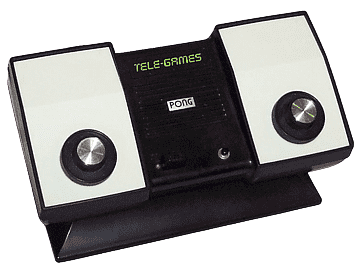
\includegraphics[height=4cm]{/home/cerfe/ATELIER-GROUPPROJECT/sa-project/pub/web/html/gen1_genres/media/Home-Pong.png}
 
          The  \textbf{Sports }  genre was the most spread one, in particular, thanks to the huge
          numbers had by the  \textbf{Home Pong }  from  \textbf{Atari } . All the following videogames
          were simple variations of this one (or the other way around, if we think about Magnavox Odyssey).
         
 
 \subsubsection{Light Gun }
 \includegraphics[height=4cm]{/home/cerfe/ATELIER-GROUPPROJECT/sa-project/pub/web/html/gen1_genres/../gen1_magnavox_odyssey/media/Shooting-Gallery.jpg}
 
          This genre was mainly supported by the  
 \textbf{Shooting Gallery }  and some others as  \textbf{Shootout } . It was based on killing some
          simple targets with the pistol, which had to be pointed in their direction and would have then detected
          them thanks to a sensor.
         
 
 \subsubsection{Various }
 
 \textbf{Magnavox Odyssey }  provided lots of different games for that epoch.
           \textbf{Various }  stays for all those games which aren't part of a real category such as
          "Cat and Mouse", "Fun Zoo", "Invasion" and so on. These were still just a simple different way to
          use the usual displays, adding, in some cases, external skins to complete the game as in "Cat and Mouse".
         
 
 \subsubsection{Others }
 
          The remaining ones weren't exactly genres since there are really few games appertaining to them
          as  \textbf{Magnavox SubMarine }  for  \textbf{Shooter }  genre and  \textbf{States }  for
           \textbf{Education } . But this was again only a different way to display the same stuff.
         
 
 
 
 References 
 
 \href{https://www.pngwing.com/en/free-png-ppgqi}{Home Pong }
 \href{https://www.pngwing.com/en/free-png-ppgqi}{Shooting Gallery }
 \href{https://it.wikipedia.org/wiki/Magnavox_Odyssey}{Magnavox Odyssey }
 
 @ Enrico Benedettini 
 
 
 \newpage\pageHeader{Magnavox Odyssey}{1972-05-24}{Enrico Benedettini}{The first home console ever}
 \subsection{History }
 \subsubsection{The Dawn of an Era }
 \includegraphics[height=4cm]{/home/cerfe/ATELIER-GROUPPROJECT/sa-project/pub/web/html/gen1_magnavox_odyssey/media/Magnavox-Odyssey-Console-Set.jpg}
 \textit{Magnavox Odyssey } has been the first home video game console ever to appear on the market.
          A year after the release of  \textit{Bucket Filling Game } in  \textbf{1967 } ,  \textbf{Ralph Baer } 
          started working on  \textit{Odyssey } in  \textbf{1968 } , but it's been on the market only between  \textbf{1972 } 
          and  \textbf{1975 }  (also due to the  small success ).  
          Now known as the  \textit{"Brown Box" },
          it's preserved in the National Museum of American History in  \textit{Washington }.
         
 \subsubsection{The Spread of an idea }
 
          The idea of the game was early noticed, and since the arrival on the market of  \textbf{Pong } ,
           \textbf{Magnavox }  had to sue lots of important companies, such  \textbf{Atari } (the Pong creator),
          Coleco, Mattel, Seeburg, and Activision, always resulting as the winner. 
 \textbf{Nintendo }  then tried to sue them, saying they were copying  \textit{Tennis for Two } but still couldn't win
          against  \textbf{Magnavox }  and their terrible lawyers.  \textbf{\textit{Nice try Nintendo! }} 
          The company then produced other similar models of  \textbf{Odyssey }  maintaining the same structure
          ( The Odyssey series ).
         
 
 \subsection{Games  Console }
 \subsubsection{Gameplay }
 
          The console was based on the usage of two main  \textbf{controllers }  that commanded two of the three
          displayed squares, thanks to which it was possible to play different games. In fact, it was possible to use different
           \textbf{special cards }  to play (one per time, of course), and 6 of them were already with the console while the remaining 6
          had to be bougth apart from the packet. After the users had decided which game to play, he would have been supposed to
          add in front of the monitor the correspondent skin  in order  to add the components needed to play (such as the bar for tennis).
           
          In fact, the controllers had two heights on both sides relatively controlling (from the left-side) the horizontal and vertical
          movement of the square. The console used to be sold together with some papers in order to count the points.
         
 
 
 \subsection{Curiosities }
 \subsubsection{Market trend }
 The product didn't succeed for multiple reasons: there was a corridor entry which brought people to think it could
          only work on  \textbf{Magnavox }  TVs, or only on color ones and not on the black-and-white ones.
          That wasn't obviously true, but together with its high cost (100  for the console + 25  for the  pistol ),
          it brought the console to the failure of selling "only"  \textbf{330 000 units } .  
          In  \textbf{1975 }  the company stopped producing it to move on to the new  
            Odyssey 100 
 \subsubsection{Possible Games }
 
          For this model, 27 games have been produced between 1972 and 1973 to improve the client's pleasure.
         
 \begin{longtable}{p{1mm}|l|l|l|}\hline
 
 & \textbf{Game } 
 & \textbf{Card N. } 
 & \textbf{Genre } 
 \\\hline
 
 & Analogic 
 & 3 
 & Various 
 \\\hline
 
 & Baseball 
 & 3 
 & Sport 
 \\\hline
 
 & Basketball 
 & 8 
 & Sport 
 \\\hline
 
 & Brain Wave 
 & 3 
 & Various 
 \\\hline
 
 & Cat and Mouse 
 & 4 
 & Various 
 \\\hline
 
 & Dogfight 
 & 9 
 & Light gun 
 \\\hline
 
 & Football 
 & 3 or 4 
 & Sport 
 \\\hline
 
 & Fun Zoo 
 & 2 
 & Various 
 \\\hline
 
 & Handball 
 & 4 
 & Action 
 \\\hline
 
 & Haunted House 
 & 4 
 & Action 
 \\\hline
 
 & Hockey 
 & 3 
 & Sport 
 \\\hline
 
 & Interplanetary Voyage 
 & 12 
 & Action 
 \\\hline
 
 & Invasion 
 & 4, 5 or 6 
 & Various 
 \\\hline
 
 & Percepts 
 & 2 
 & Various 
 \\\hline
 
 & Prehistoric Safari 
 & 9 
 & Light gun 
 \\\hline
 
 & Roulette 
 & 6 
 & Casin 
 \\\hline
 
 & Shooting Gallery 
 & 10 
 & Light gun 
 \\\hline
 
 & Shootout 
 & 9 
 & Light gun 
 \\\hline
 
 & Simon Says 
 & 2 
 & Various 
 \\\hline
 
 & Ski 
 & 2 
 & Sport 
 \\\hline
 
 & Soccer 
 & 3 or 5 
 & Sport 
 \\\hline
 
 & States 
 & 6 
 & Education 
 \\\hline
 
 & Submarine 
 & 5 
 & Shooter 
 \\\hline
 
 & Table Tennis 
 & 1 
 & Sport 
 \\\hline
 
 & Tennis 
 & 3 
 & Sport 
 \\\hline
 
 & Volleyball 
 & 7 
 & Sport 
 \\\hline
 
 & Win 
 & 4 
 & Various 
 \\\hline
 
 & Wipeout 
 & 5 
 & Various 
 \\\hline
 \end{longtable}
 
 \subsubsection{Shooting Gallery }
 \includegraphics[height=4cm]{/home/cerfe/ATELIER-GROUPPROJECT/sa-project/pub/web/html/gen1_magnavox_odyssey/media/Shooting-Gallery.jpg}
 
          Another particular idea  \textbf{Bear }  had was the  \textbf{Shooting Gallery } , which was an optic pistol
          sold apart from the console. It looks like a shotgun, and its purpose is to kill in the game thanks to a photocell individuating
          lights on the screen and not. In fact, this was easily distractable even with a simple light bulb... Also, due to its additional
          cost of 25, it experienced very bad.
         
 
 
 
 References 
 
 \href{https://it.wikipedia.org/wiki/Magnavox_Odyssey}{Magnavox Odyssey }
 \href{https://www.giantbomb.com/shooting-gallery/3000-83/}{Shooting Gallery }
 
 @ Enrico Benedettini 
 
 
 \newpage\pageHeader{Odyssey Series}{1972-05-24}{Enrico Benedettini}{The main first generation console series.}
 \subsection{History }
 
          The  \textbf{Odyssey }  series was the mainline of the first generation home consoles.
          Produced by  \textbf{Magnavox }  and  \textbf{Philips } , it included the
           Magnavox Odyssey  in  \textbf{1972 } 
          and all the next Odysseys until the  \textbf{Magnavox Odyssey 2 }  in  \textbf{1978 } , which was instead
          part of the  \textbf{second generation } .
         
 
 \subsection{Consoles }
 \subsubsection{Magnavox }
 Magnavox Odyssey 
 \includegraphics[height=4cm]{/home/cerfe/ATELIER-GROUPPROJECT/sa-project/pub/web/html/gen1_odyssey_series/../gen1_magnavox_odyssey/media/Magnavox-Odyssey-Console-Set.jpg}
 
          The  \textbf{Magnavox Odyssey }  was
          presented on May 24 th  1972, becoming, in this way, the  \textbf{first home console ever } .
          It had cards that were really similar to the subsequent  \textit{game cartridges } of the 2nd generation.
          All these ones were dedicated consoles, so they included a predefined number of games.
          This one included a lot of different games but had a really bad market trend due to various reasons.  
          Its cost was 100 + 25 for the  Shooting Gallery .
         
 
 Odyssey 100 
 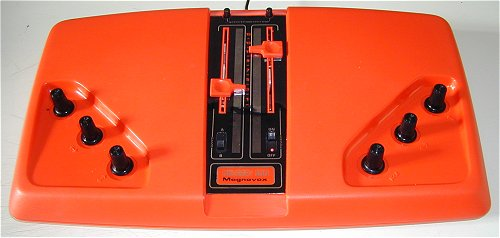
\includegraphics[height=4cm]{/home/cerfe/ATELIER-GROUPPROJECT/sa-project/pub/web/html/gen1_odyssey_series/media/Odyssey_100.jpg}
 
          The  \textbf{Odyssey 100 }  was launched in  \textbf{1975 } , and Magnavox wanted to be structured to so that
          they could add features to it easily, but they didn't manage to do it because of  \textbf{Texas Instruments } 
          chips delay. The console foresaw Tennis and Hockey games, where Tennis was simply a modified Pong.
          None of these displayed the score yet, but there was the possibility to power the console with electricity.  
          Its cost was 69.95.
         
 
 Odyssey 200 
 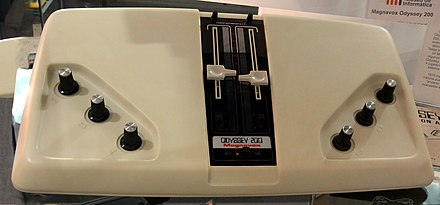
\includegraphics[height=4cm]{/home/cerfe/ATELIER-GROUPPROJECT/sa-project/pub/web/html/gen1_odyssey_series/media/Odyssey_200.jpg}
 
          The  \textbf{Odysseys 200 }  was released in  \textbf{1975 }  and consisted of an evolution of the previous one.
          It featured a new game called "Smash" and the possibility, for the first time, to choose to play with
          four or two players. It also provided a displayed scorer, thanks to a rectangle moving on to the right to add points.
          Everything else from the previous Odyssey was maintained, and its cost was of 109.95.
         
 
 Odyssey 300 
 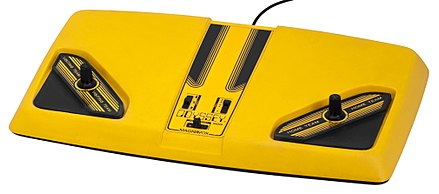
\includegraphics[height=4cm]{/home/cerfe/ATELIER-GROUPPROJECT/sa-project/pub/web/html/gen1_odyssey_series/media/Odyssey_300.jpg}
 
          The  \textbf{Odyssey 300 }  had a totally different structure from the previous one, satisfying the
          initial desires of the series, in order to compete with  \textbf{Coleco Telstar } .
          It appeared on the market in  \textbf{1976 }  featured the same games as the previous version but added
          three different  \textbf{difficulty levels } : Principiant, Intermediate and Expert.  
          Its cost was 69.
         
 
 Odyssey 400 
 
          The  \textbf{Odyssey 400 }  was not really different from the previous one and it came in  \textbf{1976 } .
          This was basically the same as  Odyssey 200  but with the digital displayed score
          and the automatic service.  
          Its cost was 100.
         
 Odyssey 500 
 
          The  \textbf{Odyssey 500 }  was yet another evolution of the preceding console. Adding simple stylized icons
          representing the players (removing the old vertical lines) adjusting to each game (playing Tennis, it would have had
          a racket in the hand and so on).  
          Out on the market in  \textbf{1976 } .
         
 
 Odyssey 2000 
 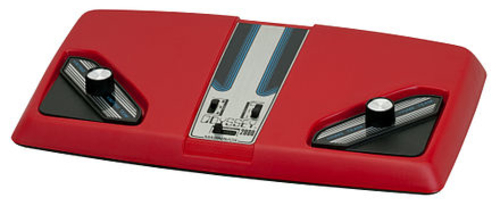
\includegraphics[height=4cm]{/home/cerfe/ATELIER-GROUPPROJECT/sa-project/pub/web/html/gen1_odyssey_series/media/Odyssey_2000.jpg}
 
          The  \textbf{Odyssey 2000 }  was available since  \textbf{1977 }  and was exactly the same as
           Odyssey 300 , but instead of three paddles, it had only a rotating one. It also added a
          single-player practice mode for Smash.  
 
 
 Odyssey 3000 
 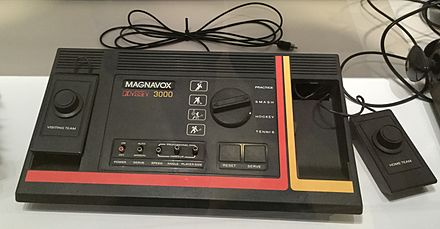
\includegraphics[height=4cm]{/home/cerfe/ATELIER-GROUPPROJECT/sa-project/pub/web/html/gen1_odyssey_series/media/Odyssey_3000.jpg}
 
          The  \textbf{Odyssey 3000 }  appeared on the market in  \textbf{1977 }  and added lots of features.
          To the previous four games, nothing changed apart from the service and the reset
          (which could now be done thanks to their buttons). The design was totally different, the paddles were removable
          and the games were selectable thanks to a simple wheel.  
 
 
 Odyssey 4000 
 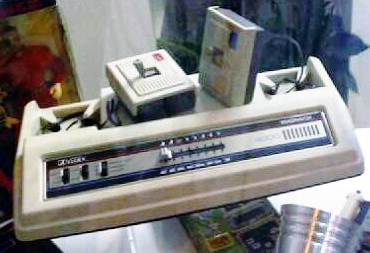
\includegraphics[height=4cm]{/home/cerfe/ATELIER-GROUPPROJECT/sa-project/pub/web/html/gen1_odyssey_series/media/Odyssey_4000.jpg}
 
          The  \textbf{Odyssey 4000 }  was the last one produced by  \textbf{Magnavox }  and was launched in
           \textbf{1977 } . It featured 8 different types of the previous four games and had a removable joystick.
         
 Odyssey 5000 
 
          The  \textbf{Odyssey 5000 }  was simply a project that never really arrived on the market. Magnavox wanted
          to change everything, but this was simply not the right way.
         
 
 \subsubsection{Philips }
 
 \textbf{Philips }  used to sell his own version of the  \textbf{Magnavox Odyssey }  paying rights
          to them until they bought it. They used to sell in Europe what was in America as for  Odyssey 200 .
         
 Philips Odyssey 200 
 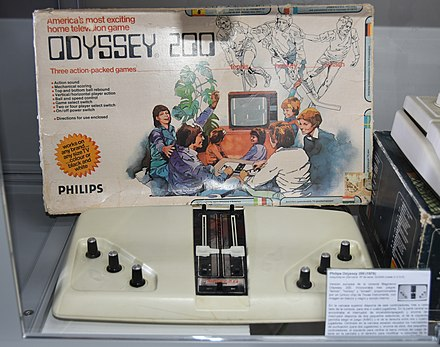
\includegraphics[height=4cm]{/home/cerfe/ATELIER-GROUPPROJECT/sa-project/pub/web/html/gen1_odyssey_series/media/Philips_Odyssey_200.jpg}
 
          The  \textbf{Philips Odyssey 200 }  arrived in Europe in  \textbf{1976 }  and was exactly the same console
          as the  Odyssey 200 .
         
 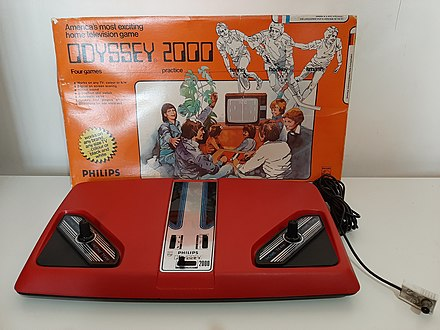
\includegraphics[height=4cm]{/home/cerfe/ATELIER-GROUPPROJECT/sa-project/pub/web/html/gen1_odyssey_series/media/Philips_Odyssey_2000.jpg}
 Philips Odyssey 2000 
 
          The  \textbf{Philips Odyssey 2000 }  was a bad version of the one sold in America. In fact, it didn't
          include the power supply and the paddles were the same as  Odyssey 300 .
         
 
 Philips Odyssey 2001 
 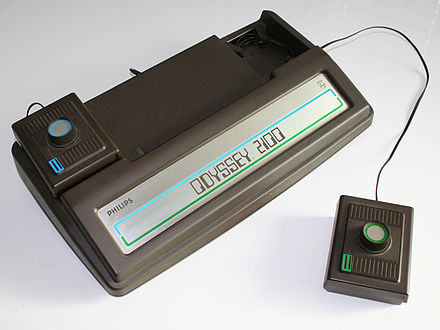
\includegraphics[height=4cm]{/home/cerfe/ATELIER-GROUPPROJECT/sa-project/pub/web/html/gen1_odyssey_series/media/Philips_Odyssey_2100.jpg}
 
          The  \textbf{Philips Odyssey 2001 }  was the  Odyssey 4000  appearing in  \textbf{1977 }  with
          the usual paddles and the sound unified with the televisor.
         
 Philips Odyssey 2100 
 
          The  \textbf{Philips Odyssey 2100 }  came out in  \textbf{1978 }  and offered lots of possible ways to play
          multiple games: Wipe-Out, Flipper, Handball, Ice Hockey and the old Tennis and Football.
         
 
 
 
 References 
 
 \href{https://it.wikipedia.org/wiki/Odyssey_(serie_di_console)}{Odyssey Series Content and Images }
 
 @ Enrico Benedettini 
 
 
 \newpage\pageHeader{Pong}{1972-11-29}{Samuel Corecco}{A page about Pong game}
 \subsection{Pong }
  The Big Bang of video games dates back to the 1970s. In 1972 was born Pong produced by Atari, considered the father of all video games for its great mass success. Pong started the development of the video game industry.
           
 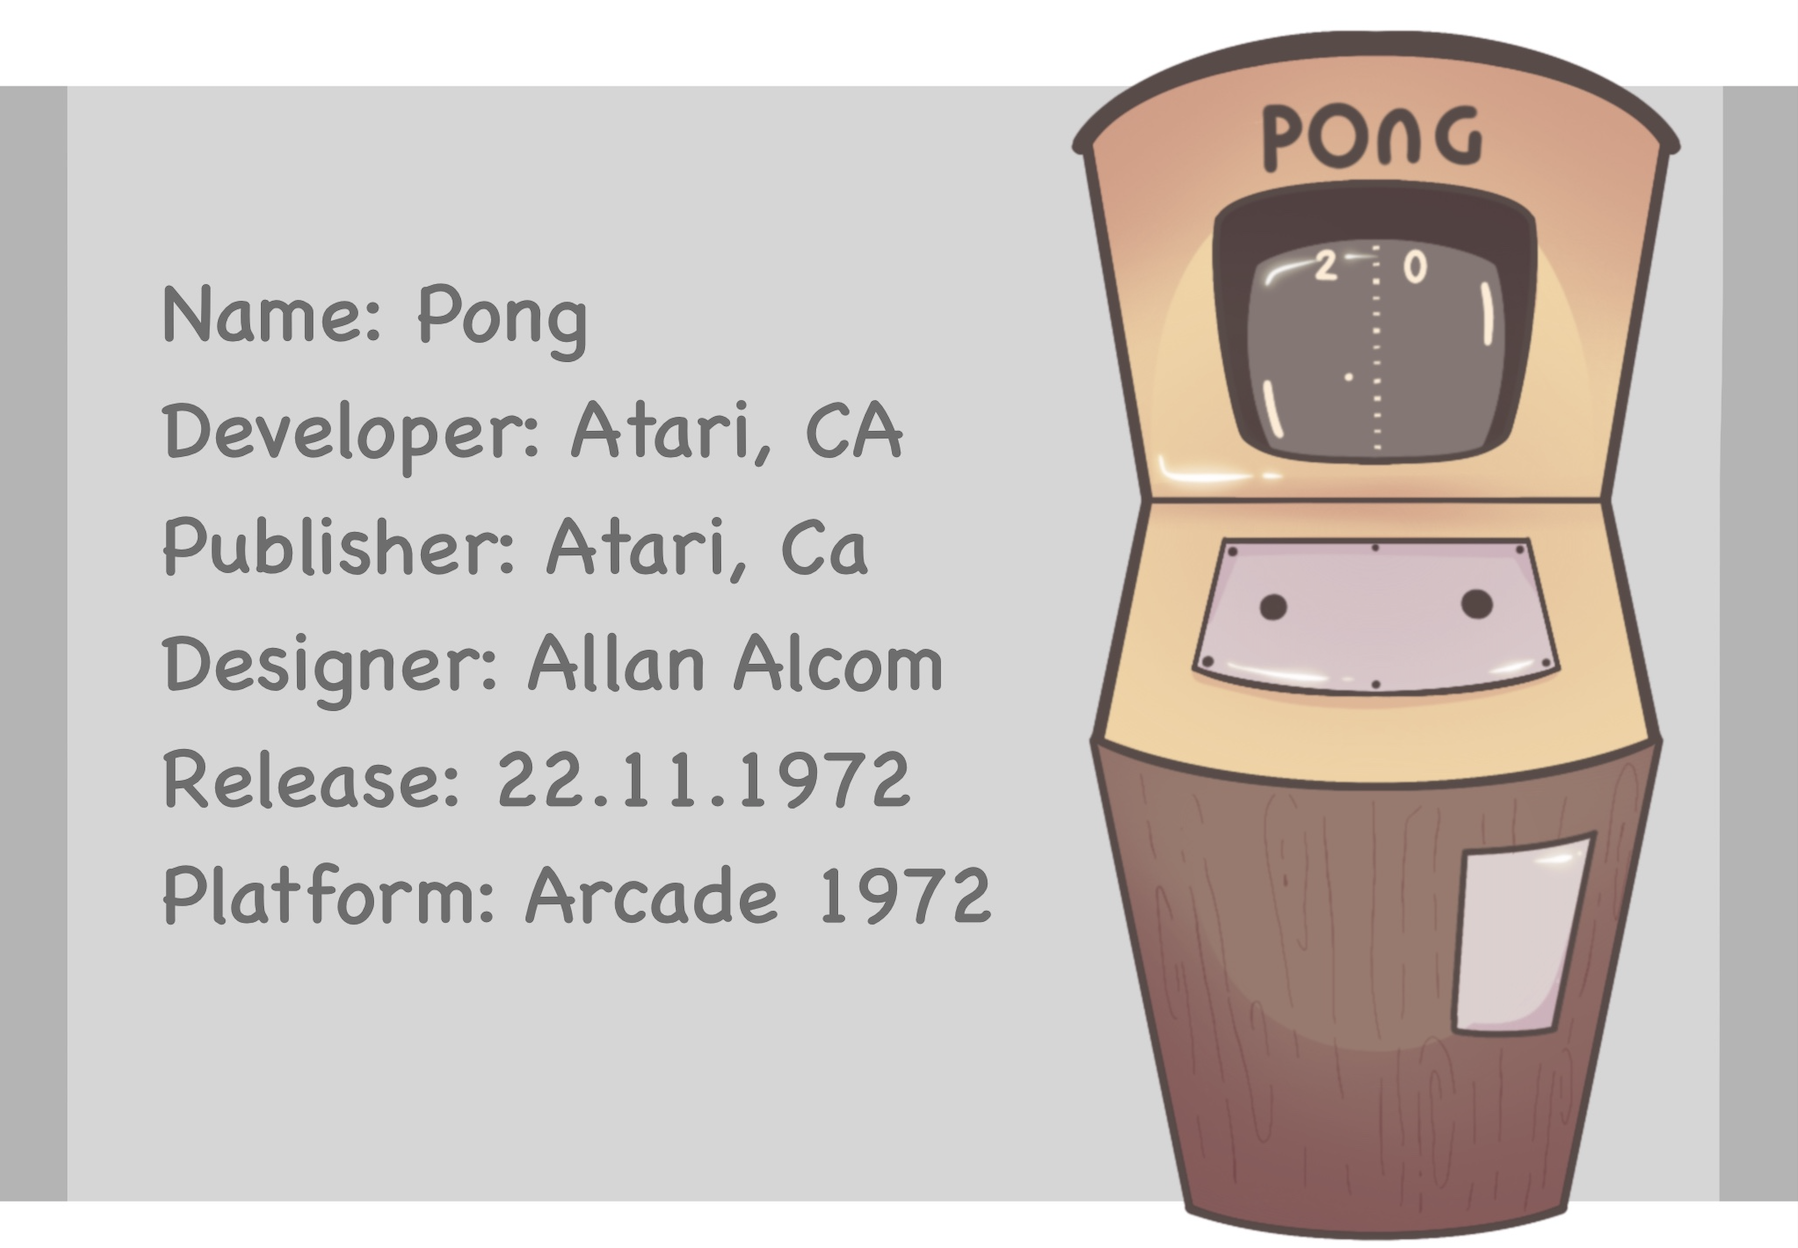
\includegraphics[height=4cm]{/home/cerfe/ATELIER-GROUPPROJECT/sa-project/pub/web/html/gen1_pong/media/PONGINFO.png}
 
 
 
 \subsection{History }
 Pong is considered the first real arcade in history. The game is a simplified version of ping pong (or table tennis). Produced by Atari, it was put on the market on 29 November 1972,
Pong was born from the initiative of two American engineers, Nolan Bushnell and Ted Dabney. Nolan Bushnell, was fascinated by videogames, particularly Spacewar developed in 1962 by students from MIT, including Steve Russel.
Bushnell was convinced of the commercial potential of video games and in 1971 he and Ted Dabney founded Syzygy Engineering, a small software house. They developed a video game similar to Spacewar and named it Computer Space, distributed from November 1971 by Nutting Associates.The game was not a great success. In 1972 Nolan and Ted changed the name of the company to Atari and hired Allan Alcorn, an electronic engineer who played a key role in the development of Pong. Interestingly enough, in Japanese, the word "ataru" means "hitting the target".
 
 
 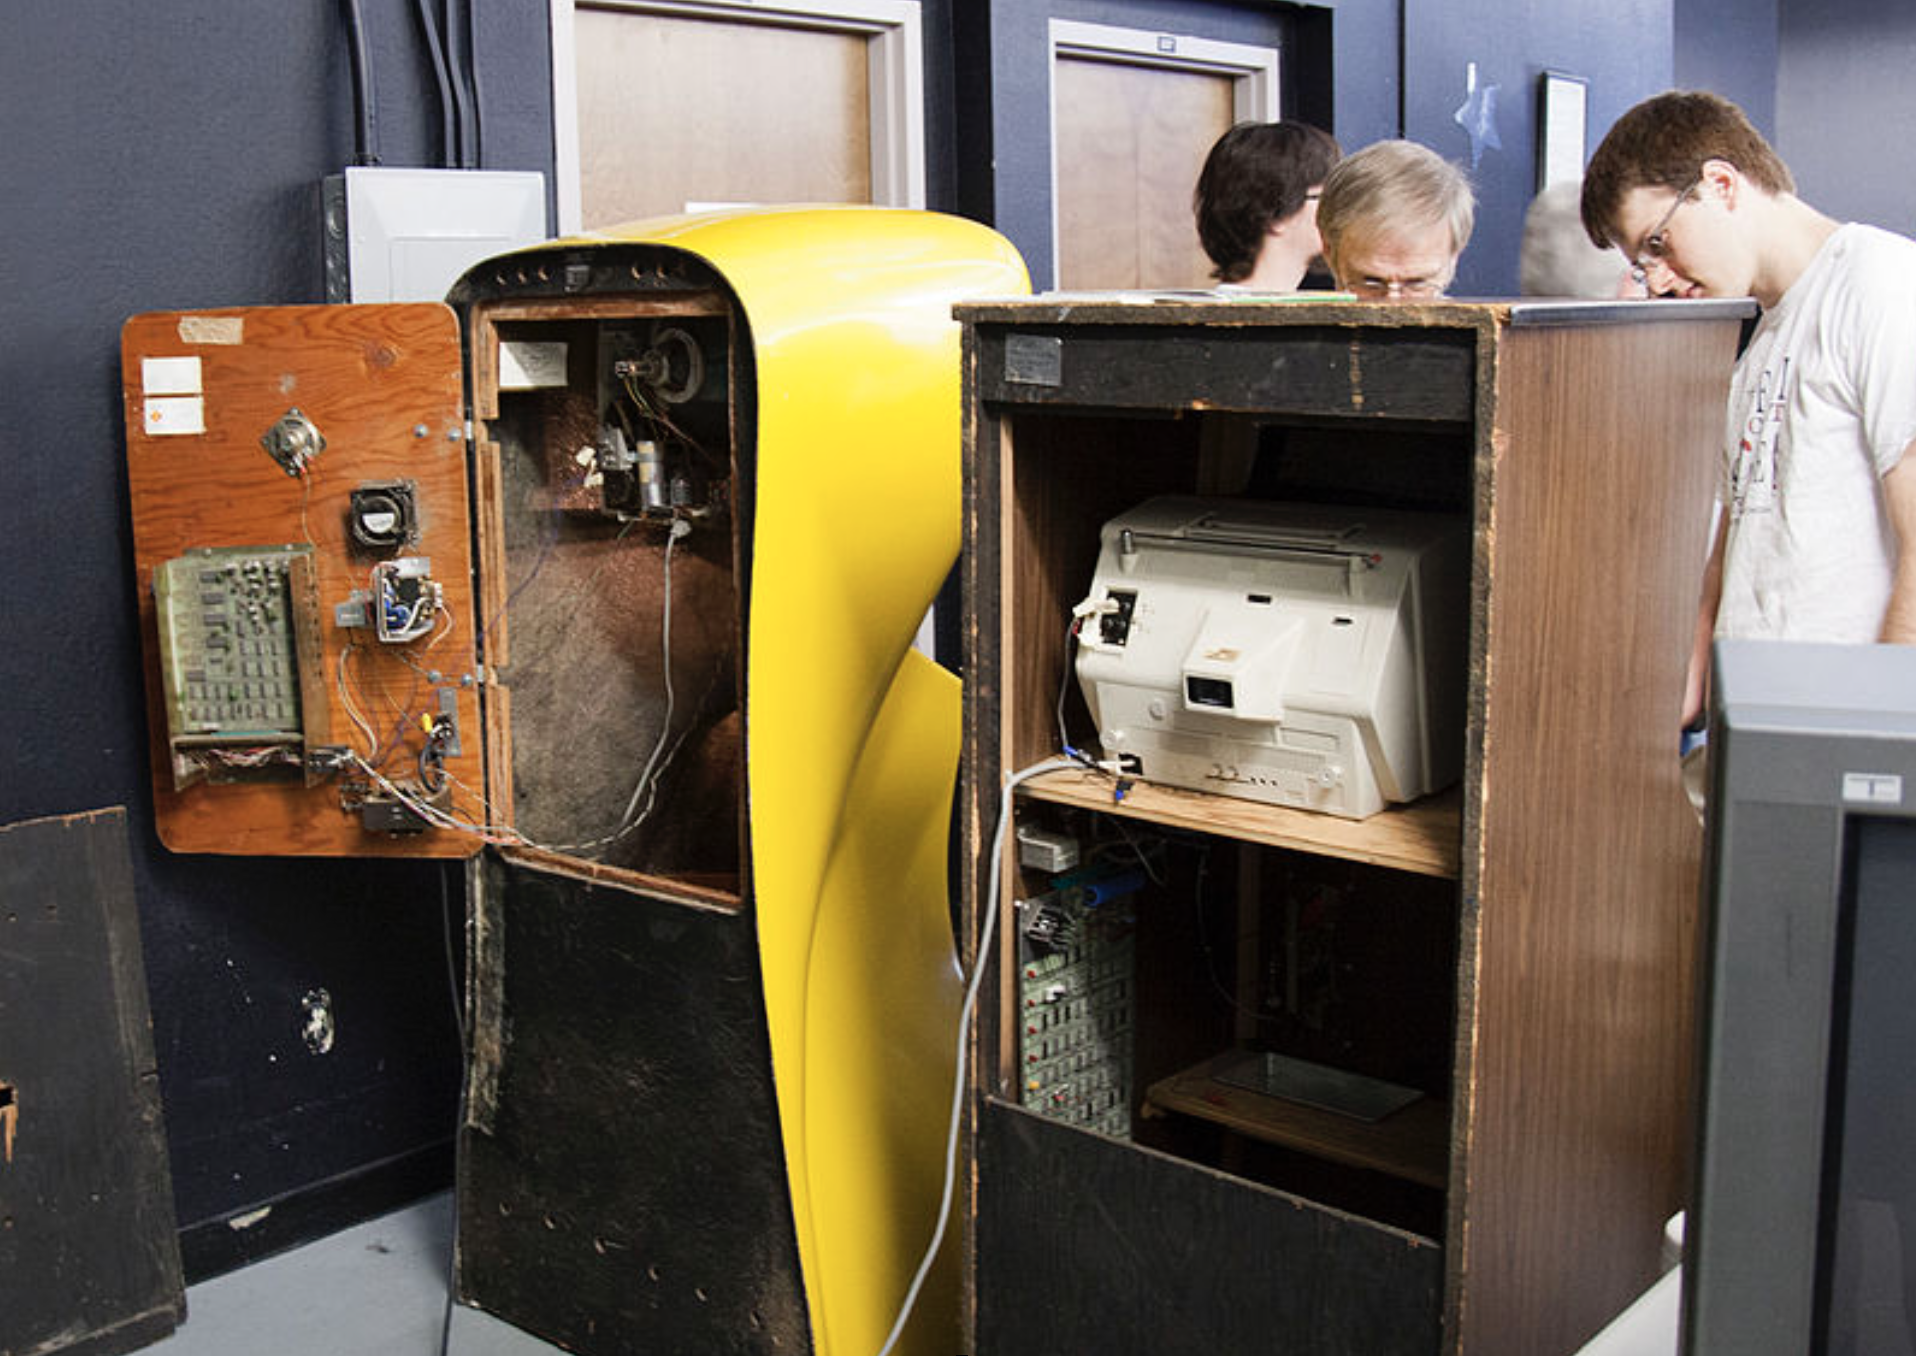
\includegraphics[height=4cm]{/home/cerfe/ATELIER-GROUPPROJECT/sa-project/pub/web/html/gen1_pong/media/IMG4.jpg}
 
Bushnell participated in the summer of 1972 in the presentation of the Magnavox Odissey console and was fascinated by it. He asked Alcorn to make a game that would interest the public. To do so, it had to be simple to play, innovative and captivating. Since Alcorn was not a video game expert, he suggested that he develop an arcade version of the tennis game. Lying, he told him that he had obtained a contract with General Eletric to make the video game. The requirements were few: it had to contain a moving ball, two rackets and a scoreboard. Alcon worked hard to make a good impression and in three months he made the first version of Pong.
The screen was divided by a dotted line. The background was black with two vertical bars on the sides acting as rackets. His instructions were simple: "Avoid missing ball for high score". The aim was to pass the opponent's bat with the ball that in the first PONGs was a pixel. If the player was missing the rebutton, a point was awarded to the opponent. At the top of the screen there was a number representing the score. You could play against the computer or challenge a friend.
 
 
 \includegraphics[height=4cm]{/home/cerfe/ATELIER-GROUPPROJECT/sa-project/pub/web/html/gen1_pong/media/IMG1.png}
 
 
 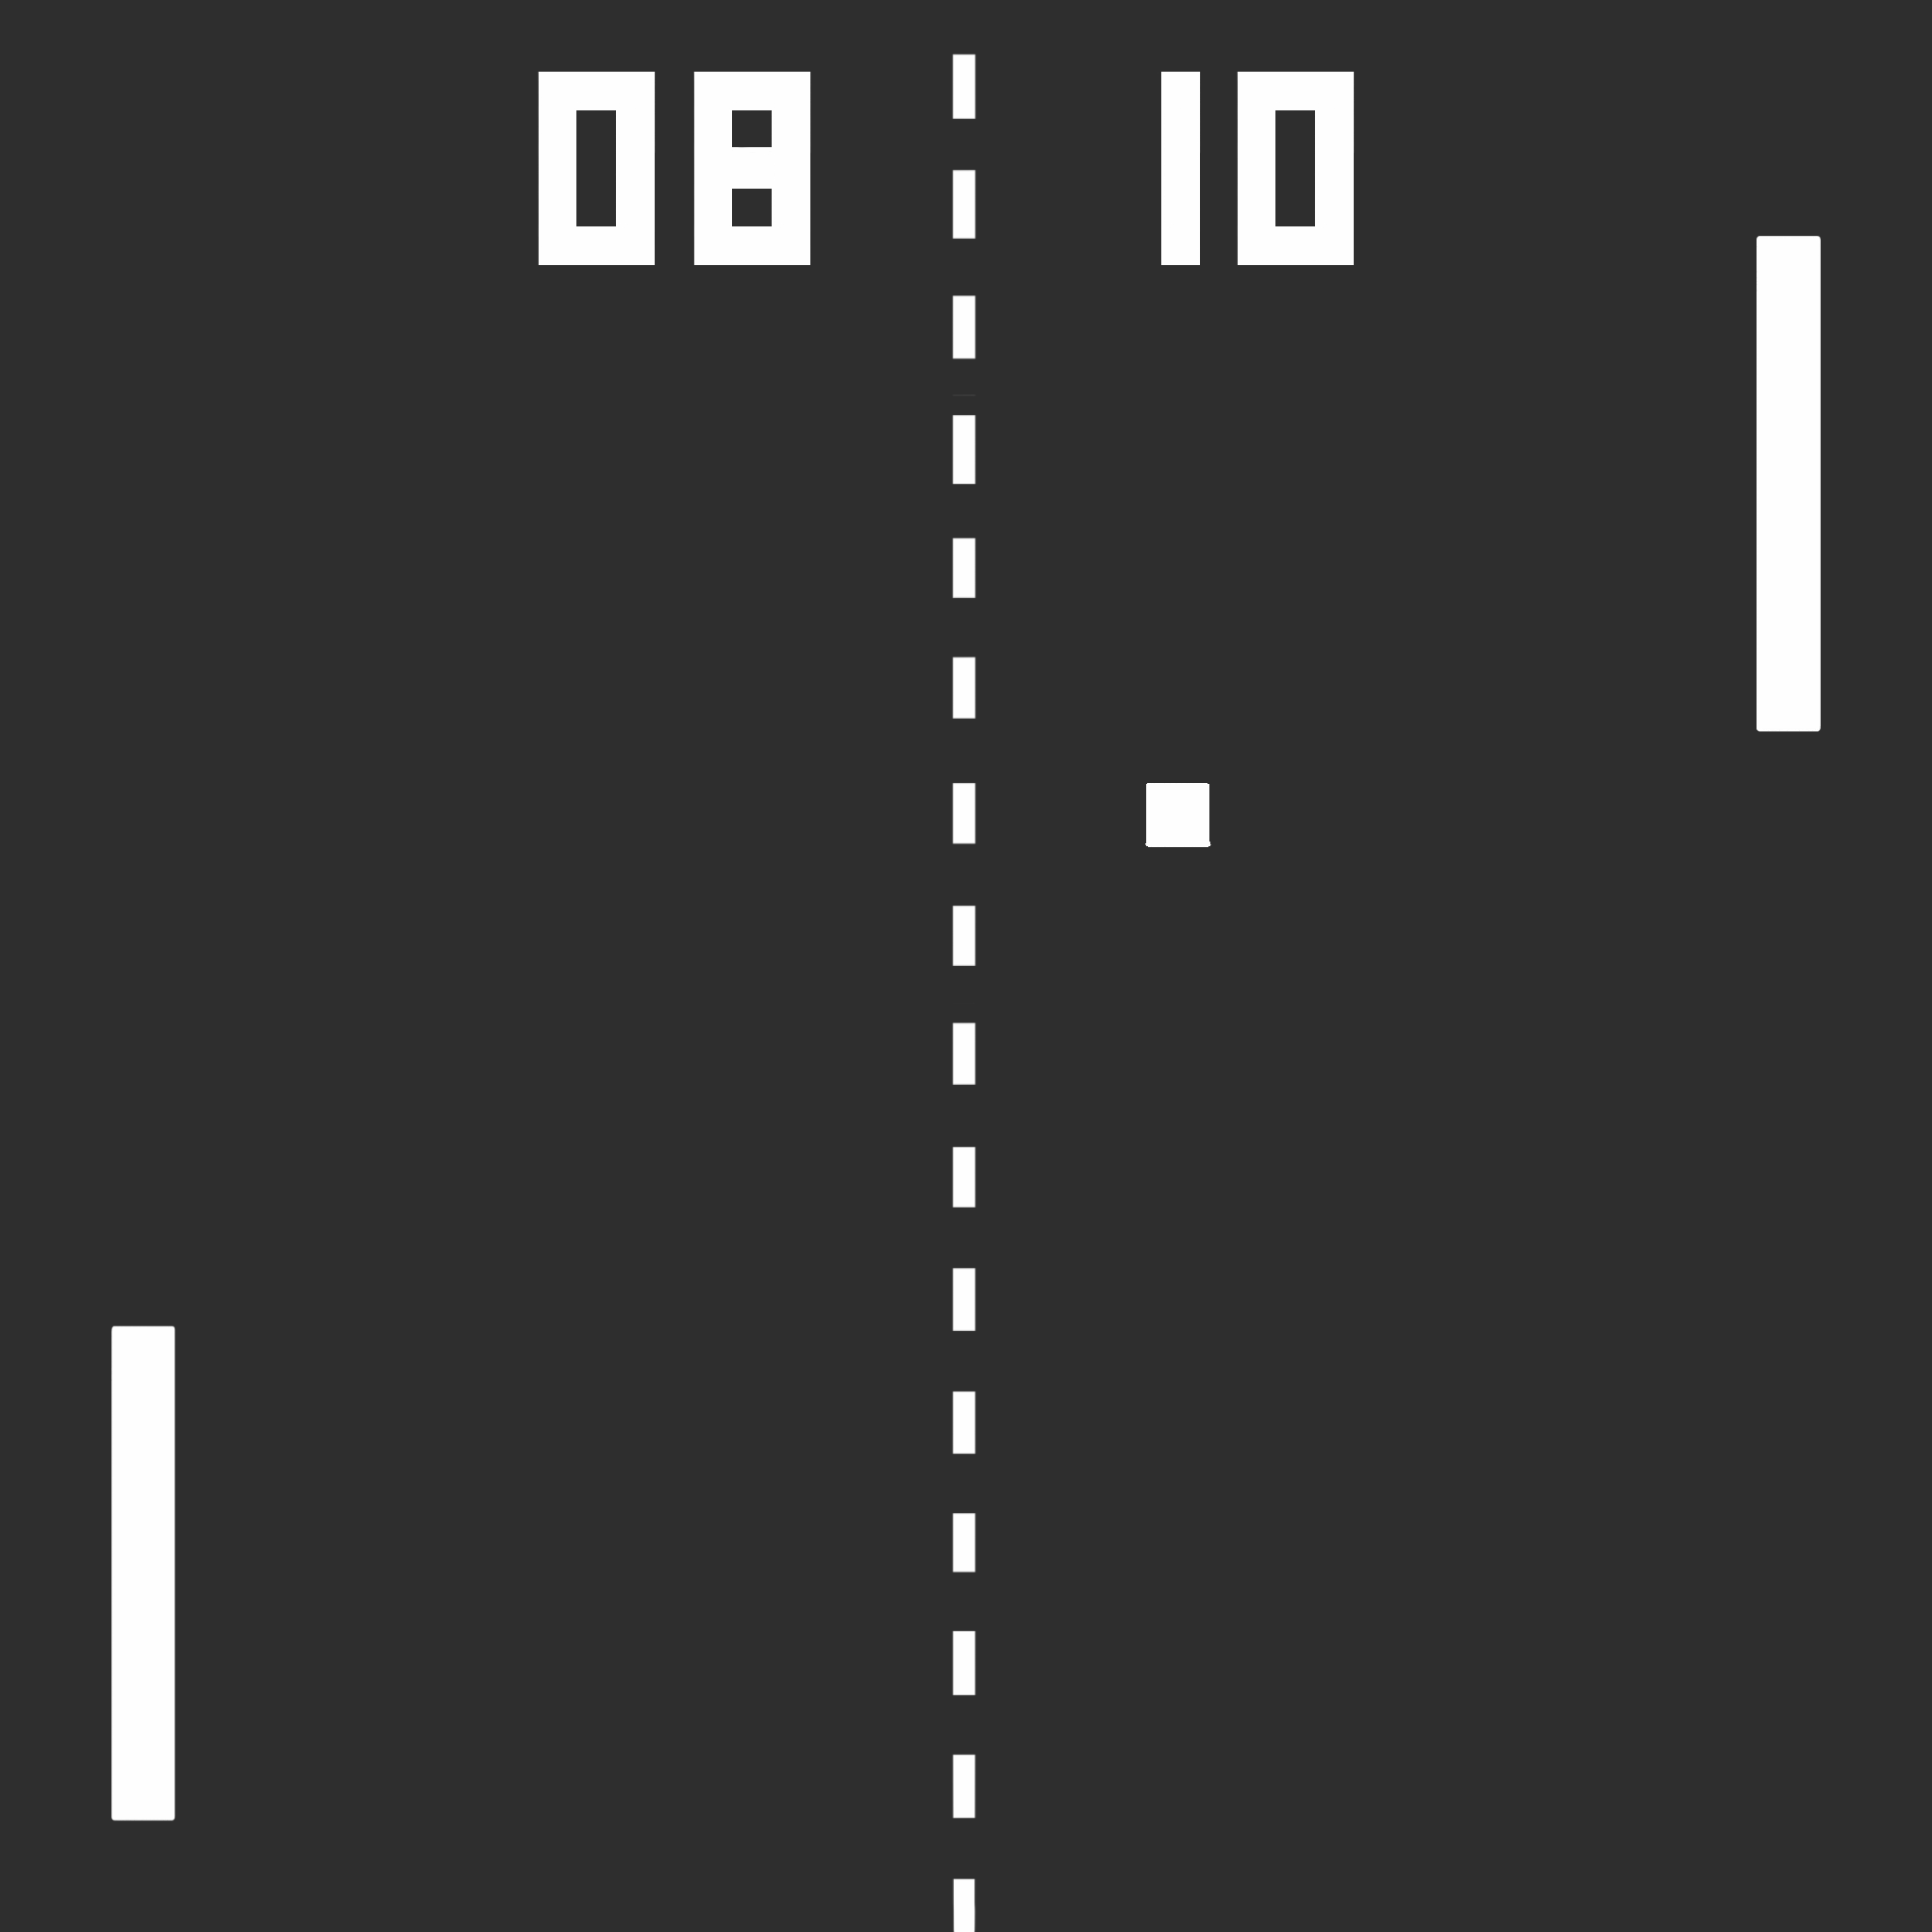
\includegraphics[height=4cm]{/home/cerfe/ATELIER-GROUPPROJECT/sa-project/pub/web/html/gen1_pong/media/IMG2.png}
 
 

The three members built a cabin cruiser capable of holding the game and to test its commercial potential they put it in a local bar, Andy Capp's Cavern in Sunnyvale, which was their favourite. In a few days Pong turned out to be an incredible success. Atari immediately began large-scale production and the game was released on 29th November 1972. At the end of 1974 Atari sold more than 8,000 units and exported all over the world. With Pong, the video game industry was born.

Thanks to Pong, Atari became the market leader in digital entertainment until the 1980s. Between 1974 and 1976, Steve Jobs and Steve Wozniak used disassembled parts from consoles and other Atari devices, and with the fundamental help of several engineers from the Bushnell-based company, they were able to build their first personal computer and found their company, Apple. In 1976 Steve Jobs asked Bushnell if he wanted to buy 33 of the company's shares for 50,000. Bushnell refused. Following the 1983 video game crisis, Atari was closed on 1 July 1984 and divided into two separate companies: Atari Corporation and Atari Games.
 
 
 \includegraphics[height=4cm]{/home/cerfe/ATELIER-GROUPPROJECT/sa-project/pub/web/html/gen1_pong/media/IMG3.jpg}
 
 
 
 
 \subsection{Features }
 When Pong was designed, the graphics were not based on matrices or pixels. Scanning lines (lines into which an image is divided: a strip of pixels) were used for programming. All the contacts (ball-stick and ball-border) were handled by the gates (and, or, ...). Several features contributed to the success of PONG:
 
 
 It's the first arcade video game called "coin-op", that is, it runs on coins (usually a quarter). 
 For the first time a video game is accessible to everyone at a low cost. The playability was simple.   
 It was possible to give effects to the shot by hitting the ball at the last moment, which gave more chances to score point. 
 
 \subsection{sources }
 
 \href{https://www.britannica.com/topic/electronic-sports-game}{https://www.britannica.com/topic/electronic-sports-game }
 \href{http://www.pongmuseum.com/}{http://www.pongmuseum.com/ }
 \href{https://www.landesmuseum.ch/landesmuseum/ausstellungen/wechselausstellungen/2020/games/medien/la-storia-dei-videogiochi-it.pdf}{https://www.landesmuseum.ch/landesmuseum/ausstellungen/wechselausstellungen/2020/games/medien/la-storia-dei-videogiochi-it.pdf }
 \href{https://www.georgefiorini.eu/hub-videogames.php}{https://www.georgefiorini.eu/hub-videogames.php }
 
 \newpage\pageHeader{Pong Home}{1974-08-03}{Samuel Corecco}{A page about the console Pong Home}
 \subsection{Home Pong }
     
 \includegraphics[height=4cm]{/home/cerfe/ATELIER-GROUPPROJECT/sa-project/pub/web/html/gen1_pong_Home/media/IMG1.png}
 
 
 \subsection{History }
 After the success of Pong, Atari decided to develop new products. So it was that in 1974, Harold Lee, Atari's engineer, proposed to produce a homemade version of "PONG". Lee worked with Alan Alcorn on the first projects, basing them on the digital technology used in their games. Lee worked on logic and design and Alcorn worked on debugging in the evenings. Later the team was joined by engineer Bob Brown who assisted them in the construction of the prototype. The prototype was a device attached to a pedestal full of wires, which was eventually replaced by a chip created in 1974 by Alcorn and Lee.
           
 
 \includegraphics[height=4cm]{/home/cerfe/ATELIER-GROUPPROJECT/sa-project/pub/web/html/gen1_pong_Home/media/IMG2.jpg}
 
 
          On August 3, 1975, Atari launched Home Pong, which consisted of a small console that could be connected to the TV and two knob controllers included in the console's shell. Atari presented its console to several toy retailers and electronics shops,
         
 \includegraphics[height=4cm]{/home/cerfe/ATELIER-GROUPPROJECT/sa-project/pub/web/html/gen1_pong_Home/media/IMG4.png}
 
           but no one was interested in the product because it was considered too expensive and of little interest. The asking price was about 100 (equivalent to over 400 nowadays). Atari set up a Home Pong stand at the American Toy Fair (a trade show) in New York again without success. Fortunately, the company was able to reach an agreement with Sears. For the Christmas period 1975, Sars 150'000 units and to satisfy this order Atari bought a new factory. The model was manufactured under the name "Tele-Games" by Sears. The console proved to be a great success: during the Christmas period of 1975 as many as 150,000 units were sold in the United States and it was the most commercialised item in the Sears catalogue that had requested exclusivity for the sale. In 1976 Atari released a version with its own brand.
           
 
 \includegraphics[height=4cm]{/home/cerfe/ATELIER-GROUPPROJECT/sa-project/pub/web/html/gen1_pong_Home/media/IMG3.jpg}
 
 
 \subsection{Features }
 The console had one important feature: Alcorn and Lee made a single chip that calculated the score and provided an attractive sound. It was the highest performing chip used in a consumer product.
 
 
 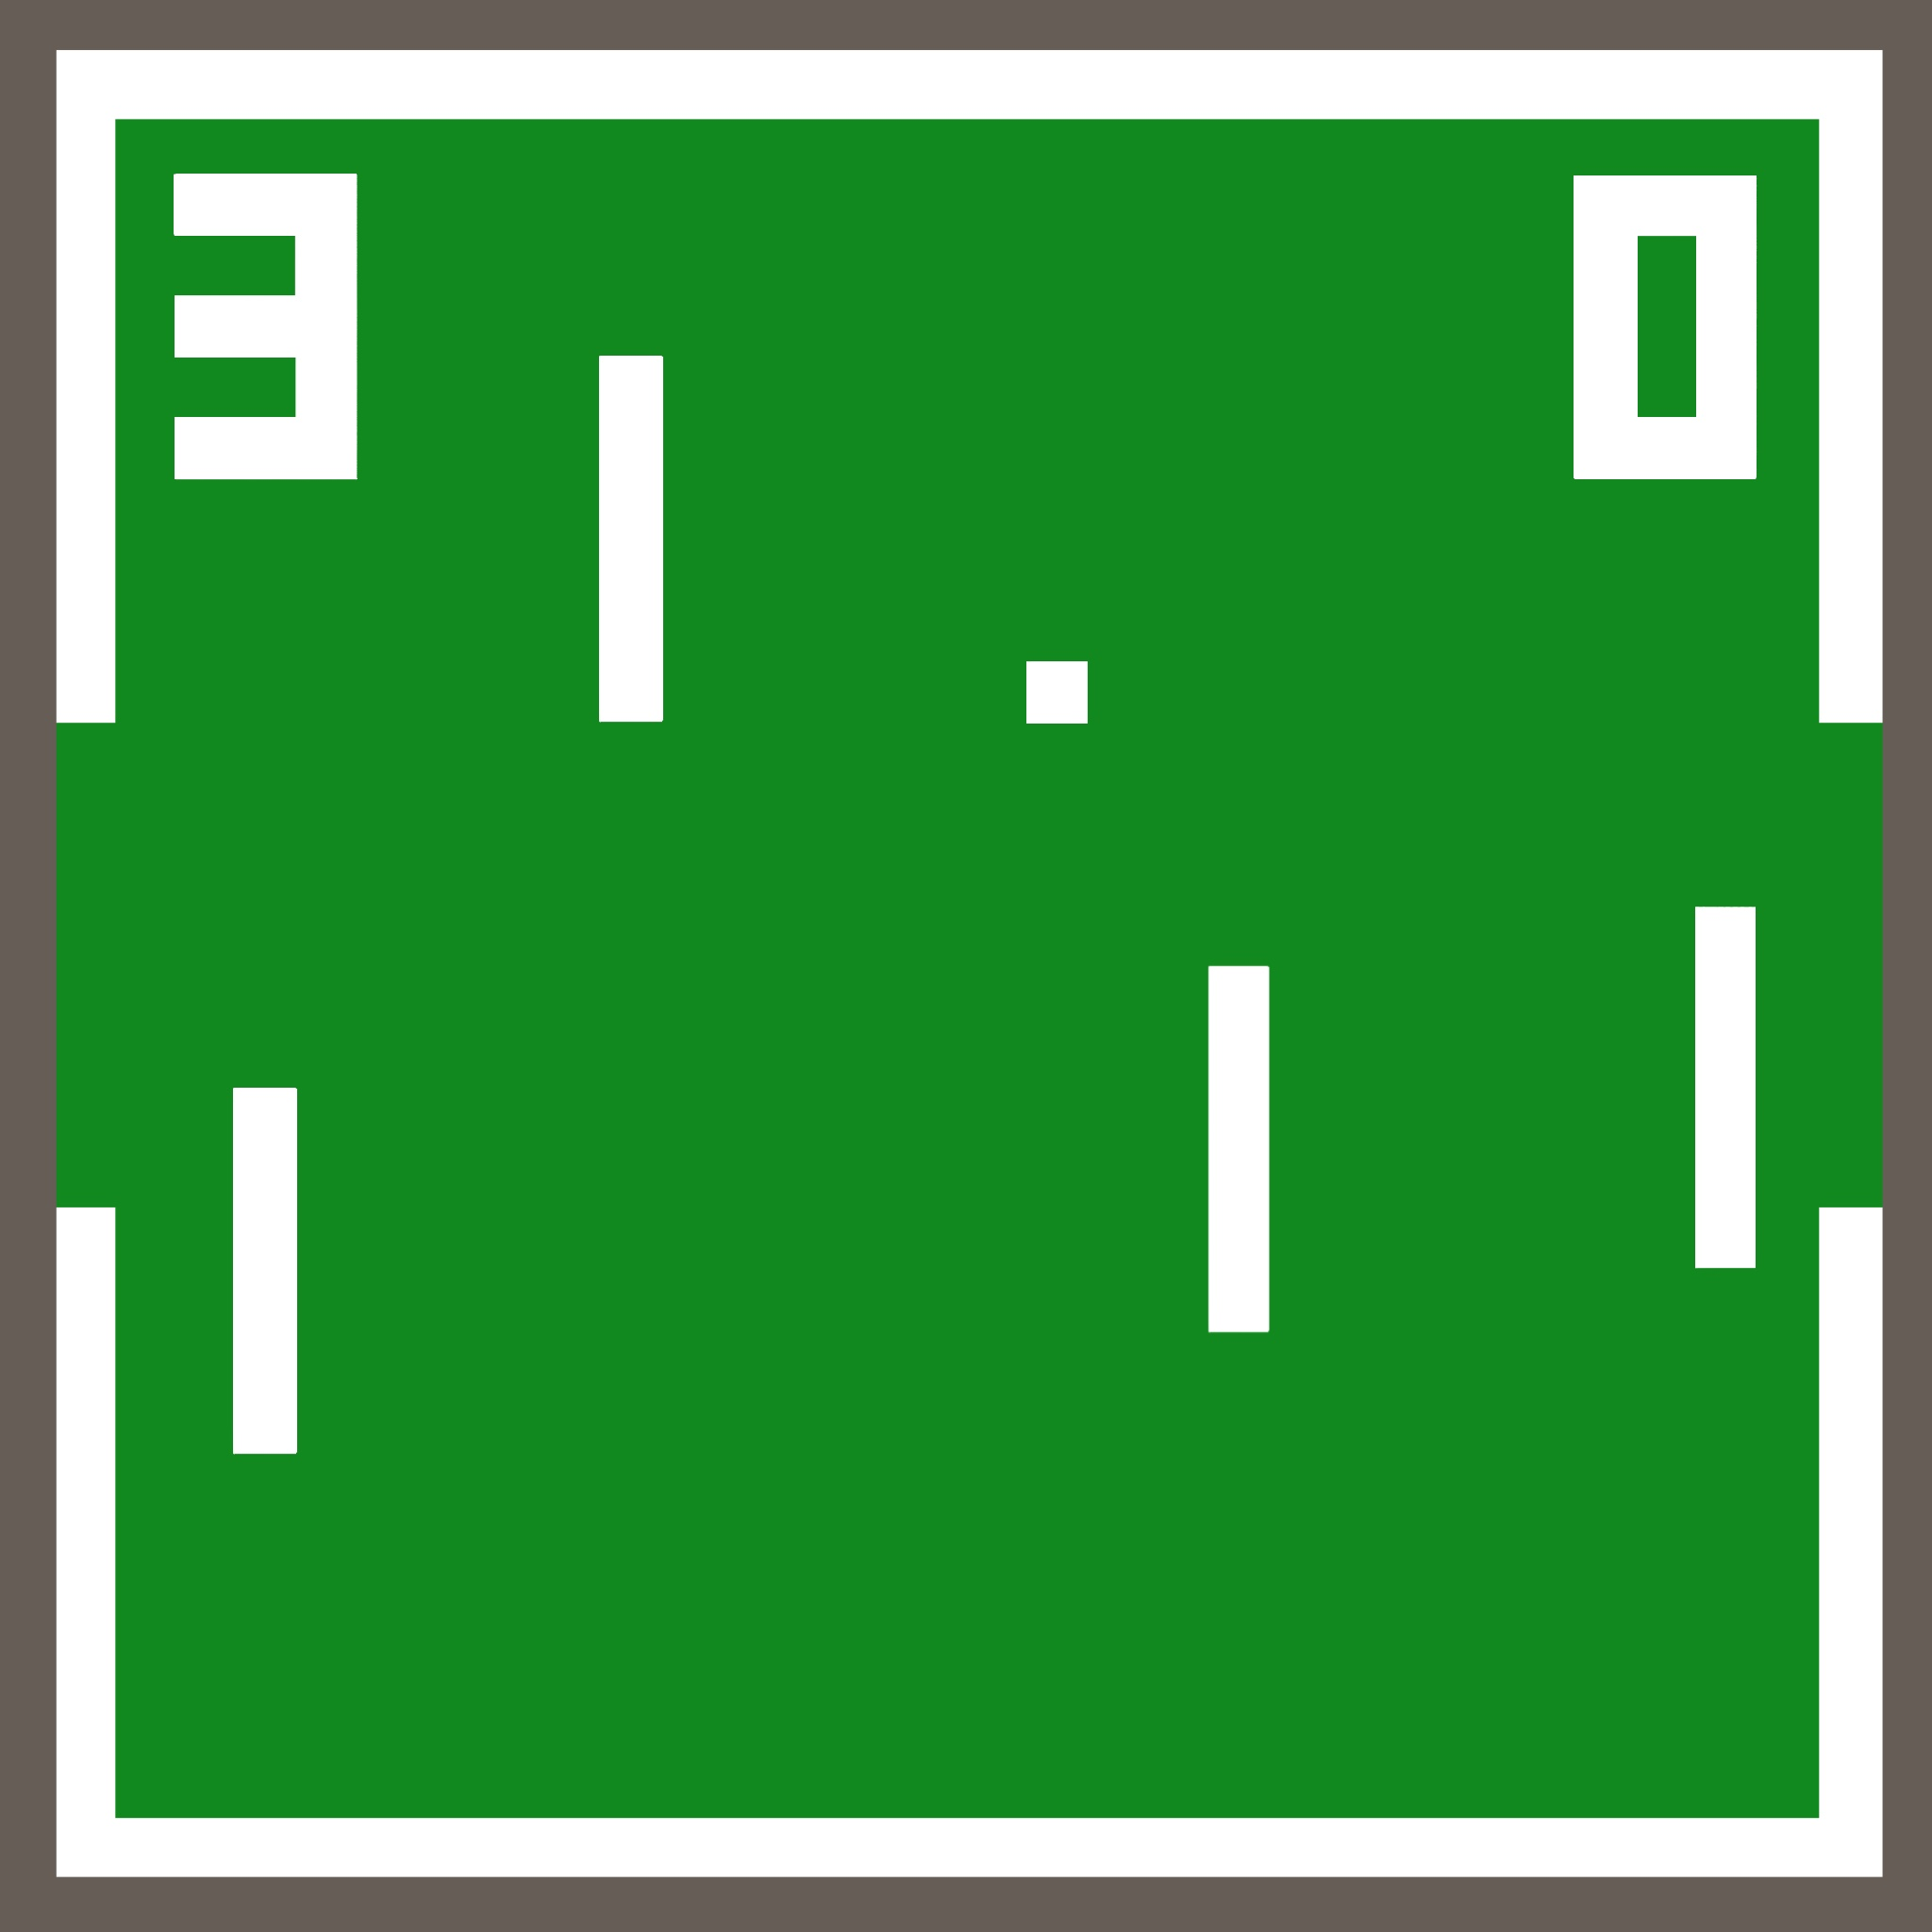
\includegraphics[height=4cm]{/home/cerfe/ATELIER-GROUPPROJECT/sa-project/pub/web/html/gen1_pong_Home/media/IMG5.jpg}
 
          The image was obtained by interpolating the scanning lines of the electronic signal coming from the cathode ray tube of the TV. The contacts between the ball and racket and between the ball and the edges of the field were made with logical components.The game was in black and white like most televisions at that time.
          In 1978 the American General Instruments managed to produce at low cost and in large quantities microchips specifically dedicated to this game, the most famous of which was the AY-3-8500 model able to offer 6 different games and more setting options. This allowed many companies to enter the video game market which created a huge amount of Atari "Home Pong" clones. This increased the mass production of the video game and its popularity at home. The large number of "PONG" clone consoles started a real video game market. The console was the videgame itself, so in this generation there were more versions of the same, one for each type of game.
           
 
 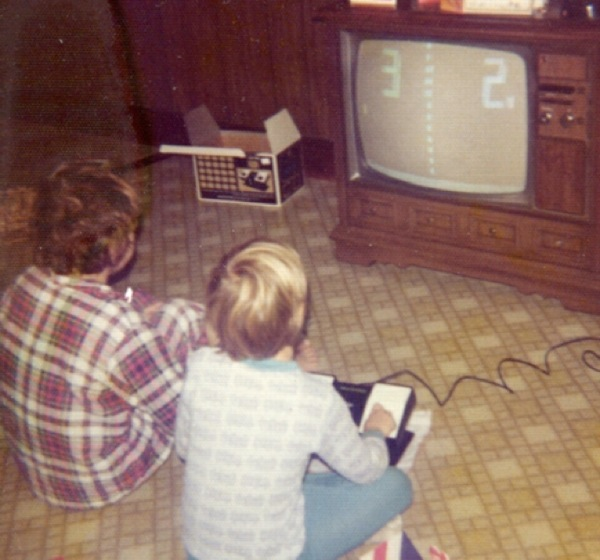
\includegraphics[height=4cm]{/home/cerfe/ATELIER-GROUPPROJECT/sa-project/pub/web/html/gen1_pong_Home/media/IMG6.jpg}
 
 
 \subsection{sources }
 
 \href{http://www.atarimuseum.com/videogames/dedicated/homepong.html}{http://www.atarimuseum.com/videogames/dedicated/homepong.html }
 \href{https://spectrum.ieee.org/view-from-the-valley/tech-history/cyberspace/atari-alumni-talk-about-the-tall-tales-the-told}{https://spectrum.ieee.org/view-from-the-valley/tech-history/cyberspace/atari-alumni-talk-about-the-tall-tales-the-told }
 \href{https://www.metv.com/stories/the-atari-home-pong-console-is-40-years-old}{https://www.metv.com/stories/the-atari-home-pong-console-is-40-years-old }
 \href{https://breakingtech.it/atari-pong-la-storia-dei-videogiochi/}{https://breakingtech.it/atari-pong-la-storia-dei-videogiochi/ }
 \href{http://www.pong-story.com/atpong2.htm}{http://www.pong-story.com/atpong2.htm }
 \href{https://www.wikiwand.com/it/Storia_dei_videogiochi#/1972:_la_nascita_della_Atari}{https://www.wikiwand.com/it/Storiadeivideogiochi/1972:lanascitadellaAtari }
 \href{https://en.wikipedia.org/wiki/Pong}{https://en.wikipedia.org/wiki/Pong }
 \href{https://en.wikipedia.org/wiki/AY-3-8500}{https://en.wikipedia.org/wiki/AY-3-8500 }
 \href{https://en.wikipedia.org/wiki/Ted_Dabney}{https://en.wikipedia.org/wiki/TedDabney }
 \href{https://en.wikipedia.org/wiki/Atari}{https://en.wikipedia.org/wiki/Atari }
 
 \newpage\pageHeader{TV Tennis Electrotennis}{1975-12-12}{Enrico Benedettini}{The first japanese home console ever.}
 \subsection{History }
 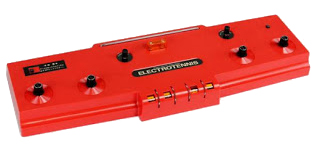
\includegraphics[height=4cm]{/home/cerfe/ATELIER-GROUPPROJECT/sa-project/pub/web/html/gen1_tv_tennis_electrotennis/media/TV_Tennis_Electrotennis.jpg}
 
          The  \textbf{Tv Tennis Electrotennis }  is a home dedicate console appertaining to the first generation.
          It was released by  \textbf{Epoch Co. }  together with  \textbf{Magnavox }  on  September 12 th 
 \textbf{1975 } , several months before the  \textbf{Home Pong }  in America, only in Japan becoming
          the  \textbf{first video game console ever launched }  in Japan.  
          Its cost was 19 000 yen and sold about 10 000 units.
         
 
 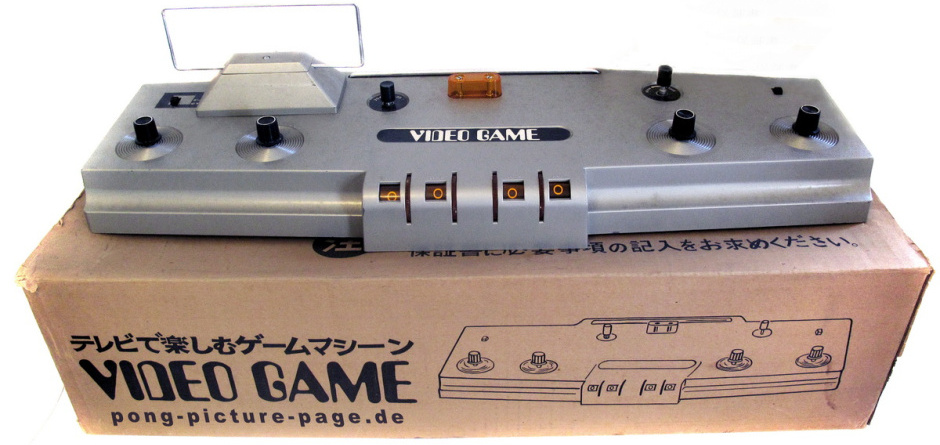
\includegraphics[height=4cm]{/home/cerfe/ATELIER-GROUPPROJECT/sa-project/pub/web/html/gen1_tv_tennis_electrotennis/media/electrotennis-silver.jpg}
 \subsection{Console }
 
          This console implemented the Pong game but added a unique feature: which was the  \textbf{UHF antenna } , that allowed it to connect wirelessly to the TV.
          There also exists a model not famous at all with a silver-grey cover, as shown in the figure.
         
 
 
 
 
 
 References 
 
 \href{https://it.wikipedia.org/wiki/TV_Tennis_Electrotennis}{TV Tennis Content and Pic }
 
 @ Enrico Benedettini 
 
 
 \newpage\pageHeader{coleco teslar}{1976-01-01}{Samuel Corecco}{A page about the coleco Teslar series}
 \subsection{Coleco Telstar sieries }
     
 \includegraphics[height=4cm]{/home/cerfe/ATELIER-GROUPPROJECT/sa-project/pub/web/html/gen1_teslar/media/IMG1.png}
 
 
 \subsection{History }
 Coleco was the first company to use General Instrument's AY-3-8500 chip in a home video game in 1976 with the Coleco Telstar console. Coleco Telstar is a Home Pong clone. Thanks to its low price (50), it was able to sell over a million units in a single year. The large number of consoles produced led to a shortage in the market of chips produced by General Instrument, which mainly affected the competition.  In total, Coleco produced 14 Coleco Telstar series consoles.
           
 
 \includegraphics[height=4cm]{/home/cerfe/ATELIER-GROUPPROJECT/sa-project/pub/web/html/gen1_teslar/media/IMG2.jpg}
 
 
 \subsection{Features }
 The first edition of Coleco Telstar had two integrated controllers.
          A three-position switch allowed to control the difficulty (beginner, advanced and expert. The Coleco models were sold partially assembled: buyers had to mount the knobs and stickers on the console, a choice that seems to have been wanted to reduce costs. The first console was simple and offered three games: tennis, hockey and handball). The Telstar was a basic model that only partially exploited the possibilities of the AY-3-8500 chip. This model was followed by others with more advanced features. In total, Coleco produced 14 Coleco Telstar series consoles until 1978. These included the Telstar Colormatic (1977, similar but in colour), the Regent (in black and white with three additional games), the Colortron, the Telstar Sportsman and Telstar Combat (1977) and finally the Arcade (1978) with interchangeable cartridges. The wide range of products and the crisis of interest in the Pong game led Coleco to bankruptcy in 1980.
 
 
 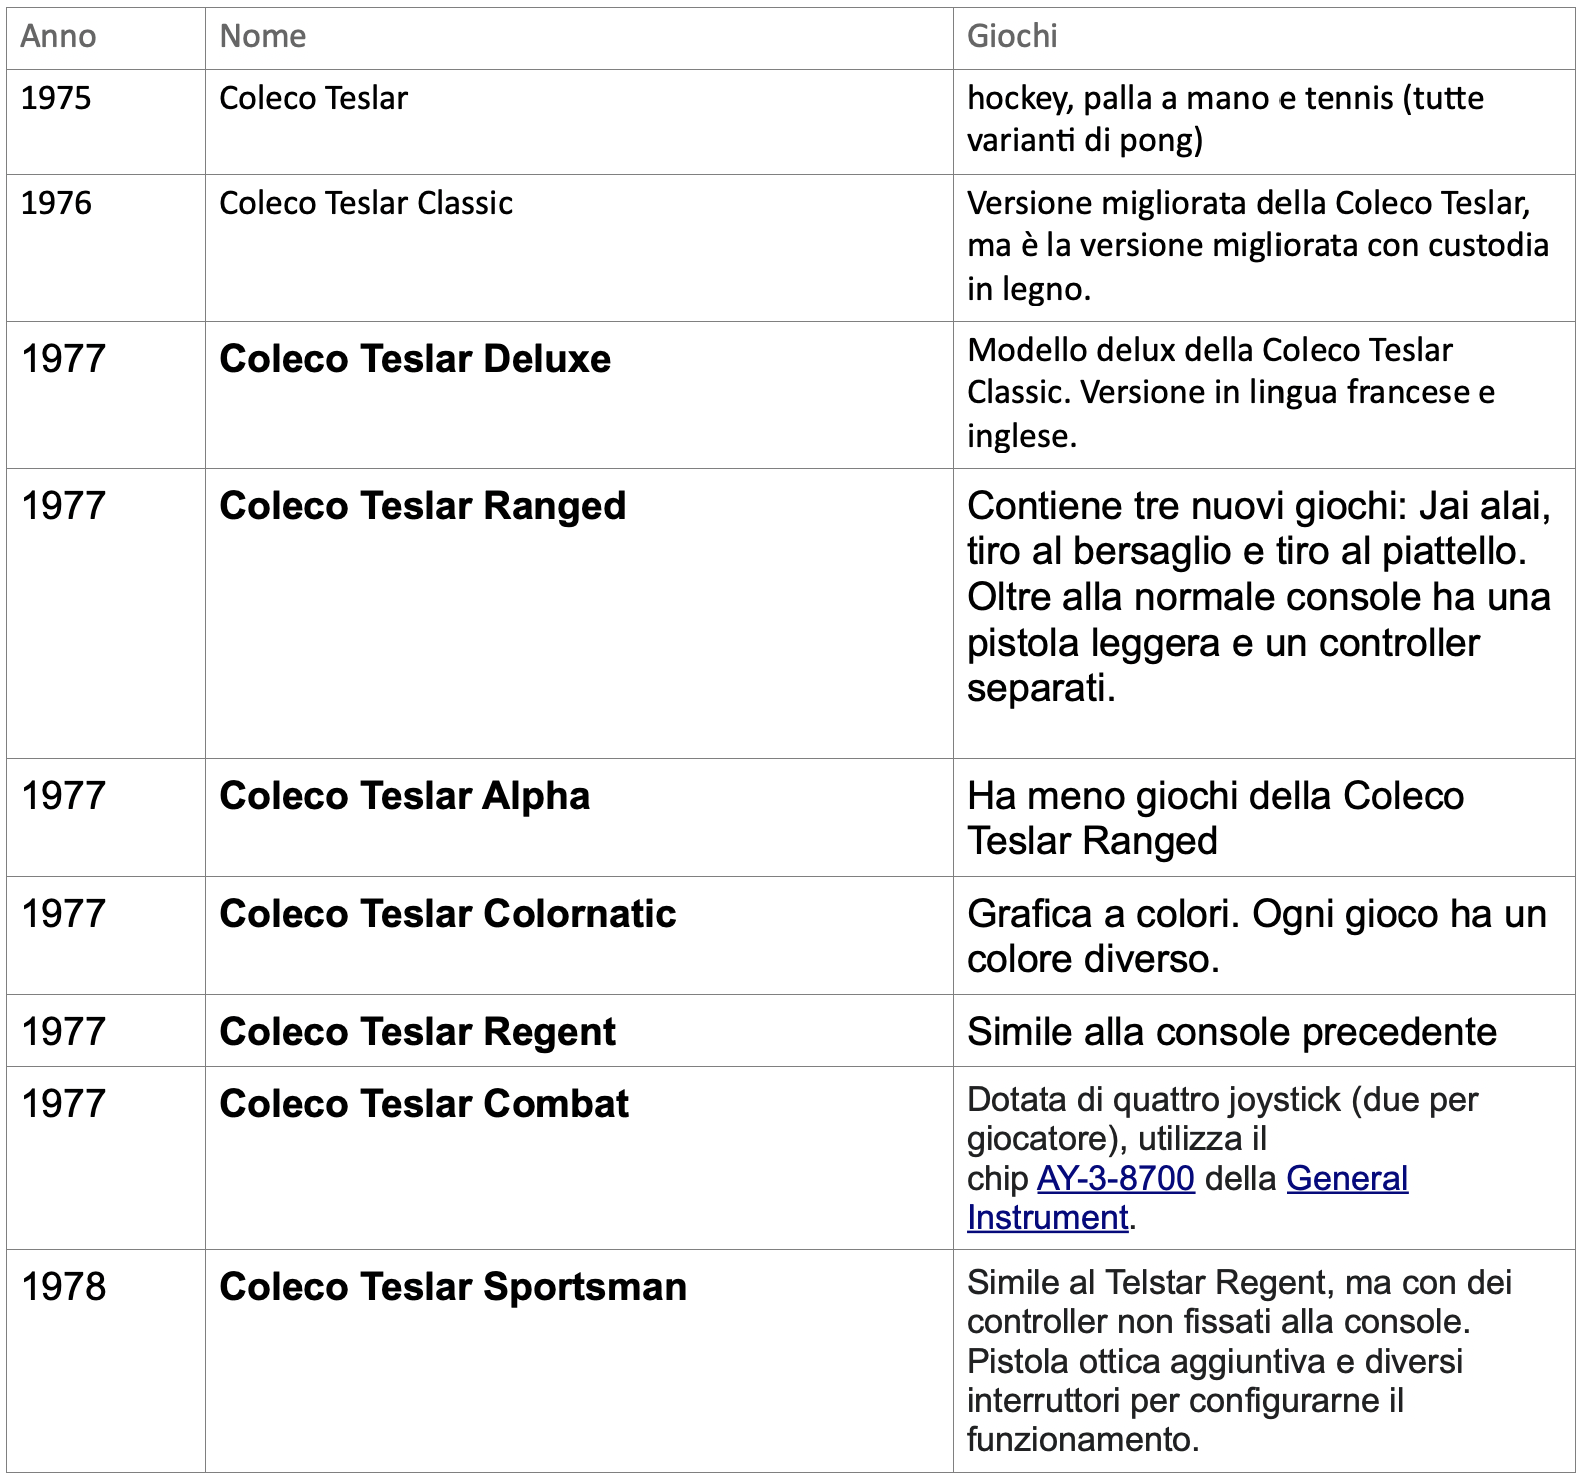
\includegraphics[height=4cm]{/home/cerfe/ATELIER-GROUPPROJECT/sa-project/pub/web/html/gen1_teslar/media/IMG3.png}
 
      These models stood out for their shapes.The Arcade version proved to be a revolution for the times. It consisted of three types of controllers: one side held the knobs, another had a mini steering wheel and gear lever, and a third had a plastic shotgun aimed at the screen. Of vital importance, it was also shaped like a triangle.

       
 \includegraphics[height=4cm]{/home/cerfe/ATELIER-GROUPPROJECT/sa-project/pub/web/html/gen1_teslar/media/IMG4.png}
 
 
 \subsection{sources }
 
 \href{https://www.go42.net/retro-gaming/la-console-colecovision/}{https://www.go42.net/retro-gaming/la-console-colecovision/ }
 \href{http://www.dizionariovideogiochi.it/doku.php?id=coleco_telstar}{http://www.dizionariovideogiochi.it/doku.php?id=colecotelstar }
 \href{https://en.wikipedia.org/wiki/Coleco}{https://en.wikipedia.org/wiki/Coleco }
 
 \newpage\pageHeader{Handheld Systems}{1976-01-01}{Enrico Benedettini}{The first handheld consoles ever.}
 \subsection{Introduction }
 
          The Handheld systems were only dedicated consoles until the arrival, with the second generation, of
          the  \textbf{Microvision }  that provided the possibility to insert different games. Also, since the advent of
          the fourth generation  \textbf{Game Boy } , all the others handled systems were eclipsed.  
 
 
 \subsection{Consoles }
 
          Between  \textbf{1977 }  and  \textbf{1982 } , the first handheld systems came out, passing from the first
           \textbf{Mattel Auto Race }  until the very first handheld system from Microvision.
         
 
 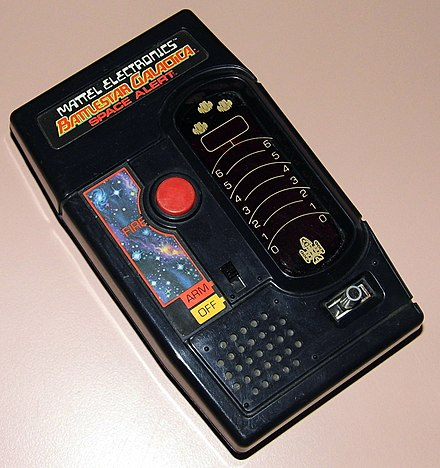
\includegraphics[height=4cm]{/home/cerfe/ATELIER-GROUPPROJECT/sa-project/pub/web/html/gen1_handheld_systems/media/Battlestar_Galactica.jpg}
 \subsubsection{Mattel Auto Race }
 
 \textbf{Mattel Electronics Auto Race }  was the  \textbf{first handheld game ever }  to be totally digital.
            It was released in  \textbf{1976 } , pioneering this category of games. The games were based on avoiding other cars
            arriving from the top while the player has to reach the top 4 times (4 laps) before the time ends (99 seconds,
            which is the limit in only two digits). It was also possible to change the velocity in a range of 4, but by doing
            this, the other cars will be as fast as we set, too.  
            Mattel also produced a very similar version of this product, the  \textbf{Battlestar Galactica } .
            Here the player rests at the bottom while trying to shoot the space navies and if manages, he gains points.
           
 
 
 
 \subsubsection{Mattel Football }
 \includegraphics[height=4cm]{/home/cerfe/ATELIER-GROUPPROJECT/sa-project/pub/web/html/gen1_handheld_systems/media/Mattel-Football.jpg}
 
 \textbf{Football }  was launched in  \textbf{1977 }  and foresaw to make possible a football game on a
            9-yards camp. According to a preview that was then discovered to be bad due to the high demand, the market trend was thought to be bad.
              The market trend was thought to be bad, according to a preview that was then discovered to be
            bad due to the high demand.  It sold more than 500 000 units!
           
 
 
 
 \includegraphics[height=4cm]{/home/cerfe/ATELIER-GROUPPROJECT/sa-project/pub/web/html/gen1_handheld_systems/media/Simon.jpg}
 \subsubsection{Simon }
 
 \textbf{Simon }  was a  \textbf{memory skill }  game where the player was supposed to repeat the sequence
            said by the console pressing the buttons, which lighted on while sounding that tone.
           
 
 
 
 \subsubsection{Electronic Quarterback }
 \includegraphics[height=4cm]{/home/cerfe/ATELIER-GROUPPROJECT/sa-project/pub/web/html/gen1_handheld_systems/media/Coleco_Electronic_Quarterback.jpg}
 
 \textbf{Electronic Quarterback }  was out in  \textbf{1978 }  and differs from the other handheld systems
            giving the possibility for the quarterback, adding two blockers, to pass the ball. But the game is still
            really similar to Football, but focused on the quarterback passing and running.
           
 
 
 
 
 References 
 
 \href{https://en.wikipedia.org/wiki/Simon_(game)}{Simon }
 \href{https://en.wikipedia.org/wiki/Mattel_Auto_Race}{Mattel Auto Race }
 \href{https://en.wikipedia.org/wiki/Electronic_Quarterback}{Electronic Quarterback }
 \href{https://www.handheldmuseum.com/Mattel/FB.htm}{Football Image and Mattel Content }
 \href{https://en.wikipedia.org/wiki/First_generation_of_video_game_consoles#Handheld_systems}{Content Source }
 
 @ Enrico Benedettini 
 
 
 \newpage\pageHeader{Nintendo Color TV-Gameseries}{1977-06-01}{Samuel Corecco}{A page about the Nintendo Color TV-Gameseries}
 \subsection{Nintendo Color TV-Gameseries }
     
 \includegraphics[height=4cm]{/home/cerfe/ATELIER-GROUPPROJECT/sa-project/pub/web/html/gen1_tv_game nintendo/media/IMG1.png}
 
 
 \subsection{History }
 
 
 \includegraphics[height=4cm]{/home/cerfe/ATELIER-GROUPPROJECT/sa-project/pub/web/html/gen1_tv_game nintendo/media/IMG5.jpg}
 
          Nintendo Corporation, Ltd (Japanese for "Nintendo" () means "fortune that comes from the sky") is a Japanese game and console developer based in Kyto, Japan.
Before it was involved in video games, Nintendo produced playing cards and toys. In 1970 it abandoned everything to enter the rapidly growing video game market. In 1975 it developed the Othello Computer, with which Othello was played. Shortly afterwards other games such as Sheriff and Space Fever were released. At first it was not very successful.
In 1977, with the help of Mitsubishi Electric Nintendo created the Color TV-Game, a series of five consoles containing variations of Pong. He introduced a very important and innovative element: colour.  
 
 \subsubsection{Color TV-Game 6 }
 The first Color TV-Game model contained six variants of PONG, called "Light Tennis" and was cheaper than its competitors ( 9,800). The console was powered by batteries or power supplies sold separately. After the console was released, an improved version came out, with a white outer casing and power supply removed.
Later versions were called Color TV Game 15, Color TV Racing 112, Color TV Block Kusure and Computer TV Game. In all, the series sold three million units, making it the world's best-selling first-generation console series. In 1980, 70 of Japanese gamers owned a Nintendo system.
 
 \includegraphics[height=4cm]{/home/cerfe/ATELIER-GROUPPROJECT/sa-project/pub/web/html/gen1_tv_game nintendo/media/IMG2.jpg}
 
 
 \subsubsection{Color TV-Game 15 }
 
  On 8 June 1977, Nintendo released the Color TV-Game 15, sold for 15,000. The console had controllers that could be detached.
 
 \includegraphics[height=4cm]{/home/cerfe/ATELIER-GROUPPROJECT/sa-project/pub/web/html/gen1_tv_game nintendo/media/IMG3.jpg}
 
 
 \subsubsection{Color TV Game Racing 112 }
 
  On 8 June 1978 the Color TV Game Racing 112 was released. The console was larger than its predecessors and its price was 18,000, later lowered to 12,000. It was eventually reduced to 5,000. It contains a racing game. The console is also equipped with two controllers, so you can play multiplayer games.
 
 \includegraphics[height=4cm]{/home/cerfe/ATELIER-GROUPPROJECT/sa-project/pub/web/html/gen1_tv_game nintendo/media/IMG4.png}
 
 
 \subsubsection{Color TV Game Block Kuzush }
 
 
 \includegraphics[height=4cm]{/home/cerfe/ATELIER-GROUPPROJECT/sa-project/pub/web/html/gen1_tv_game nintendo/media/IMG8.png}
 
 On 23 April 1979 the console was released at a price of  13,500. This console is the first 100 Nintendo console. It i salso the first Nintendo video game with the Nintendo name prominently displayed on the console. The console includes six variations of Breakout, an arcade game released in America by Atari. The Nintendo clone is called Block Fever.
 
 
 \includegraphics[height=4cm]{/home/cerfe/ATELIER-GROUPPROJECT/sa-project/pub/web/html/gen1_tv_game nintendo/media/IMG6.png}
 
 
 \subsubsection{Computer TV Game }
 
  Released in 1980, it is the last console in the series. The popularity of these consoles was declining and the Computer TV Game was produced in limited quantities. The console contains an advanced CPU, which allows the player to challenge the computer. This addition greatly increased the price of the console.
 
 
 \includegraphics[height=4cm]{/home/cerfe/ATELIER-GROUPPROJECT/sa-project/pub/web/html/gen1_tv_game nintendo/media/IMG7.png}
 
 
 \subsection{sources }
 
 \href{https://en.wikipedia.org/wiki/Color_TV-Game}{https://en.wikipedia.org/wiki/ColorTV-Game }
 \href{https://it.wikipedia.org/wiki/Color_TV_Game}{https://it.wikipedia.org/wiki/ColorTVGame }
 \href{http://www.computinghistory.org.uk/det/20732/Color-TV-Game-6/}{http://www.computinghistory.org.uk/det/20732/Color-TV-Game-6/ }
 \href{https://nintendo.fandom.com/wiki/Color_TV-Game_6}{https://nintendo.fandom.com/wiki/ColorTV-Game6 }
 \href{https://nintendo.fandom.com/wiki/Color_TV-Game_15}{https://nintendo.fandom.com/wiki/ColorTV-Game15 }
 \href{https://nintendo.fandom.com/wiki/Color_TV_Racing_112}{https://nintendo.fandom.com/wiki/ColorTVRacing112 }
 \href{https://nintendo.fandom.com/wiki/Computer_TV_Game}{https://nintendo.fandom.com/wiki/ComputerTVGame }
 
 \newpage\chapter{gen2}\newpage\pageHeader{FAIRCHILD CHANNEL F}{1976-08-08}{ALESSANDRO CRAVIOGLIO}{The Fairchild channel F, a direct competitorof the Atari2600}
 \subsection{The Console }
 \subsubsection{A bit of History }
 \begin{longtable}{p{1mm}|l|l|}\hline
 
 & 
          The Fairchild Channel F was the first programmable console based on ROM cartridges and started the second generation of consoles.
          It was put on sale by Fairchild Semiconductor ( a division of the parent company) in August 1976 at a cost of 169.95 US dollars.
          Initially called Video Entertainment System or VES, it took the name Channel F in 1977 after Atari presented its VCS console.
         
 & \includegraphics[height=4cm]{/home/cerfe/ATELIER-GROUPPROJECT/sa-project/pub/web/html/gen2_fairchild_channel_f/media/fairchild_true_console.jpeg}
 \\\hline
 \end{longtable}
 \subsubsection{The Hardware }
 
          The Channel F electronics was designed using the Fairchild F8 microprocessor as CPU.
          The F8 CPU was very complex and offered many more input and output lines than other chips.
          The CPU was powerful enough to write games with artificial intelligence to allow you to play
          "against the computer", when other consoles only allowed you to play against another human player.
          The graphics of the console was rudimentary: the screen had a resolution of 12864 pixels;
          for the background it could display only 1 color chosen among 4 for each line of the image, while for the
          main graphics you could choose only between 3 main colors, red, green and blue, or white in case the background was black.
          The RAM memory was 64 bytes.
           
 CPU: Fairchild F8 (8-bit) 
 RAM: 2KB, plus 64 bytes of scratchpad memory 
 Input: two controllers 
 Output: wired video signal 
 
 
 \subsection{Games Supported }
 \begin{longtable}{p{1mm}|l|l|l|}\hline
 
 & \includegraphics[height=4cm]{/home/cerfe/ATELIER-GROUPPROJECT/sa-project/pub/web/html/gen2_fairchild_channel_f/media/game_cartridges.jpeg}
 
 & 
 & The amonunt of games released with this console is not huge: only twenty-seven games cartridges were released
          for the Fairchild Channel F. It has be to be said that several of these cartridges were capable of playing
          more games (example: Videocart 1 has Tic-Tac-Toe, Shooting Gallery, Doodle and Quadra Doodle)
          In addition to these, two standard games were sold together with the console: Tennis and Hockey. An unusual
          feature of this console are the incredibly colorful artwork of the games cartridges. Fun fact: the Pac-Man cartridge,
              aka Game Cartridge 27, was released for the Channel F in year 2009.
           
 \\\hline
 \end{longtable}
 \subsection{Impact on the Market and Reception }
 
          The Channel F was launched in November 1976, nearly a year before Ataris VCS console.
           It's renown to be the first console with  \textbf{REMOVABLE GAME CARRTRIDGES } , we could call it the first console with "removable software".
           Its Fairchild F8 microprocessor, low resolution color graphics, and 2K RAM were outclassed by its rival despite its
           far superior joysticks, and its lack of the Ataris much larger software catalog saw it steadily lose ground into the
           1980s despite a hardware revamp. Surprisingly it continued production until 1983,with 250'000 units sold, by which time it must have
           appeared an anachronism when compared to the crop of 8-bit microcomputers. 
 
 @Alessandro Cravioglio 
 
 \newpage\pageHeader{Shoot'em up genre}{1976-11-01}{Manuele Jelmini}{A look at the most important genre of the second generation}
 \subsection{The shoot'em up games genre }
 
 \subsubsection{Description }
 
 
 \textbf{"Shoot'em up" }  (often abbreviated as  \textit{"shmup" }) is a subgenre of shooter games (which is a subgenre of action games).
           While there are many different opinions regarding the exact classification of shoot'em up among the critics, there are some characteristics that are common to most games considered part of this genre;
           for example the  \textbf{restricted movement }  of the playable character (unidirectional "on-rail" movement, fixed position with rotation,...),
           the  \textbf{high amount of enemies/obstacles }  coming from one or more sides of the screen (the  \textit{"them" } part of the genre's name), a  \textbf{score system }  quantifying how well the levels are played, ...  
 
 \begin{longtable}{p{1mm}|l|}\hline
 
 & 
 \\\hline
 
 & \textit{Space Invaders } on  \textit{Atari 2600 }
 \\\hline
 \end{longtable}
 
 \subsubsection{Subgenres }
 
 
           The specifics of these characteristics can also be used to further categorize shoot'em up games into various  \textbf{subgenres }  like " \textbf{side-scrolling shooters } " (featuring a horizontally scrolling action and a side-view perspactive),
           " \textbf{fixed shooters } " (with the action limited to a single screen and unidirectional movements), " \textbf{bullet hell } " (games where the screen is often full of the enemies' projectiles), ...  
 
           Despite the arguably confusing categorization, the gameplay of these games is usually pretty straightforward:  \textbf{move your character }  with the right timing to  \textbf{aim your shots }  and to  \textbf{avoid getting hit } .
           Nowadays most shoot'em up games are easily identifiable by simply looking at the similiarity of gameplay (due to design conventions of the genre) with other "shmup" games.
         
 
 \subsection{The shoot'em up genre in the second generation }
 
 \subsubsection{Important games }
 
 
          Many of the design conventions mentioned previously come from the period of  \textbf{high popularity }  of these kind of games during the  \textbf{second generation }  of video games.
          One of the main responsible for this rise in popularity was  \textbf{\textit{Space Invaders }}  (originally released as an arcade game, then appeared on the Atari 2600 and other consoles later on):
          it was one of the very  \textbf{first games of the genre }  and its success  \textbf{influenced and inspired }  many developers in making shoot'em ups.  
 
 
 \begin{longtable}{p{1mm}|l|}\hline
 
 & 
 \\\hline
 
 & \textit{Asteroids }
 \\\hline
 \end{longtable}
 
 
          Like  \textit{Space Invaders }, many important shoot'em ups like  \textit{Asteroids },  \textit{Defender },  \textit{Galaxian } and  \textit{Missile Command } were ported on the Atari 2600.
          Looking at the  \textbf{best selling games }  on the Atari 2600 we can find many others shoot'em ups:  \textit{Demon Attack },  \textit{Laser Blast },  \textit{Yars' Revenge },  \textit{Atlantis },  \textit{River Raid },...  
 
 
 \begin{longtable}{p{1mm}|l|}\hline
 
 & 
 \\\hline
 
 & \textit{Missile Command }
 \\\hline
 \end{longtable}
 
 \subsubsection{Gameplay }
 
 
          All of these games had their own take on the basic gameplay while  \textbf{not changing the formula }  too much; for example  \textit{Yar's Revenge } featured a "neutral zone" where the player couldn't get hit but couldn't shoot either.
          As we can see, shoot'em ups were some of the  \textbf{most important and popular games }  of the second generation, shaping not only games of the same genre but also the whole industry of video games at the time.
         
 
 \subsection{The evolution of the shoot'em up genre in the following generations }
 
 \subsubsection{Fading out of relevance }
 
 
          The  \textbf{improved hardware }  of the next generations allowed games to feature more  \textbf{"complex" }  gameplay, thus the  \textbf{simplicity }  of shoot'em up games  \textbf{wasn't a necessary design element }  as much as before.
          However that's not to say that shoot'em ups were forgotten: the genre has since continued to  \textbf{evolve and adapt } , finding a  \textbf{niche in the market }  and developing  \textbf{new mechanics and subgenres } 
          (for example " \textbf{twin-stick shooters } ", where the player is required to simoultaniously use two joysticks, one to move around and one to aim).  
 
 
 \begin{longtable}{p{1mm}|l|l|}\hline
 
 & \includegraphics[height=4cm]{/home/cerfe/ATELIER-GROUPPROJECT/sa-project/pub/web/html/gen2_genre_shoot_em_up/media/enter-the-gungeon.jpg}
 & \includegraphics[height=4cm]{/home/cerfe/ATELIER-GROUPPROJECT/sa-project/pub/web/html/gen2_genre_shoot_em_up/media/cuphead.jpg}
 \\\hline
 
 & \textit{Enter the Gungeon } (2016) 
 & \textit{Cuphead } (2017) 
 \\\hline
 \end{longtable}
 
 \subsubsection{The recent resurgence }
 
 
          In particular on the last years with the rise of  \textbf{"indie" games }  (having more freedom on the choice of genre but less resources) and especially with the birth of  \textbf{mobile games }  for smartphones,
          the  \textbf{simple but addictive gameplay }  offered by shoot'em up games was once again quite appreciated.
          Some modern examples of relatively succesful shoot'em up games are  \textit{Enter the gungeon }(2016) and  \textit{Cuphead }(2017).
         
 
 \subsection{Sources }
 \href{https://www.seekpng.com/png/full/77-774983_shoot-em-ups-logo-shoot-em-ups-logo.png}{Banner image }
 \href{https://miro.medium.com/max/1000/1*qFHnCDhep6OmqkbVN6NY_g.gif}{Space Invaders gif }  
 \href{https://i0.wp.com/www.techsavvyed.net/wp-content/uploads/2012/12/missile-command.gif?resize=598%2C444}{Missile Command gif }  
 \href{https://707232.smushcdn.com/1540253/wp-content/uploads/2020/01/asteroids-atari-2600.gif?lossy=1&strip=1&webp=1}{Asteroids gif }  
 \href{https://www.nintendoworldreport.com/media/44216/1/2.jpg}{Enter the Gungeon image }  
 \href{https://static.wikia.nocookie.net/cuphead/images/0/04/Pic01.jpg/revision/latest/scale-to-width-down/940?cb=20180514011844}{Cuphead image }  
 \newpage\pageHeader{Atari 2600}{1977-09-11}{ALESSANDRO CRAVIOGLIO}{The Atari 2600 is one of the most influential console of the world}
 \subsection{The Console }
 \begin{longtable}{p{1mm}|l|l|}\hline
 
 & \textbf{The Atari 2600 is one of the most influential consoles in the history of video-games, being also one of the most successful
                ones of all times, with 30 million of unit sold (over 120 millions of game cartridges sold). } 
 & \textbf{\includegraphics[height=4cm]{/home/cerfe/ATELIER-GROUPPROJECT/sa-project/pub/web/html/gen2_atari_2600/media/Atari_2600_machine.jpg}} 
 \\\hline
 \end{longtable}
 
 \subsubsection{A bit of History }
 
            The Atari Video Computer System (VCS), later called the Atari 2600, is considered the equal console to become
            globally popular. This console revolutionized the entire gaming industry of the seventies and made videogames
            a very popular product, the Atari 2600 entered the market on September 11, 1977 (nowadays a not too lucky yearbook)
            and remained in production until 1992, becoming one of the longest-lived and best-selling consoles in history.
            Features of the machine are its basic graphics, an elegant and very 70ies-style chassis and the controller with only
            one joystick, not very comfortable;
            Atari 2600 was in fact initially designed for very simple games like PONG and Space Invaders, but was
            finally used for the most disparate gaming concepts.
         
 \subsubsection{The Hardware }
 
            The Atari 2600 hardware design experienced many revisions during its production history.
            The main parts were although these:
         
 CPU: 1.19 MHz MOS Technology 6507 
 Audio + Video processor: Television Interface Adaptor 
 RAM: 128 bytes (more could be added in the game cartridges) 
 ROM(game cartridges): 4kB maximum capacity 
 Input: two controller ports, six switches (Power, TV signal etc) 
 Output: TV picture and sound signal through RF modulator 
 
 
 \subsubsection{The Controller }
 
 \begin{longtable}{p{1mm}|l|l|l|}\hline
 
 & 
 \includegraphics[height=4cm]{/home/cerfe/ATELIER-GROUPPROJECT/sa-project/pub/web/html/gen2_atari_2600/media/atari_controller.jpeg}
 
 & 
 & 
            The stick controller CX40 of the Atari 2600 is known everywhere because of its particular shape, nowadays not
            really inviting for gamers. This controller allowed input in four directions. An interesting fact is that
            unlike today's controllers, the Atari 2600 controller was digital, in the sense that pushing the stick in
            one direction completed a certain circuit, sending an electrical signal to the console. This controller
            was also designed to rest on a stand and not to be gripped like modern joysticks.
            With success came new games, and with new games came new controllers: the CX50 Keyboard Controller was
            introduced in June 1978 and the simpler CX23 controller for kids was released a few later.
             
 \\\hline
 \end{longtable}
 
 \subsection{Games Supported }
 
            The totality of games supported by Atari 2600 is 526.
            The Atari VCS was first released in North America on September 11, 1977
            with nine cartridges: Air-Sea Battle, Basic Math, Blackjack, Combat, Indy 500, Star Ship,
            Street Racer, Surround and Video Olympics. Since all the games of this console can't be presented here,
            some of the most important and significant will be listed:
             
 Pitfall! 
 Missle Command 
 Adventure 
 Space Invaders 
 Battlezone 
 
 
 \begin{longtable}{p{1mm}|l|l|l|}\hline
 
 & \textbf{} 
 & \textbf{} 
 & \textbf{} 
 \\\hline
 & He is E.T. ... (1982) 
 & The famous Donkey Kong (1981) 
 & PitFall! (1982) \\\hline
 \end{longtable}
 \subsection{Impact on the Market and Reception }
 
            As said before,  \textbf{this console is a real milestone }  in Video games history can boast a huge success all over the world.
            This came after a few years of his introduction on the market; in fact, initially the console sold well but was
            not very successful because the video game market had not yet exploded. The real success came in 1979 when the console
            started to record numbers, thanks to the release of conversions of famous arcade games for which Atari had acquired
            the rights, including Space Invaders, which pushed the sales of the console
            making it a great commercial success. Between the late seventies and early eighties Atari 2600 dominated the console market allowing Atari
            to record sales of 5 billion at the end of 1982.
         
 \subsubsection{Competition }
 
            Atari's new console was presented on September 11, 1977, initially under the name Video Computer System (VCS).
            Because of this Fairchild changed the name of its ESR in  Channel F  to avoid ambiguity.
            During 1982 another console, the ColecoVision by Coleco, made its debut and started a fierce competition. Despite its outdated hardware,
            Atari 2600 was able to withstand the competition thanks to the hundreds of titles released and the popularity gained in previous years.
         
 
 @Alessandro Cravioglio 
 
 \newpage\pageHeader{Space invaders}{1978-06-01}{Daniel Gelman}{Space invaders is a 1978 arcade game, this game at the time just created a coin deficit! You can try it here for free}
 \subsection{Introduction }
 \subsubsection{History and contex }
   \textbf{}   \textit{}
 
                Space Invaders is an arcade game created by Tomohiro Nishikado and released in 1978 by Taito corp.   It took one year for Tomohiro Nishikado to design the game and build up the necessary hardware. By the fact that microcomputers were
                not powerful enough in Japan, Nishikado had to do his own customization on the hardware and for the development tools. To do so he used the latest microprocessors from the United States.  
 \subsubsection{Gameplay }
   \textbf{}   \textit{}
 
                So what's the game about?   Space Invaders is a fixed shooter game where the player controls a laser weapon by moving it to the left or the right in the lower part of the screen firing the descending aliens. The goal is to "kill" rows
                of aliens that move horizontally as they advance toward the bottom. The player's laser gun is protected by some fixed shields. These shields can be destroyed by the aliens or, by mistake, by the player.
             
 
 \subsection{Success }
 \subsubsection{Market Impact }
            The game was a success worldwide, especially in Japan.   In fact just in Japan, 100'000 machines were installed by the end of 1978 with a profit of 600 million dollars. Although its graphics are considered very primitive by today's standards,
            Space Invaders has had a huge impact on society and the video game industry itself. Before the release of Space Invaders, arcade machines were mainly pinball machines: when Taito released the game, no one had ever seen anything like it before.
            In the early days, the players queued for hours waiting for their turn. The game was so popular in Japan to the point that it caused a 100-yen deficiency and it was necessary to increase the production of the coin.
               \textbf{}   \textit{}
  Iframe of the game  
 
 \subsection{The game }
 
 
 
 
 @ Daniel Gelman 
 
 
 \newpage\pageHeader{Adventure}{1979-01-01}{Daniel Gelman}{Adventure is an arcade game created in 1979. Did you know that this is game is the inspiration behind the legend of Zelda? Me neither. But I will tell you more!}
 \subsection{Introduction }
 \subsubsection{History and contex }
   \textbf{}   \textit{}
 
                Adventure is a video game developed by Warren Robinett for the Atari 2600 and released in 1980 by Atari, Inc. Robinett spent one-year coding and designing the game. Adventure is considered the first adventure-action game in the history of video games,
                as well as the first game having an easter egg in it.

             
 \subsubsection{Gameplay }
   \textbf{}   \textit{}
 
                So what's the game about?   The goal is to find a magic chalice and to bring it to the golden castle. The player in the game is a square that explores a world of castles, labyrinths and rooms. The player has to find different objects
                that are necessary to complete the game. Those objects are a sword, 3 keys and a magnet. In the game there are 3 dragons:
                 
 Yorgie (yellow dragon) 
 Grundie (green dragon) 
 Rhindle (red dragon) 
 
                Those dragon can and have to be killed using the sword.
             
 
 \subsection{Success }
 \subsubsection{Market Impact }
            The game sold over 1 milion copies becoming the 7th best-seller game for the Atari 2600 console. Adventure was considered an innovative and original game at the time, especially for the setting (castles, swords, labyrinths, etc.). In fact, the game was
            sort of an inspiration for future generation games like the legend of Zelda and Final Fantasy. Another new concept was, as written in the introduction, the Easter egg. Robinnet, without telling anyone, embedded the sentence "created by Warren
            Robinett" in one of the rooms of the game. The reason behind that massage was because Atari removed the credit of developers from the game to prevent competitors to recruit them.
               \textbf{}   \textit{}
  Iframe of the game  
 
 \subsection{The game }
 
 
 
 
 @ Daniel Gelman 
 
 
 \newpage\pageHeader{Intellivision}{1979-05-01}{ALESSANDRO CRAVIOGLIO}{The Mattel Intellivision, a very innovative console for its time}
 \subsection{The Console }
 \subsubsection{A bit of History }
 \begin{longtable}{p{1mm}|l|l|}\hline
 & 
 The Intellivision is a home video game console released by Mattel Electronics in 1979. The name Intellivision
            wants to remember of "intelligent television". Development of the console began in 1977, the same year as the
            introduction of its main competitor, the Atari 2600. Games development started in 1978 and continued until
            1990 when the Intellivision was discontinued.  
 
 & 
 \includegraphics[height=4cm]{/home/cerfe/ATELIER-GROUPPROJECT/sa-project/pub/web/html/gen2_intellivision/media/Intellivision_console.png}
 
 \\\hline\end{longtable}
 \subsubsection{The Hardware }
 
            The principal features of the Intellivision are:
         
 16-bit, 1MHz General Instrument CPU 
 1456 bytes RAM 
 7168 bytes ROM 
 192x160 pixel resolution 
 16 colors range 
 
        It is remarkable tht the Intellivision is the first game console with a 16-bit processor.
         
 \subsection{Games Supported }
 
            The games supported by Intellivision are a total of 133; most of theme were sports games, like AutoRacing, Boxing, NBA Basketball and NASL Soccer;
            but the most popular game of this console is "Las Vegas Pocker  BlackJack, with almost two millions of copies sold.
            Relevant games of this console are:
         
 
 \includegraphics[height=4cm]{/home/cerfe/ATELIER-GROUPPROJECT/sa-project/pub/web/html/gen2_intellivision/media/advanced_d&d.jpeg}
 Utopia: the first construction simulation game in the history 
 World Series Major League Basketball: the first sport game with 3D graphics and the use of real players statistics 
 Advanced Dungeons and Dragons: one of the first RPG games in world history 
 
 \subsection{Impact on the Market and Reception }
 \subsubsection{Important Innovations }
        Intellivision can say to have several primates, such as:
         
 It is the first 16-bit console, as it has a 16-bit microprocessor 
 The first system to feature downloadable games 
 The first controller with directional thumb pad 
 
 \includegraphics[height=4cm]{/home/cerfe/ATELIER-GROUPPROJECT/sa-project/pub/web/html/gen2_intellivision/media/controller.jpeg}
 \subsubsection{The War against Atari }
 
            Right before the launch, Mattel's advertising campaign to support its product was already characterized by a
            strong aggressiveness and very clear comparisons with its direct competitor Atari 2600, which could not boast
            such high graphic performance. Intellivision was the first concurrent to threat the position of Atari in the
            market, using also its market and production strategies, as third part licences for production and selling.
         
 \subsubsection{Justice Troubles and Fall }
 
        in 1981, after countless delays and missed promises, the Intellivision Keyboard Component was released, with the promise
        to bring the Console to personal computer status through various upgrades. The keyboard, which was then
        sold in only a few thousand pieces, had a sale price of 550, not a few.
        The whole issue of the promise to upgrade the machine, clearly not kept, came in the eyes of the Federal Trade
        Commission, which began to investigate, In August 1982 the FTC ordered Mattel to pay a daily fine until the promised
        upgrade was released. At this point the keyboard component was deleted and withdrawn from the market to avoid these
        legal complications.
         
        In 1983, also due to the great crisis of the video game market, Mattel Electronics recorded a loss of 300 million
        dollars and was closed; surprisingly, however, Intellivision continued on its path until 2004, the year in which
        it definitively ceased support to this historic console. 
 
 @Alessandro Cravioglio 
 
 \newpage\pageHeader{Missile Command}{1980-07-01}{Daniel Gelman}{Missile Command is an arcade Video Game released in 1980, not just a game, a piece of history. Come in ! Find out why.}
 \subsection{Introduction }
 \subsubsection{History and contex }
   \textbf{}   \textit{}
 
                Missile Command, originally titled Armageddon, is an arcade video game developed by Dave Theurer and released in 1980 by Atari, Inc.   Theurer spent 6 months realizing the game. Missile command is considered one of the classics when
                it comes to video games. The interesting fact about the game is actually the correlation with the Cold War era and how, today, the game is considered part of the American culture when it comes to the 80s.
             
 \subsubsection{Gameplay }
   \textbf{}   \textit{}
 
                So what's the game about?   The goal of the player is to prevent the destruction of different cities from the enemy attacks. The player has to survive several "waves" (256 in total) defending three bases, which have 10 defensive missiles
                in each city. In the game there are 6 cities:
                 
 Eureka 
 San Francisco 
 San Luis Obispo 
 Santa Barbara 
 Los Angeles 
 San Diego 
 
                The game ends when all of the 6 cities are destroyed. The player wins if he manages to save the cities for 256 waves. At each finished level, the ammunition is reloaded, the batteries affected are rebuilt and it is possible to earn extra points depending
                on the remaining cities and the unused ammunition. A certain ranking (10,000 or 12,000 points) is awarded a "bonus city".
             
 
 \subsection{}
 \subsubsection{}
   \textbf{}   \textit{}
  Iframe of the game  
 
 \subsection{The game }
 
 
 
 
 @ Daniel Gelman 
 
 
 \newpage\pageHeader{Donkey Kong}{1981-07-9}{Daniel Gelman}{Donkey Kong is an arcade game released by Nintendo. A debut for Mario and a debut for Donkey, this game is just synonymous with famous. Prove me wrong.}
 \subsection{Introduction }
 \subsubsection{History and contex }
   \textbf{}   \textit{}
 
                Donkey Kong is a platform arcade video game developed and produced by Nintendo and released in 1981. It was later converted for many types of computers and consoles, as well as Game  Watch. Famous characters Mario - here called Jumpman - and Donkey Kong
                appear for the first time.
             
 \subsubsection{Gameplay }
   \textbf{}   \textit{}
 
                So what's the game about?   Each level consists mainly of platforms with the appearance of metal beams and ladders. The player can jump to avoid the lethal objects that run across the platforms. On each screen Jumpman (or Mario) can
                only use each of the hammers present once to destroy obstacles (except the springs and Donkey Kong). Once a hammer is picked up, Jumpman automatically and continuously uses it to strike in front of him for a short amount of time, however,
                he cannot climb stairs or jump while the hammer is in hand. The game has 4 different levels:
                 
 Level 1 - Jumpman must be able to climb a crumbling scaffolding, with slightly inclined platforms, while avoiding being hit by the barrels thrown by Donkey.  
 Level 2 - Jumpman has to climb a structure consisting largely of conveyor belts. The main obstacles in this level are the flames that are all over around. 
 Level 3 - Jumpman has to go up and down via some elevators, all this while avoiding the flames and bouncing springs.  
 Level 4 - It is the final level; the flames remain once again the main obstacle. Jumpman must remove the eight "keystones" that support the floor on which Donkey Kong is. 
 
                The levels become progressively more and more difficult thanks to some small variations such as more unpredictable trajectories for barrels and springs, or faster flames.  
 
 \subsection{Success }
 \subsubsection{Market Impact }
            Donkey Kong was released in July 1981, by October Nintendo was able to sell 4'000 units a month and by 1982 Nintendo earned 180 million US dollars. In 1983 Donkey kong has won the title "Best single-player video game" at the Arcade Awards. The game was
            particularly popular in the United States and Canada.
               \textbf{}   \textit{}
  Iframe of the game  
 
 \subsection{The game }
 
 
 
 
 @ Daniel Gelman 
 
 
 \newpage\pageHeader{Videogames Crash 1983}{1983-12-12}{ALESSANDRO CRAVIOGLIO}{The Videogames Crash is the event that ended the second generation}
 \subsection{Overview }
        The 1983 Videogame Crash (also known as Atari Shock in Japan) was the greatest recession in the video
        game market, moslty registered in the U.S. The gains generated by this market fell by as much as 97 within two years, causing the closure or
        withdrawal from the market of many of the largest and most famous American companies in the industry.  \textbf{This
        event is considered to be the watershed between the second and the third generation of videogames. } 
 \subsection{Causes }
 \subsubsection{The Saturation of the Market }
  Among the many causes of the collapse, one of the main one was certainly the saturation of the market:
        there were in fact a huge amount of consoles and games, sold at ever lower prices. Just think that in 1983 twelve consoles
        were available on the U.S. market, each with its own specific library of games not compatible with any other console.
        Moreover, in order to be able to continue to produce new games at such a high pace, many companies (especially
        the smaller ones) began to publish bad quality titles, such as "Chase the Chuck Wagon" or "Skeet Lost".
         Atari 
        was also involved in this, as the E.T. game was produced in only 6 weeks for lack of time. As a result, 3.5
        million cartridges were returned to the manufacturer, who, not knowing where to store them, had them buried
        in a New Mexico landfill.
         
 \subsubsection{The Fierce Competition }
        In addition to this, the increasing competitiveness among companies, which resorted to industrial
        espionage and any way to try to snatch the most skilled developers from competitors, created a climate
        of tension and more and more programmers were pushed to set up their own, leaving this sick environment.
         
        The last factor, surely important, is the birth of the home computer market (for example the Commodore 64);
        machines more powerful than the consoles then on the market and surely able to be used also for other purposes
        besides the game; unlike many consoles, they were equipped with floppy disk instead of a ROM cartridge (that can only
        be read).
         \begin{longtable}{p{1mm}|l|l|l|}\hline
 
 & \textbf{\includegraphics[height=4cm]{/home/cerfe/ATELIER-GROUPPROJECT/sa-project/pub/web/html/gen2_videogames_crash_1983/media/toomanyconsoles.png}} 
 & \textbf{} 
 & \textbf{\includegraphics[height=4cm]{/home/cerfe/ATELIER-GROUPPROJECT/sa-project/pub/web/html/gen2_videogames_crash_1983/media/consolegraph.jpeg}} 
 \\\hline
 
 & Maybe too many 
 & 
 & Isn't that right? 
 \\\hline
 \end{longtable}
 
 \subsection{Results }
 
            Between 1983 and 1985 large companies in the sector such as Mattel, Magnavox and Coleco left the sector,
            while smaller companies (such as Imagic) were forced to close down, while others survived only thanks to massive tax refunds.
            This crisis, however, had other important implications, such as the boom in arcades and arcade games in general;
            branch of the industry that temporarily strengthened with the weakening of home-based products.
            \subsubsection{Japan Arises }
            Another great consequence, whose effects we can still see today, is the passage of the gaming industry
            domination from the USA to Japan, with the Nintendo NES. American companies began to become competitive
            in the market again only at the dawn of the third millennium, with Microsoft and its XBOX, still competing
        (and losing) with the Play Station, a japanese product from Sony.
         
 
 @Alessandro Cravioglio 
 
 \newpage\pageHeader{Pac Man}{2001-01-1}{Daniel Gelman}{Pac man is an arcade game created in 1980, this is an iconic game that deserves to be played even today (be aware ! could be addicting)}
 \subsection{Introduction }
 \subsubsection{History and contex }
   \textbf{}   \textit{}
 
                Pac-Man is an arcade game devised and developed by Toru Iwatani, and released by Namco in 1980.   Originally named  \textit{Puck man } the title was adapted and changed to Pac-Man for the international market.   Iwatani spent approximately
                one year realizing the game. The idea was to create a game that fits both genders men and women (in fact most of the games at the time were about sports or war).  
 
 \subsubsection{Gameplay }
   \textbf{}   \textit{}
 
                So what's the game about?   The player has to guide a yellow spherical creature around a labyrinth full of dots and four little monsters. The goal is:
                 
 to eat all the dots 
 to avoid the little monsters 
 
                Sometimes the player has the chance to eat power pills (which the value can variate from 100 points to 5000 points). Those pills reverse the power of "little monsters" making them eatable to Pac-Man. Each dot has a 10 point value (for a maximum of 2400
                points). The power pill values are:
                 
 Cherry - 100 points 
 Strawberry - 300 points 
 Orange - 500 points 
 Apple - 700 points 
 Grapes - 1000 points 
 The spaceship of Galaxian - 2000 points 
 Bell - 3000 points 
 Key - 5000 points 
 
                A perfect score amounts to 3,33,360 points.
             
 
 \subsection{Success }
 \subsubsection{Market Impact }
            Pac-Man at the first release in Japan had a discrete success. In the United States instead, the game had a huge success.   In one year more than 100'000 arcade units were sold to an equivalent profit of 1 billion us dollars. In 2016 Pac-Man
            was declared to be the best-selling arcade game of all time with 2.5 billion US dollars of revenue. The Atari 2600 version of the game sold 7 million copies making Pac-Man the most purchased game for the console. Today Pac-Man is considered
            one of the most prestigious and famous game in the history of video games.
               \textbf{}   \textit{}
  Iframe of the game  
 
 \subsection{The game }
 
 
 
 
 @ Daniel Gelman 
 
 
 \newpage\chapter{gen3}\newpage\pageHeader{Genre action adventure}{1983-06-15}{Manuele Jelmini}{The action-adventure genre in the third generation}
 \subsection{The action-adventure games genre }
 
 \subsubsection{Characteristics }
 
 
          As the name suggests, the  \textbf{action-adventure }  games genre is a mix of two genres: action and adventure. It takes the fast-paced and skill based gameplay of  \textbf{action games }  and the exploration,
          problem-solving and narrative-focused elements of  \textbf{adventure games } , mixing and alternating between the two. While it can be argued that the action-adventure could be considered
          just a subgenre of either of the two genres that defines it, the  \textbf{high amount and popularity }  of games that fits under this category specifically often led people to consider it as  \textbf{a genre on its own } .  
 
          This classification isn't too specific, leading to a very  \textbf{broad and varied catalog of games }  considered action-adventure games while at the same time causing some disagreements
          on the inclusion of some of them in this genre.
         
 
 \subsubsection{Subgenres }
 
 
          The subgenres of action-adventure games are usually classified by various  \textbf{gameplay elements }  (for example "platform-adventure" games, "stealth" games and "survival" games) or,
          in the case of 3-dimensional games in the genre, by the  \textbf{perspective }  (1st person or 3rd person).
         
 
 \subsection{The action-adventure genre in the third generation }
 
 \subsubsection{The Legend of Zelda }
 
 
          In 1986 Nintendo released  \textbf{\textit{The Legend of Zelda }}  for the  \textit{NES },  \textbf{revolutionizing }  not only the action-adventure genre but video games as a whole.
          It gave players complete  \textbf{freedom on the exploration }  of its world while offering both  \textbf{combat and puzzle-solving challanges } .  
 
 
 \begin{longtable}{p{1mm}|l|}\hline
 
 & 
 \\\hline
 
 & \textit{The Legend of Zelda }
 \\\hline
 \end{longtable}
 
 \subsubsection{Metroid }
 
 
          Another important title on the  \textit{NES } was the first  \textbf{\textit{Metroid }} , creating another popular serie of its own. It was also the first game of the " \textbf{Metroidvania } " subgenre of action-adventure games,
          defined mostly as 2D platform-adventure games with a focus on non-linear exploration of a large interconnected map. Its name comes from the mix of  \textbf{\textit{Metroid }}  and  \textbf{\textit{Castlevania }} ;
          the latter also got its first title of the serie released in 1986, although it's not considered an action-adventure game: the game that defined the subgenre was another game in the serie (mentioned in the next section). 
 
 
 \begin{longtable}{p{1mm}|l|}\hline
 
 & 
 \\\hline
 
 & \textit{Metroid }
 \\\hline
 \end{longtable}
 
 \subsubsection{Other important games }
 
 
          Other notable action-adventure games in this period include  \textit{Wonder Boy III: The Dragon's Trap } ( \textit{Sega Master System }),  \textit{StarTropics } ( \textit{NES }) and  \textit{Metal Gear } ( \textit{MSX2 }).
         
 
 \subsection{The evolution of the action-adventure genre in the following generations }
 
 \subsubsection{The metroidvania subgenre }
 
 
          As mentioned in the previous section, a very popular subgenre of action-adventure games is " \textbf{Metroidvania } ". This subgenre is defined by two games of the fourth generations,
          often used as reference for developing "metroidvanias" and quoted as the best of this subgenre:  \textbf{\textit{Castlevania: Symphony of the Night }}  and  \textbf{\textit{Super Metroid }} .  
 
 
 \begin{longtable}{p{1mm}|l|}\hline
 
 & \includegraphics[height=4cm]{/home/cerfe/ATELIER-GROUPPROJECT/sa-project/pub/web/html/gen3_genre_action_adventure/media/Castlevania-Symphony-of-the-Night.jpg}
 \\\hline
 
 & \textit{Castlevania: Symphony of the Night }
 \\\hline
 \end{longtable}
 
 \subsubsection{Other important series }
 
 
 \textit{The Legend of Zelda } series continues to be succesful to this day, with every entry in the series being  \textbf{critically acclaimed }  and some of them in particular even  \textbf{revolutionized the genre again } 
          (for example  \textit{The Legend of Zelda: Ocarina of Time }).  
 
 
 \begin{longtable}{p{1mm}|l|}\hline
 
 & \includegraphics[height=4cm]{/home/cerfe/ATELIER-GROUPPROJECT/sa-project/pub/web/html/gen3_genre_action_adventure/media/zelda-oot.jpg}
 \\\hline
 
 & \textit{The Legend of Zelda: Ocarina of Time }
 \\\hline
 \end{longtable}
 
 
          Other highly influential series of action-adventure games came in the following generations, with some notable mentions being  \textit{Resident Evil } (that created the "survival horror" subgenre),
           \textit{Metal Gear Solid } (which popularized the "stealth action" subgenre),  \textit{Tomb Raider },  \textit{Assassin's Creed },  \textit{Uncharted } ...
         
 
 
 \subsection{Sources }
 
 \href{https://wallpapercave.com/wp/1fAetMy.jpg}{Left background image }  
 \href{https://wallup.net/wp-content/uploads/2017/11/10/81873-Super_Metroid-Samus_Aran-Metroid.jpg}{Right background image }  
 \href{https://1.bp.blogspot.com/-R0SJfAZjA6Q/VwkYrLqWkaI/AAAAAAAAHQU/agSX_eiWTXYAOQwhgADUZwDyNv2FqXjRA/s640/action-adventure-games.jpg}{Banner image }  
 \href{https://66.media.tumblr.com/2a4ab22c6c0c318c2afd961664983266/tumblr_inline_nfngfjvEF91r2gkqp.gif}{Metroid gif }
 \href{https://habrastorage.org/getpro/habr/post_images/8a5/b0e/51c/8a5b0e51c195fb1e9ba9ca282f54e61a.gif}{Zelda gif }  
 \href{https://cdn.cultofmac.com/wp-content/uploads/2020/03/Castlevania-Symphony-of-the-Night.jpg}{Castlevania: Symphony of the Night image }  
 \href{https://onlysp.escapistmagazine.com/wp-content/uploads/2018/11/Ocarina-of-Time-gameplay.jpg}{Zelda ocarina of time image }  
 
 \newpage\pageHeader{Platform genre}{1983-06-15}{Manuele Jelmini}{The rise of platform games in the third generation}
 \subsection{The platform games genre }
 
 
          A subgenre of action games,  \textbf{platform games }  (often simplified as "platformers") seem easy to identify thanks to their defining gameplay: moving and  \textbf{jumping on and from platforms }  (hence the name of the genre) to progress through the game;
          however there are many games of other genres contain "platforming sections" or "platformer elements" without being considered platformers themselves.
          What really distinguishes platformers is their heavy focus on this gameplay element, with any other gameplay mechanic usually complementing or revolving around it.  
 
          This characteristic is pretty specific so there aren't many ways to further cataegorize the genre outside of the division between 2D and 3D platformers.
          Other subgenres usually simply refer to the combination of the platform game genre with another genre, like "puzzle-platform" games.

         
 
 \subsection{The platform genre in the third generation }
 
 \subsubsection{The game that defined the genre }
 
 
          The third generation of consoles saw a lot of platformers, mostly thanks to the enormous success of a certain game: the original  \textbf{\textit{Super Mario Bros. }}  for  \textit{NES }.
          This game  \textbf{introduced and popularized many elements }  that are still used by platformers today, for example the divisions of levels into "worlds", side-scrolling screen, "power ups",...  
 
 
 \begin{longtable}{p{1mm}|l|}\hline
 
 & 
 \\\hline
 
 & \textit{Super Mario Bros. }
 \\\hline
 \end{longtable}
 
 \subsubsection{Other games and series }
 
 
          There are other  \textbf{very important series }  that were introduced with a platform game during this generation like  \textit{Mega Man },  \textit{Ninja Gaiden } and  \textit{Castlevania } (all af which are considered a mix of action and platform games).
          Other  \textbf{notable platformers }  of this generation include  \textit{Super Mario Bros. 3 } (often found at the top lists of best NES games),  \textit{DuckTales },  \textit{Mr. Gimmick }, ...  
 
 
 \begin{longtable}{p{1mm}|l|}\hline
 
 & 
 \\\hline
 
 & \textit{Super Mario Bros. 3 }
 \\\hline
 \end{longtable}
 
 
          The genre found a great rise in popularity during this generation, making it stand out in the video game industry at the time.
         
 
 \subsection{The evolution of the platform genre in the following generations }
 
 \subsubsection{Sonic the Hedgehog }
 
 
          A notable platform game trying to compete with the success of the  \textit{Super Mario } games, was released in the fourth generation:  \textbf{\textit{Sonic the Hedgehog }} ,
          with a gameplay more focused on  \textbf{speed and momentum }  than other platform games.  
 
 
 \begin{longtable}{p{1mm}|l|}\hline
 
 & 
 \\\hline
 
 & \textit{Sonic the Hedgehog }
 \\\hline
 \end{longtable}
 
 \subsubsection{The 3D revolution }
 
 
          The most notable revolution of the genre happened with the  \textbf{transition to 3D games } : the third dimension added a lot of possibilities in terms of gameplay.
          The first game to really take advantage of this was  \textbf{\textit{Super Mario 64 }} , which defined the  \textbf{3D platformer genre }  and inspired many games after it.  
 
 
 \begin{longtable}{p{1mm}|l|}\hline
 
 & \includegraphics[height=4cm]{/home/cerfe/ATELIER-GROUPPROJECT/sa-project/pub/web/html/gen3_genre_platform/media/mario64.png}
 \\\hline
 
 & \textit{Super Mario 64 }
 \\\hline
 \end{longtable}
 
 \subsubsection{The current state of the genre }
 
 
          Nowadays neither 2D nor 3D platformer are as relevant as they once were. There are some exceptions though, most notably recent (main) games in the  \textbf{\textit{Super Mario } series }  or the recently
          revived  \textbf{\textit{Crash Bandicoot } series' games }  still sells milions of copies.
         
 
 \subsection{Sources }
 \href{https://1.bp.blogspot.com/-Oe69TRcamcs/Vwk9tdW9V1I/AAAAAAAAHQk/KKJjynquuBse8lAmOcYH_nX8llVyVavIA/s640/platform-games.jpg}{Banner image }  
 \href{https://hips.hearstapps.com/digitalspyuk.cdnds.net/17/30/1501241488-super-mario-bros.gif}{Super Mario Bros. gif }  
 \href{https://i.pinimg.com/originals/ef/38/b8/ef38b8ee58ec882e70a415590d4c5937.gif}{Super Mario Bros. 3 gif }  
 \href{https://www.retrogames.cz/games/117/Genesis_02.gif}{Sonic the Hedgehog image }  
 \href{https://cdn.collider.com/wp-content/uploads/2019/10/super-mario-64.png}{Super Mario 64 image }  
 \newpage\pageHeader{Genre rpg}{1983-06-15}{Manuele Jelmini}{A look at role-playing games and their confusing classification}
 \subsection{The RPG genre }
 
 \subsubsection{Origins }
 
 
          In the mid 70's, table-top  \textbf{role-playing games }  were rising in popularity (mostly thanks to  \textit{DungeonDragons }). This, together with the developments of the video games industry, led to the creation of role-playing video games.
          This inspiration is clear when looking at the  \textbf{main characteristics }  of the genre: an immersive world to explore, with many different characters, items and locations; a plot (or 'quest')
          to set a motivation or objective for the player to follow; a combat system that relies on many different attributes and mechanics (like character statistics, items, abilities, ...).
          The combat in particular often features a gameplay loop where the playable character "wins to get stronger, gets stronger to win".  
 
 
 \begin{longtable}{p{1mm}|l|}\hline
 
 & \includegraphics[height=4cm]{/home/cerfe/ATELIER-GROUPPROJECT/sa-project/pub/web/html/gen3_genre_rpg/media/dungeons-dragons.jpg}
 \\\hline
 
 & \textit{DungeonDragons }
 \\\hline
 \end{longtable}
 
 
          Some of these genre's mechanics have become so common that are often used in non-rpgs and referred to as "rpg-elements"; one of the most well-known example is the leveling system,
          a "character-improvement" system based on gradually reaching new levels while progressing through the game, with each level granting an increase to certain attributes, new abilities, etc.
          To sum up, RPGs are mostly defined by a heavy focus on story-telling, worldbuilding and combat and can be further categorized by the type of gameplay (like "Action-RPGs"),
          the perspective (like "first-person RPGs") or other features (like "MMORPGs").
         
 
 \subsection{The RPG genre in the third generation }
 
 
          The technological progress of video game consoles allowed for more complex games. In particular the ability to save progress allowed developers to create and express more involving stories.
          In the third generation this feature got more accessible and many games took advantage of it.  
          One of the first games to do so was  \textit{The Legend of Zelda } that, despite not being a RPG itself, it is often quoted as an inspiration for some RPGs at the time.  
 
 
 \begin{longtable}{p{1mm}|l|}\hline
 
 & 
 \\\hline
 
 & \textit{Dragon Quest } on NES 
 \\\hline
 \end{longtable}
 
 
          Later three of the most important games of the generation were released:  \textit{Dragon Quest },  \textit{Final Fantasy } and  \textit{Phantasy Star }; all of them first entries in their respective series.
          These games popularized and the genre on thier own way, for example  \textit{Dragon Quest } (and  \textit{Final Fantasy } later) started to really popularize the genre in Japan
          and  \textit{Phantasy Star } was one of the first rpgs to feature a sci-fi setting instead of the ususal fantasy setting.  
 
 
 \begin{longtable}{p{1mm}|l|}\hline
 
 & 
 \\\hline
 
 & \textit{Final Fantasy } on NES 
 \\\hline
 \end{longtable}
 
 
          RPGs until then were usually only produced in the West and the different approach of eastern developers led to the classification of two types of RPG:
          "Western" RPG (also "WRPG") and "Japanese" or "Eastern" RPG (usually abbreviated "JRPG"). For example, JRPGs focus more on the story and the playable character(s) has(have) a set appearance
          and/or personality while WRPGs focus more on the immersion by giving the option of creating an "avatar" of the player in the game.
          Despite not actually representing the origin of the games they're describing anymore, this classification is still used today.
         
 
 \subsection{The evolution of the RPG genre in the following generations }
 
 
          RPGs continued to evolve in the following generations by adding new mechanics or developing existing ones while taking advantage of more powerful hardware.
          For example series like  \textit{Fallout } and  \textit{The Elder Scrolls } offered more freedom on how to experience their world and their stories.  
 
 
 \begin{longtable}{p{1mm}|l|}\hline
 
 & \includegraphics[height=4cm]{/home/cerfe/ATELIER-GROUPPROJECT/sa-project/pub/web/html/gen3_genre_rpg/media/WoW.jpg}
 \\\hline
 
 & \textit{World of Warcraft }
 \\\hline
 \end{longtable}
 
 
          With the introduction of online multiplayer a new subgenre was created, the MMORPG ("Massively Multiplayer Online RPG"). Games like  \textit{World of Warcraft }
          created entire communities of people playing with each other fro many years.  
          Nowadays the genre is still among the most popular, with many RPGs developed by both big software houses and little indipendent developers studios.
         
 
 \subsection{Sources }
 \href{https://www.nintendo.com/content/dam/noa/en_US/games/switch/d/dragon-quest-switch/dragon-quest-switch-hero.jpg}{Left background image }  
 \href{https://www.desktopbackground.org/download/2560x1440/2014/01/17/702592_final-fantasy-1-wallpapers-wallpapers-cave_3242x2106_h.png}{Right background image }  
 \href{https://3.bp.blogspot.com/-cwGhAH4Pcz8/VwlCSERKEcI/AAAAAAAAHQ4/ni8e1V2-2201J1QoL-wU_UKn_q4C1kwjg/s640/role-playing-games.jpg}{Banner image }  
 \href{https://i.pinimg.com/736x/91/e1/64/91e164d20e3e5c9afe1bcae15e1c40dd--role-playing-games-dungeons-and-dragons.jpg}{DungeonsDragons image }  
 \href{https://miro.medium.com/max/996/0*cNrg_5iMW-BNQ7Cb.gif}{Dragon Quest gif }  
 \href{https://2.bp.blogspot.com/-WPTN9LMuMZ0/UQirYfK6KRI/AAAAAAAAcS8/Buo0hf_QZ_Q/s280/Final_Fantasy_%2528NES%2529_Replay_09.gif}{Final Fantasy gif }  
 \href{https://www.shatteredstar.com/images/screenshots/wow/bigones/BladefistRaid5.jpg}{World of Warcraft image }  
 \newpage\pageHeader{Super Mario Bros.}{1985-09-11}{Arnaud Fauconnet}{The first episode of an iconic video game series.}
 \section{Super Mario Bros. }
 \subsection{}
 
 \textit{Super
              Mario Bros. } was an influential and groundbreaking game
          created by Nintendo and released on the NES in September 1985 in
          Japan. It was a  \textbf{game-changer for the platformer style game } ,
          thanks to its bright, expansive worlds. 
 Although the game is often credited as the first scrolling
          platformer (there were half a dozen earlier), it is the first console
          original in this genre to feature smooth-scrolling levels, which made
          it a landmark in home video-gaming. 
 
 \textbf{<missing image>}
 
   \textbf{<missing image>}
 
 \subsection{Story }
 
 The story wasn't the part of the game that was the most developed. It
          is a  \textbf{simple structure }  that was used in most of the future Mario games,
          each one with some slight variations:
           
 Bowser kidnaps Princess Peach; 
 Mario must roam the Mushroom Kingdom and defeat Bowser for the
              last time; 
 Mario saves Peach and gets a kiss. 
 
 
 
 
 \subsection{Gameplay }
 The goal of the game is as Mario, or Luigi in the case of a
          second player, to go through the  \textbf{Mushroom Kingdom } , defeat the enemies
          to ultimately fight  \textbf{Bowser }  and save  \textbf{Princess Peach } . The main way Mario
          can defeat enemies is by jumping on top of ("Stomping") them. This
          action kills enemies known as  \textbf{Gumbas } , and send the turtle soldiers
          known as  \textbf{Koopas Troopas }  into their shells, which Mario and Luigi can
          then kick into other enemies. These shells will conveniently dispatch
          the enemies they kick into, but on the other side, can  \textbf{bounce back off walls } 
          or others vertical obstacles, and come back into our protagonists,
           \textbf{hurting them }  in their way.  
 Mario or Luigi can be hurt if they touch an enemy, but they can
          encounter objects known for being power-ups: 
 
 
 \textbf{1-up } : causes Mario to gain a life; 
 \textbf{Super Mushroom } : causes mini Mario (also known as "Regular
                      Mario") to grow (becomes Super Mario); 
 \textbf{Fire Flower } : causes Super Mario to have the ability to shoot
                      fireballs; 
 \textbf{Starman } : causes Mario to be impervious to the touch of enemy
                      characters and most obstacles. 
 
 
 
 
 
 If Super
          Mario or Fire Mario takes a hit from an enemy, then he reverts to
          Regular Mario, and at his turn, if Regular Mario takes a hit then he
          loses a life and starts again. However, regardless of status, if Mario
           \textbf{falls down into a pit } , into  \textbf{lava } , or if  \textbf{the timer runs
          out }  then he loses a life and  \textbf{starts again } , either from the
          start off from an invisible checkpoint partway through the level. 
 \subsection{Selling }
 The
          game, at his time,  \textbf{broke a lot of records }  when we talk about selling.
          To set some context, here are the top five best selling games, with
          their respective number of units sold, at the time  \textit{Super Mario
          Bros. } came out:
             
 \textit{Pac Man } - 12.000.000 units 
 \textit{Space Invaders } - 5.750.000 units 
 \textit{Frogger } - 4.100.000 units 
 \textit{Mario Bros. } - 3.850.000 units 
 \textit{Tetris } - 3.200.000 units 
 
 \subsubsection{Three months after release }
          The game such a success that no more than three months after it was
          released, it enters the top five with  \textbf{3.800.000 units } , taking the
          place of  \textit{Tetris }. It also progressively stopped  \textit{Mario
              Bros. } from being sold. 
 \subsubsection{Second position }
 Six
          months after its release,  \textit{Super Mario Bros. } arrives in the second
          position of the best selling game with  \textbf{6.300.000 units } , getting in
          front of  \textit{Space Invaders } and behind  \textit{Pac Man } which is at
          12.500.000. 
 \subsubsection{First place }
 It
          takes a little  \textbf{less than two years }  for  \textit{Super Mario Bros. }
          to become the  \textbf{best selling }  game of  \textbf{all time }  (up until
          August 1987). It passes  \textit{Pac Man } with  \textbf{14.000.000 units } 
          and stays in front, gaining a worthy advantage, because two years later,
          it has  \textbf{doubled its units } . 
 \subsubsection{Downwards hill }
 In
          March 1993, over  \textbf{seven years }  after it's release and five of
          being the best selling video game,  \textit{Super Mario Bros. } loses
          its first place and is passed by  \textit{Tetris } with  \textbf{48.000.000 units } 
          sold. 
 \subsubsection{Back to third place }  In
          June 2009, after  \textbf{25 years of existence } , the game loses yet
          again a place in the charts, since it falls behind  \textit{Wii Sports },
          in third place, at  \textbf{48.150.000 units } . 
 \subsubsection{Today }
  In
          2020,  \textit{Super Mario Bros. } is still up on the charts, though
          not selling a lot, standing with  \textbf{48.240.000 sales }  in
           \textbf{sixth place } , behind  \textit{Minecraft },  \textit{Grand Theft
          Auto V },  \textit{Tetris },  \textit{Wii Sports }, and  \textit{PlayerUnknown's
          Battleground }.
           
 
 @ Arnaud Fauconnet 
 
 \newpage\pageHeader{The Legend of Zelda}{1986-02-21}{Arnaud Fauconnet}{The first episode of a huge video game series}
 \section{The Hyrule Fantasy: The Legend of Zelda }
 
 
              The Legend of Zelda is the first installment of the Zelda series. 
              The plot revolves around a boy named  \textbf{Link } , who becomes the main protagonist of the series.
              The game came out in 1986 for the Famicom in Japan, and in 1987 in Europe and the US.
              It has since then been re-released for other consoles, such as the Nintendo GameCube and the Game Boy Advanced.
              The Japanese version of the game on the Famicom is known as  \textbf{The Hyrule Fantasy: The Legend of Zelda } .
               
 \subsection{Story }
 
 \textbf{Ganon } , the Prince of Darkness, has plunged a small kingdom in the 
              land of  \textbf{Hyrule }  into chaos. He leads his army into the land for one 
              objective, to steal the  \textbf{Triforce of Power } , one part of a magical
              artifact that allows bestows great strength.  \textbf{Princess Zelda } , who 
              doesn't want Ganon to continue on his path of destruction, decides to 
              split his next objective, the  \textbf{Triforce of Wisdom }  into eight fragments
              and hides them in secret underground dungeons. Before eventually being 
              kidnapped by Ganon, she asks Impa, her nursemaid, to find someone strong 
              and courageous enough to save the kingdom. While walking around the land,
              trying to complete her task, she gets surrounded by Ganon's henchmen, when 
              a young man called Link appears and rescues her. Upon hearing Impa's plea,
              he decides to save Princess Zelda. To do so, he goes out to collect the fragments
              of the Triforce of Wisdom, to have a chance to defeat Ganon.
               
 
 
 \textbf{<missing image>}
 
 \subsection{Gameplay }
 The game itself introduces a new level of gaming, that
          includes role-playing, action, adventure, and puzzle/logic. 
 \subsubsection{Dungeon Exploration }
 
          For Link to enter the dungeons he must battle creatures.
          The dungeons in  \textit{The Legend of Zelda } are filled with enemies that block
          Link from going forward, which are different from the ones found in the
           \textbf{Overworld } . The objective of Link is to navigate successfully across the
          maze-like collection of rooms that are connected by doors and secret entrances
          to find a fragment of the Triforce of Wisdom. Each dungeon contains
          items that are useful to fight enemies, collect items, or to enter other
          dungeons, so the order of completion of the dungeons becomes natural throughout
          the gameplay.
           
 
 \textbf{<missing image>}
 
 
 \subsubsection{Overworld Exploration }
 
              The ability to complete a task in different ways or with different paths, also 
              known today as  \textit{non-linear gameplay } is what differentiates  \textit{The Legend
              of Zelda } from its contemporaries. Link can freely walk around the Overworld, 
              finding NPCs (non-player characters), finding or buying items, discover unseen
              places at any point. Nintendo US thought this freedom of wandering around could be
              frustrating or overwhelming so they decided to fill the game's manual with many
              tips and hints to help the player know where to go.
               
 
 
 \textbf{<missing image>}
 
 \subsubsection{Second Quest }
 
          Second Quest, or also known today as  \textit{New Game + }, is the possibility, once
          finished the game, to replay it with either item you possessed upon completed
          the first run or simply replaying the game with harder difficulty. Although
          this feature wasn't new at the time,  \textit{The Legend of Zelda }
          proposed it with entirely new levels, changing items locations, and
          stronger enemies.  The Second Quest is available even if the player
          didn't finish the game, he only had to enter "ZELDA" as his
          name.
           
 \subsection{Game information }
 \subsubsection{Development }
 
          Shigeru Miyamoto, who developed  \textit{The Legend of Zelda } but also
          the  \textit{Super Mario } franchise, created the game as a launch title
          for the Famicom. The intention behind  \textit{The Legend of Zelda } was
          to bring a sense of adventure, as he has seen in the  \textit{Indiana Jones }
          to a video game, so he started to explore the countryside and the
          hillsides neighboring his home to get inspiration for the new
          fictional world he was about to create.
           
 \subsubsection{Graphics and Audio }
 
          Due to the technical limitations of the hardware at the time, the
          development team tried to use simple tricks to make the world look
          larger than what it was. One of these was to apply a
          different color palette for enemies, according to the region Link was.
           
 
          The main theme of the franchise was designed for this one, it's name
          is  \textit{The Overworld Tune }, although it has been re-orchestrated to
          fit the capabilities of the new generations of consoles. The game also
          possesses two other background themes: the  \textit{Standard Dungeon }
          tune and the  \textit{Final Dungeon } tune, both of which were re-used in
          other games of the franchise. Iconic sound samples, such as when Link
          opens a chest, finds a new item, or unveils a new path were often used
          in later games of the franchise.
           
 
 
 @ Arnaud Fauconnet 
 
 \newpage\pageHeader{Metroid}{1986-08-06}{Arnaud Fauconnet}{Metroid is the first game of the Metroid series, both chronologically, and in release order.}
 
 Metroid is the  \textbf{first installment }  of the Metroid Series,
              both chronologically, and in release order. It was released for the
              Famicom Disk System in August 1986 and one year later on the Nintendo
              Entrainment System. 
 \subsection{Story }
 \subsubsection{Setting }
 On  \textbf{Planet
          SR388 }  was discovered  \textbf{a new life form }  in suspended animation, called
          "Metroid". The  \textbf{Galactic Federation }  (a congress composed of a
          representative from several planets in the galaxy) decided to send a
          research vessel to go and retrieve it. However, as it returned, the
          vessel was attacked by  \textbf{Space Pirates } , who stole the capsule containing
          the Metroid and took it to their fortress on  \textbf{Planet Zebes } . 
 
 
 \textbf{<missing image>}
 
 \subsubsection{Last resort }
 After
          recognizing the potential threat of the Metroids as Space Pirate
          weapons, they attempt to recuperate it by attacking Zebes but fail.
          And so, as a last resort, the Federation hires  \textbf{Samus Aran }  to
          infiltrate the planet and to prevent the Space Pirates from creating
          more Metroids and to defeat the Pirate leader on Zebes,  \textbf{Mother
          Brain } . 
 \subsubsection{Samus, a hero }
 Samus
          manages to go through the planet's underworld in search of two
          high-ranking Space Pirates,  \textbf{Kraid }  and  \textbf{Ridley } , both of whom she
          eventually locates and kills. By that time, the main Space Pirate
          headquarters on Zebes,  \textbf{Tourain } , is filled with Metroids. However,
          Samus dispatches them and confronts Mother Brain,  \textbf{destroying her } . In
          the eventuality of her defeat,  \textbf{Mother Brain programmed a bomb }  to
          detonate, Samus manages, fortunately, to escape before it detonates
          and takes every last Metroid with it. 
 
 \textbf{<missing image>}
 
 \subsection{Gameplay }
 \subsubsection{A nice mix }
 This game is
          much like a mix between  \textit{Castlevania } and  \textit{The Legend of
          Zelda }, because it combines the  \textbf{precise platformer }  elements and the
           \textbf{weapon upgrading }  of  \textit{Castlevania } and the  \textbf{openness }  of  \textit{The Legend
          of Zelda }, having the possibility to go around somewhat freely
          around the planet of Zebes, but still having to upgrade the weapons Samus
          has to access new areas. The weapon with which the player starts with is a
           \textbf{weak } ,  \textbf{short-ranged weapon } , but she can improve her abilities by finding
          various upgrades scattered throughout planet Zebes, such as the  \textbf{Long Beam } ,
          to improve her weapon's range and the  \textbf{Morph Ball } , to access small tunnels.
           
 \subsubsection{Game mechanics }
 
 
              In addition to these upgrades, Samus can find  \textbf{energy tanks }  and
               \textbf{missile tanks }  to carry more health and missiles, which are
              occasionally dropped  \textbf{after destroying an enemy } . For the to
              enter Tourain, Samus' goal, the area is unavailable until she finds
              and defeats Kraid and Ridley, who are located in hideouts beneath
               \textbf{Brinstar }  and  \textbf{Norfair }  and serve as the game's boss encounters.
               
 
 
 \textbf{<missing image>}
 
 \subsubsection{Progress and endings }
 The original
          Famicom Disk System version allowed players to  \textbf{save their progress } .
          However, on the NES version, players had to use a  \textbf{password }  to continue
          where they left off after the game restarted. The password was usually
          given to the player at the moment of the death of Samus. An
          interesting feature that the game has is its  \textbf{multiple endings } . The
          endings are not determined by choices made throughout the game (as
          would be done in modern games), since there are no choices to make,
          but by  \textbf{the amount of time }  a player takes  \textbf{to complete the whole game } .
          Depending on time, they will get one of five endings:

           
 \textbf{10 or more hours: }  Samus covers her face and turns back to the player; 
 \textbf{Under 10 hours } : Samus faces the player with one arm raised in the air; 
 \textbf{Under 5 hours } : Samus removes her helmet, revealing her true face; 
 \textbf{Under 3 hours } : Samus removes her Power Suit and is seen in a leotard; 
 \textbf{Under 1 hour } : Samus removes her Power Suit, and is seen in a
                  bikini. 
 
 If the
          player manages to achieve either of  \textbf{the latter two endings }  in the NES
          version, they will be able to restart the game with Samus outside of
          her Power Suit and  \textbf{all upgrades }  they previously had (excluding Energy
          and Missile Tanks). The difference, however, is  \textbf{purely cosmetic }  and
          doesn't affect regular gameplay. 
 
 \textbf{<missing image>}
 
 
 @ Arnaud Fauconnet 
  copy, paste and uncomment this to add more info other than the name
                <p>-</p>
                <p>Other info if you want</p>
               
 
 \newpage\pageHeader{Castelvania}{1986-09-26}{Arnaud Fauconnet}{An action-adventure gothic horror video game series about vampire hunters.}
 
 \textit{Castlevania }, known in Japan as  \textit{\textbf{Akumaj Dracula } }
              (lit. "Devil's Castle Dracula") is the first game of the same series
              name. It's about a  \textbf{vampire hunter } , who's name is  \textbf{Simon Belmont } , who
              goes after the vampire  \textbf{Count Dracula } , because of an old feud between
              Simon's ancestor and the vampire, with a whip brimming with  \textbf{holy power
              from his father } . 
 \subsection{Story }
 In 1591, Christopher Belmond, a vampire hunter, vanquished Count
              Dracula with the holy whip named  \textbf{Vampire Killer } . The land of
               \textbf{Transylvania }  enjoyed the victory and prospered for one hundred years.
              However, as it occurs  \textbf{every hundred years } , the power of Jesus is
              weakened, so that's why, during the Easter celebration of 1691, the
              heart of men turned black as they yarned for chaos and destruction.
              For this reason, they sought to  \textbf{revive Count Dracula }  so he may spread
              chaos and ruination throughout the world, and they succeeded.
               
 
 
 \textbf{<missing image>}
 
 Simon Belmont, the descendant of Christopher Belmont and present
          bearer of the Vampire Killer whip, came to the knowledge that Count
          Dracula was revived and knew it was his duty to slay the vampire, even
          though it was known that  \textbf{Dracula grew in power with each
          resurrection } . Simon proved himself a mighty vampire hunter by
          withstanding the monsters and traps of Dracula's castle, and in then,
          although thoroughly injured, was able to slay Count Dracula. 
 \subsection{Gameplay }
 
 \subsubsection{Stages }
 
 \textit{Castlevania } is an action platformer that emphasizes  \textbf{precision } 
              and  \textbf{timing } . There are six linear stages with a boss at the end of
              each stage. Throughout the stages are present enemies that are
              typically taken from horror literature, lore, and film. These try to
              take advantage of the environment, as their attacks usually inflict
               \textbf{knockback } , they attempt to push Simon down  \textbf{pits }  and other traps, that
              cause  \textbf{instant defeat } . As the player progresses further into the game,
               \textbf{the enemies grow stronger }  and deal more damage, eventually to the
              point where they can defeat Simon in only four hits. 
 
 
 \textbf{<missing image>}
 
 Completing a stage rewards players point, the  \textbf{quicker }  the player
          clears the stage, the  \textbf{more points }  are earned. When a certain number is
          gained, the player  \textbf{gains extra lives } . 
 
 \textbf{<missing image>}
 
 \subsubsection{Weapons }
 Simon has multiple weapons at his disposition:
           
 Vampire Killer (whip, main weapon); 
 Boomerang (sub-weapon); 
 Stopwatch (sub-weapon). 
 
 
 The whip deals damage over a short distance in front of the
          character, both the  \textbf{strength }  and the  \textbf{length }  can be
           \textbf{upgraded }  with items that can be found by striking candelabras
          or killing certain enemies. 
 The boomerang is thrown straight ahead and  \textbf{crosses the length of
          the screen }  before returning to the point where it was thrown. 
 The stopwatch  \textbf{halts enemy movement }  over a short period of time. 
 Both sub-weapons  \textbf{cost hearts }  to use and  \textbf{only one }  can be carried at
          a time by Simon. 
 \subsubsection{Second Quest }
 After beating the game, players return to the first stage while
             retaining their weapons and scores. They can attempt to complete the
             game once again but they will face  \textbf{stronger enemies } . 
 
 @Arnaud Fauconnet 
 
 \newpage\chapter{gen4}\newpage\pageHeader{Sega}{1964-06-03}{ROBERTO IBANEZ}{Sega Corporation video game developer}
 \subsection{SEGA }
 
            Sega Corporation is a Japanese multinational video game developer and publisher headquartered in Shinagawa, Tokyo.
             Its international branches, Sega of America and Sega Europe, are respectively headquartered in Irvine, California, and London.
              Sega's arcade division existed as Sega Interactive Co., Ltd. from 2015 to 2020 before it merged with Sega Games to create Sega Corporation with Sega Games as the surviving entity. Sega is a subsidiary of Sega Group Corporation, which is, in turn, a part of Sega Sammy Holdings. From 1983 until 2002, Sega also developed video game consoles.
         
 \subsection{How it started }
 
            Sega was founded by American businessmen Martin Bromley and Richard Stewart as Nihon Goraku Bussan on June 3, 1960; shortly after, the company acquired the assets of its predecessor, Service Games of Japan. 
            Five years later, the company became known as Sega Enterprises, Ltd., after acquiring Rosen Enterprises, an importer of coin-operated games. 
            Sega developed its first coin-operated game, Periscope, in the late 1960s. 
            Sega was sold to Gulf and Western Industries in 1969. Following a downturn in the arcade business in the early 1980s, Sega began to develop video game consoles, starting with the SG-1000 and Master System but struggled against competitors such as the Nintendo Entertainment System. 
            In 1984, Sega executives David Rosen and Hayao Nakayama led a management buyout of the company with backing from CSK Corporation.
         
 \subsection{Entry into the game console market  }
 
            With the arcade game market once again growing, Sega was one of the most recognized game brands at the end of the 1980s. 
            In the arcades, the company focused on releasing games to appeal to diverse tastes, including racing games and side-scrollers. 
            Sega released the Master System's successor, the Mega Drive, in Japan on October 29, 1988. 
            The launch was overshadowed by Nintendo's release of Super Mario Bros. 3 a week earlier. 
            Positive coverage from magazines Famitsu and Beep! helped establish a following, but Sega shipped only 400,000 units in the first year. 
            The Mega Drive struggled to compete against the Famicom and lagged behind Nintendo's Super Famicom and NEC's PC Engine in Japanese sales throughout the 16-bit era.
         
 \subsection{Sega Genesis  }
 
            The Sega Genesis, known as the Mega Drive outside North America, is a 16-bit fourth-generation home video game console developed and sold by Sega. 
            The Genesis is Sega's third console and the successor to the Master System. 
            Sega released it as the Mega Drive in Japan in 1988, and later as the Genesis in North America in 1989. 
            In 1990, it was distributed as the Mega Drive by Virgin Mastertronic in Europe, Ozisoft in Australasia, and Tec Toy in Brazil. 
            In South Korea, it was distributed by Samsung as the Super Gam*Boy and later the Super Aladdin Boy.
         
 \includegraphics[height=4cm]{/home/cerfe/ATELIER-GROUPPROJECT/sa-project/pub/web/html/gen4_sega/media/S-genesis.jpg}
 In Japan, the Mega Drive fared poorly against its two main competitors, Nintendo's Super Famicom and NEC's PC Engine (known in the West as the TurboGrafx-16), but it achieved considerable success in North America, Brazil, and Europe. 
            Contributing to its success were its library of arcade game ports, the popularity of Sega's Sonic the Hedgehog series, several popular sports franchises, and aggressive youth marketing that positioned it as the cool console for adolescents. 
            The North American release in 1991 of the Super Famicom, rebranded as the Super Nintendo Entertainment System, resulted in a fierce battle for market share in the United States and Europe that has often been termed as a "console war" by journalists and historians. 
            As this contest drew increasing attention to the video game industry among the general public, the Genesis and several of its highest-profile games attracted significant legal scrutiny on matters involving reverse engineering and video game violence. 
            Controversy surrounding violent games such as Night Trap and Mortal Kombat led Sega to create the Videogame Rating Council, a predecessor to the Entertainment Software Rating Board.
         
 \subsection{Sega Genesis Mini  }
 
            The Sega Genesis Mini, known as the Mega Drive Mini in regions outside of North America, is a dedicated console modeled on Sega's Genesis. 
            The Mini emulates the original console's 16-bit hardware, and includes 42 games ported by M2. 
            It was released in North America and Japan in September 2019, and in Europe and the Middle East the following month.
         
 
            The Sega Genesis Mini was first announced at the Sega Fes show in April 2018. 
            The announcement was part of a trend of releasing smaller versions of 80s and 90s retro videogame consoles. 
            It was delayed in September, missing the console's 30th-anniversary window, when Sega dropped its partnership with AtGames, whose 2017 Sega Genesis Flashback was critically panned for its production quality. 
            Instead of using AtGames's Flashback software on a Japan-exclusive Mini, Sega handled the entire production of the system. 
            The system was released on September 19, 2019, except in Europe and the Middle East, where it was released on October 4, 2019.
         
 \subsubsection{Sega Genesis Mini Showcase Trailer  }
 
 
 
 @ Roberto Ibanez 
 
 \newpage\pageHeader{Final Fantasy}{1987-12-18}{Francesco Costa}{The first installment of the Final Fantasy series}
 \subsection{The First Fantasy }
 
          Final Fantasy (FF for short) was developed and released in 1987 by
           \textit{Square }, which later became  \textit{Square Enix }. The game is the
          first installment of the  \textit{Final Fantasy series } and is one of the
          defining titles for the RPG genre. This version of the game was first
          released for the  \textit{NES } but was later remade for several consoles.
          The western release of the game was in 1990, for North America.
         
 
 \subsubsection{Gameplay }
 \includegraphics[height=4cm]{/home/cerfe/ATELIER-GROUPPROJECT/sa-project/pub/web/html/gen4_final_fantasy/media/ff_battle.jpg}
 
          The game is structured like any other RPG with turn-based combat. It
          features an overworld map in which the player travels, as well as town
          and dungeon maps. The battle screen clearly reminds us that the combat
          in the game is menu-based, which means that the player chooses each turn
          what action to take. The encounters with monsters during exploration are
          mostly randomly generated, with the exception of bosses or special battles.
          At the beginning of the game, the player is asked to choose classes for
          their characters, from a classic array of options such as warrior, thief,
          different types of mages, and others. This choice determines the abilities
          which can be used in battle, hence the preferred playstyle. The classes
          come with predefined restrictions on usable weapons and abilities,
          making them an important choice when thinking about the balance of the party
          members. While progressing in the game the characters gain experience points,
          necessary to improve the level of the roster and gain new powers and strength.
         
 
 \subsubsection{A Medieval, Magical World }
 \includegraphics[height=4cm]{/home/cerfe/ATELIER-GROUPPROJECT/sa-project/pub/web/html/gen4_final_fantasy/media/ff_map.png}
 
          Final Fantasy takes place in a fantasy world, in which four elemental
          powers exist: fire, water, earth, and wind. These elements are determined
          by the state of four crystals, which are also one of the recurring themes
          of the future games of the series. The foundations of the story for future
          installments are set with the introduction of the Warriors of Light,
          chosen by the crystals. The main theme of the game is the fight between
          good and evil and heroic journeys. The player gets enveloped into the
          plot through the interaction with a myriad of NPCs (non-playable characters),
          the discovery of new cities, and the pleasure of exploring this new world.
         
 
 \subsubsection{Revisions }
 
          Final Fantasy is a game that was remade several times for newer platforms
          and consoles and was in some cases packaged with the second title of the
          series,  \textit{Final Fantasy II }. While the remakes keep the story and battle
          system of the original, various improvement in graphics, sound, and other
          elements were introduced.
           
          The main problem people had with FF was the rather lacking graphics, which were
          extremely simple. In the end, the game was fairly well received and represents
          one of the pillars in the RPG turn-based-combat genre.
         
 
 
 @Francesco Costa 
 
 \newpage\pageHeader{Sonic the Hedgehog}{1991-06-23}{MARCO VESCIO}{A webpage about the first Sonic game}
 \subsection{Introduction }
  <h3 id="s1.1">Sub section 1</h3>
        <p>paragraph <b>bold</b> <i>italic</i></p> 
 
 \textbf{Sonic the Hedgehog }  is a game developed and published by  \textbf{SEGA } , first in June 1991 in North America and in the rest of the world the following month and is the first game of the Sonic the Hedgehog franchise. 
          Created as a response to Nintendo's  \textbf{\textit{SuperMario }}  series' popularity, it became a symbol of the 16-bit era. It was first released for the fourth-generation console  \textbf{Sega Mega Drive } .
         
  <h3 id="s1.2">Sub section 2</h3>
        <p>paragraph <b>bold</b> <i>italic</i></p>
        <p>
          paragraph paragraph paragraph paragraph paragraph paragraph paragraph paragraph. <br>
          paragraph paragraph paragraph paragraph paragraph paragraph paragraph paragraph paragraph paragraph paragraph paragraph paragraph paragraph paragraph paragraph paragraph paragraph paragraph paragraph paragraph paragraph paragraph paragraph paragraph paragraph paragraph paragraph paragraph paragraph paragraph paragraph paragraph paragraph paragraph paragraph paragraph paragraph paragraph paragraph paragraph paragraph paragraph paragraph.
        </p>
        <p>parahraph</p> 
 \subsection{Plot }
 <h3 id="s2.1">Sub section 1</h3>
        <p>paragraph <b>bold</b> <i>italic</i></p> 
 
          The plot of this game is very simple: the evil Dr. Ivo Robotnik, better known as  \textbf{Dr. Eggman } , is trapping animals in robot suits and metallic capsules in order to find the six  \textbf{Chaos Emeralds } , powerful gems which possess a great amount of energy. The protagonist, Sonic the Hedgehog, must find all the Emeralds in the various levels, before the antagonist does.
         
 <p>
          paragraph paragraph paragraph paragraph paragraph paragraph paragraph paragraph. <br>
          paragraph paragraph paragraph paragraph paragraph paragraph paragraph paragraph paragraph paragraph paragraph paragraph paragraph paragraph paragraph paragraph paragraph paragraph paragraph paragraph paragraph paragraph paragraph paragraph paragraph paragraph paragraph paragraph paragraph paragraph paragraph paragraph paragraph paragraph paragraph paragraph paragraph paragraph paragraph paragraph paragraph paragraph paragraph paragraph.
        </p>
        <p>paragraph <b>bold</b> <i>italic</i></p> 
 \subsection{Gameplay }
 <h3 id="s2.1">Sub section 1</h3>
        <p>paragraph <b>bold</b> <i>italic</i></p> 
 
          Sonic the Hedgehog is a 2D platform video game: the character must run and spin at high speed through levels filled with enemies and obstacles to overcome. 
 \includegraphics[height=4cm]{/home/cerfe/ATELIER-GROUPPROJECT/sa-project/pub/web/html/gen4_sonic_the_hedgehog/media/sonic_running.png}
          At the beginning, the player has three lives, which may be lost if Sonic collides with enemies or objects, falls or fails to arrive at the end of the level within the time limit. 
          Signposts work as checkpoints, allowing Sonic to return to the most recent post everytime a life is lost; this implies a time reset. The game ends when the player has no more lives, but can get back to the beginning of the level if there are continues. Gold rings play an important role: collecting 100 of them gives an extra life; moreover, collision when there are rings collected does not end in a life lost, but in the loss of all rings. 
          The game is split into six principal zones, with each one divided into three acts. At the end of each zone's third act, the player has a boss fight with Dr. Eggman. 
 \includegraphics[height=4cm]{/home/cerfe/ATELIER-GROUPPROJECT/sa-project/pub/web/html/gen4_sonic_the_hedgehog/media/final_battle.png}
          Each main zone has its own style with unique enemies and obstacles. After completing all the zones, the player must face the final boss battle in the Final Zone, and they must destroy the doctor's machine in order to win.
           If Sonic reaches the end of one of the first two acts of a zone with at least 50 rings, he can jump through a larger ring to enter a Special Stage, where he can collect more continues and the hidden Chaos Emerald of the level. 
 
 <p>
          paragraph paragraph paragraph paragraph paragraph paragraph paragraph paragraph. <br>
          paragraph paragraph paragraph paragraph paragraph paragraph paragraph paragraph paragraph paragraph paragraph paragraph paragraph paragraph paragraph paragraph paragraph paragraph paragraph paragraph paragraph paragraph paragraph paragraph paragraph paragraph paragraph paragraph paragraph paragraph paragraph paragraph paragraph paragraph paragraph paragraph paragraph paragraph paragraph paragraph paragraph paragraph paragraph paragraph.
        </p>
        <p>paragraph <b>bold</b> <i>italic</i></p> 
 
 @ Marco Vescio 
  copy, paste and uncomment this to add more info other than the name
            <p>-</p>
            <p>Other info if you want</p>
           
 
 \newpage\pageHeader{Genre Shooter}{1992-05-05}{Roberto Ibanez}{Shooter game, video game genre}
 \subsection{Shooter Games  }
 
            Shooter games are a subgenre of action video game, which often test the player's spatial awareness, reflexes, and speed in both isolated single player or networked multiplayer environments. 
            Shooter games encompass many subgenres that have the commonality of focusing on the actions of the avatar engaging in combat with a weapon against both code-driven NPC enemies or other avatars controlled by other players.
         
 
            Usually this weapon is a firearm or some other long-range weapon, and can be used in combination with other tools such as grenades for indirect offense, armor for additional defense, or accessories such as telescopic sights to modify the behavior of the weapons. 
            A common resource found in many shooter games is ammunition, armor or health, or upgrades which augment the player character's weapons.
         
 Most commonly, the purpose of a shooter game is to shoot opponents and proceed through missions without the player character being killed or dying as a result of the player's actions. 
            A shooting game is a genre of video game where the focus is almost entirely on the defeat of the character's enemies using the weapons given to the player.
         
 \subsection{Popular Subgenres }
 \subsubsection{Arena shooter }
 
            Arena shooters are multiplayer shooters that feature fast pace gameplay that emphasizes quick speed and agile movement. 
            These games will usually feature weapons that don't require to reload with continuous ammo, floaty gravity and jumps, and very fast character movement. 
            Examples of these include the Quake and Unreal series, more specifically Quake III Arena and Unreal Tournament which first pioneered the genre. 
            These games are also characterized by their focus on multiplayer only with most titles not even featuring a single player mode. 
            While the genre hits its peak in popularity in the late 90s and early 2000s, they have become less popular in recent times with other shooter genres rising to prominence with many of the newest arena shooters being released and developed by indie studios like Reflex Arena. 
         
 \begin{longtable}{p{1mm}|l|}\hline
 
 & \includegraphics[height=4cm]{/home/cerfe/ATELIER-GROUPPROJECT/sa-project/pub/web/html/gen4_genre_shooter/media/isac.jpg}
 \\\hline
 
 & \textit{The Binding of Isaac }
 \\\hline
 \end{longtable}
 
 \subsubsection{First-Person Shooter }
 
            First-person shooters are characterized by an on-screen view that simulates the in-game character's point of view. While many rail shooters and light-gun shooters also use a first-person perspective, they are generally not included in this  
            Notable examples of the genre include  Doom , 
             Half Life , 
             Counter Strike , 
             Battlefield , 
             Call of Duty  and 
             Halo .
         
 \begin{longtable}{p{1mm}|l|}\hline
 
 & \includegraphics[height=4cm]{/home/cerfe/ATELIER-GROUPPROJECT/sa-project/pub/web/html/gen4_genre_shooter/media/w.png}
 \\\hline
 
 & \textit{Wolfenstein 3D }
 \\\hline
 \end{longtable}
 
 \subsubsection{Third-Person Shooter }
 
            Third-person shooters are characterized by a third-person camera view that fully displays the player character in his/her surroundings.  
            Notable examples of the genre include the Tomb Raider series, Syphon Filter, Max Payne, SOCOM, Star Wars: Battlefront, Gears of War, and Splatoon.  
            Third person shooter mechanics are often incorporated into open-world adventure and sandbox games, including the  The Elder Scrolls series  and the  Grand Theft Auto franchise  .
           
 \begin{longtable}{p{1mm}|l|}\hline
 
 & \includegraphics[height=4cm]{/home/cerfe/ATELIER-GROUPPROJECT/sa-project/pub/web/html/gen4_genre_shooter/media/mgs.jpg}
 \\\hline
 
 & \textit{Metal Gear Solid }
 \\\hline
 \end{longtable}
 
 \subsubsection{Loot Shooter }
 
            Loot shooters are shooter games where the player's overarching goal is the accumulation of loot; weapons, equipment, armor, accessories and resources. 
            To achieve this players complete tasks framed as quests, missions or campaigns and are rewarded with better weapons, gear and accessories as a result, with the qualities, attributes and perks of such gear generated randomly following certain rarity scales (also known as loot tables). 
            The better gear allows players to take on more difficult missions with potentially more powerful rewards, forming the game's compulsion loop. 
            Loot shooters are inspired by similar loot-based action role-playing games like Diablo.  
            Examples of loot shooters include the Borderlands franchise, Warframe, Destiny and its sequel, Tom Clancy's The Division and its sequel, and Anthem.
           
 \begin{longtable}{p{1mm}|l|}\hline
 
 & \includegraphics[height=4cm]{/home/cerfe/ATELIER-GROUPPROJECT/sa-project/pub/web/html/gen4_genre_shooter/media/d2.jpg}
 \\\hline
 
 & \textit{Destiny 2 }
 \\\hline
 \end{longtable}
 
 @ Roberto Ibanez 
 
 \newpage\pageHeader{Doom}{1993-12-10}{Enrico Di Pietro}{Times change. Doom is eternal.}
 \subsection{The game }
 
 \subsubsection{Doom }
 
          Doom is a  \textit{first-person shooter } game developed by id Software for MS-DOS in
          1993. The player takes the role of an unnamed space marine that fight hordes
          of demons from Hell, in a science fiction and horror scenario.
         
 
 \subsubsection{Description }
 
          The player has to go through a series of levels set in military
          bases on the moons of Mars and in Hell. To finish a level the player must
          explore the area to find a marked exit room while walking a map is
          filled with the location you went through. The levels are grouped into episodes
          and the last level features a  \textit{boss fight } where the player has to face
          an enemy stronger than the others encountered before.  
          The enemies are demons and possessed undead humans that the
          player fights using different weapons. During the game, the player must
          manage ammunition, health and armour. There are 5 difficulty levels:
          those manage the amount of damage done by enemies, the speed of
          their movements and if they respawn.  
 
 
 \includegraphics[height=4cm]{/home/cerfe/ATELIER-GROUPPROJECT/sa-project/pub/web/html/gen4_doom/media/screen_0.jpg}
 
 
 \subsubsection{Why is Doom so well known? }
 
          It was one of the first videogames rated M for Mature due
          to his violence and explicit content. It was also criticized by groups
          for the content of satanic imagery. Doom introduced the fear that the new
          technology used in videogames led to more realistic simulations that could
          influence people making them more confident using violence.  
          It's a challenging game that requires the player to be concentrate to
          complete a level but is also nice to play just for having fun, so a lot
          of people loved it. It was also one of the first FPS genre games.  
 
 
 \subsection{Innovations }
 
 \subsubsection{Introduction }
 
          The fact that Doom was played by millions of people promoted the emerging
          FPS genre. However, the term FPS was lately introduced and the firsts videogames
          that followed this structure were called "Doom clones".
          This game pioneered online distribution, 3D graphics, networked
          multiplayer gaming and custom modifications via packaged files (WADs).  
 
 \subsubsection{Multiplayer }
 
          Deathmatching between players became attractive due to the
          large distribution of PC systems and the violence of this game, so players
          started playing one against the other in different ways: over phone line
          using a modem or by linking two PCs with a null-modem cable.  
 
 
 \includegraphics[height=4cm]{/home/cerfe/ATELIER-GROUPPROJECT/sa-project/pub/web/html/gen4_doom/media/multiplayer.png}
 
 
 \subsubsection{Graphic }
 
          The levels are presented in 3D perspective but the enemies and the objects are
          2D sprites presented from several angles. This technique is called
          2.5D graphics. For this generation, this kind of new graphic was a huge
          innovation and had a big impact on the games that were afterwards developed.  
 
 
 \includegraphics[height=4cm]{/home/cerfe/ATELIER-GROUPPROJECT/sa-project/pub/web/html/gen4_doom/media/sprites.png}
 
 
 
 \subsubsection{Mods }
 
          It is possible to modify the game creating custom levels using WAD files. This
          feature generated a large community that started making mods. The mod files
          also allow to create and modify creatures, weapons and even the sounds.  
 
 
 \includegraphics[height=4cm]{/home/cerfe/ATELIER-GROUPPROJECT/sa-project/pub/web/html/gen4_doom/media/mods.jpg}
 
 \subsubsection{Play the game }
 
          Now you have two choices, you can watch the gameplay below or click this
           \href{https://playclassic.games/games/first-person-shooter-dos-games-online/play-doom-online/play/}{link }
          and play the game :)  
 
 
 
 
 
 
 @ Enrico Di Pietro 
 
 \newpage\pageHeader{Super Metroid}{1994-03-19}{Francesco Costa}{The SNES member of the Metroid series}
 \subsection{Super Samus }
 
 \textit{Super Metroid } was released both in Japan and North America in
          1994, for the  \textit{Super NES }. The game is developed by  \textit{Nintendo
          RD1 } and published by  \textit{Nintendo }. It's the third installment
          of the series and it follows the events of the previous title for the
           \textit{Game Boy }. The main character of the series is bounty hunter
           \textit{Samus Aran }, who explores the 2D world of this  \textit{Metroidvania }
          platformer. The major elements of the game define in fact (in addition
          to elements from the classic  \textit{Castlevania }) a subgenre of its own.
         
 
 \subsubsection{Gameplay }
 
 \includegraphics[height=4cm]{/home/cerfe/ATELIER-GROUPPROJECT/sa-project/pub/web/html/gen4_super_metroid/media/SMetroid_map.png}
          Super Metroid is a side-scrolling action-adventure game that involves
          exploration, platforming, and fighting various enemies and bosses. The
          player is given a lot of freedom in moving around the world, featuring
          big areas connected to each other through doors or elevators. This aspect
          of its design made the game particularly attractive to speedrunners
          (players who try to beat a game in the shortest time possible).
           
          While progressing in the story Samus finds new power-ups that allow
          her to gain access to areas previously locked or inaccessible. Two of
          the most iconic upgrades available are for example the Morphing Ball,
          which allows Samus to curl into a ball and roll around, or the Grapple
          Beam, that can be used to swing across holes or obstacles.
         
 
 \subsubsection{Plot }
 
          The game takes place on the planet Zebes, from the original game,
          where Ridley (leader of the Space Pirates) took refuge with the stolen
          Metroid larva. The alien specimen was initially secured by Samus for
          scientific study, and it possessed inestimable value. After reaching
          Zebes she starts searching the planet for the Metroid. This journey
          brings her to fight various enemies, discover new areas, and defeat four
          main bosses, before reaching the classic final boss and the end of the game.
         
 
 \includegraphics[height=4cm]{/home/cerfe/ATELIER-GROUPPROJECT/sa-project/pub/web/html/gen4_super_metroid/media/SMetroid_boss.png}
 
 \subsubsection{A truly Super Game }
 
          Super Metroid had an incredible reaction from the public and remains
          to this day one of the most praised games in the history of not only
          the SNES but the whole world of gaming. The mix of the classic 2D
          style, a challenging platforming experience, and incredible boss battles
          topped off with immersive music make this game a timeless gem.
         
 
 \subsubsection{A Staple in the Speedrunning World }
 
          As mentioned before, Super Metroid has been one of the most prominent
          titles in the speedrunning community. The level and game design make the
          game easily optimizable and during the years the concept of finishing it
          fast got pushed to the absolute limit. This example is a run performed by
          a robot (hence TAS: tool-assisted speedrun) and it portraits a level of
          perfection that a human could never reach.
         
 
 
 
 @Francesco Costa 
 
 \newpage\chapter{gen5}\newpage\pageHeader{Game Boy}{1989-04-21}{Francesco Costa}{First console of the Game Boy series, developed by Nintendo}
 \subsection{The Handheld Console }
 
 \subsubsection{First of many }
 \includegraphics[height=4cm]{/home/cerfe/ATELIER-GROUPPROJECT/sa-project/pub/web/html/gen5_game_boy/media/game_boy.png}
 
          The  \textbf{Game Boy }  was first released in 1989 in Japan, followed by
          North America and Europe during the next year. The console is the first
          handheld of the  \textit{Game Boy family }, developed and manufactured by
           \textit{Nintendo }. The project was managed by the same team which worked
          on the  \textit{Game and Watch } handheld consoles and many SNES games.
           
          Even though the Game Boy isn't the first handheld developed by Nintendo,
          it had by far bigger success than the first. The fact that its
          fourth-generation competitors were technologically superior still wasn't
          enough to stop this machine from making history. It is in fact only the first
          of a series of handheld consoles that shaped the market forever.
         
 
 \subsubsection{Hardware }
 \includegraphics[height=4cm]{/home/cerfe/ATELIER-GROUPPROJECT/sa-project/pub/web/html/gen5_game_boy/media/game_boy_cartridge.jpg}
 
          The Game Boy presents itself as a sturdy device equipped with a handful of
          buttons: four operation buttons labeled "A", "B", "SELECT", "START"; a
          directional pad; two dials for volume and contrast; an on-off switch. The
          user inserts the game cartridges in the slot situated at the top.
           
          The console also contains some input/output connectors. It is in fact
          possible to plug a power supply jack for external rechargeable batteries,
          connect headphones and even link two consoles through the  \textit{link cable }.
         
 
 
 \begin{longtable}{p{1mm}|l|l|}\hline
 
 &  Size  
 &  90 mm x 148 mm x 32 mm  
 \\\hline
 
 &  Power  
 &  6 V, 0.7 W (4x AA batteries)  
 \\\hline
 
 &  CPU  
 &  Custom 8-bit Sharp LR35902, 4.19 MHz  
 \\\hline
 
 &  RAM  
 &  8 KiB of S-RAM  
 \\\hline
 
 &  Video RAM  
 &  8 KiB  
 \\\hline
 
 &  Display  
 &  160 (width) x 144 (height) pixels, for 47 x 43 mm  
 \\\hline
 
 &  Color  
 &  2-bit (4 shades of gray: olive green in the original)  
 \\\hline
 \end{longtable}
 
 \subsection{Various Upgrades }
 
 \subsubsection{Play it Loud! }
 
          In 1995 Nintendo started a new series of Game Boy models with colored
          cases. The technical specifications of the unit remain completely
          unchanged, but the introduction of these variations set a precedent
          for future Nintendo consoles in general.
         
 
 \subsubsection{Game Boy Pocket }
 
          The Game Boy Pocket was released in 1996 and consisted of a smaller,
          lighter unit that required AAA batteries and came at a lower price
          compared to its first iteration. This version also got several
          limited-editions, including for example a gold-metal model (exclusive
          to Japan).
         
 
 \subsubsection{Game Boy Light }
 
          Following the Pocket version, Nintendo introduced a last version of
          the Game Boy, called Game Boy Light. This system was released in 1998
          and featured a backlight for the screen, allowing the use of the console
          in low-light conditions. This iteration also brought back the AA batteries
          power supply, pushing the hours of gameplay to up to 20. This was one of
          the most important additions and was also used in future consoles (not in
          the direct successor though).
         
 
 
 @Francesco Costa 
 
 \newpage\pageHeader{Mortal Kombat}{1992-10-8}{Roberto Ibanez}{Mortal Kombat, Fighting Game}
 \subsection{Definition }
 
            Mortal Kombat is an arcade fighting game developed and published by Midway in 1992 as the first title in the Mortal Kombat series. 
            It was subsequently released by Acclaim Entertainment for nearly every home platform of the time. 
            The game focuses on several characters of various intentions who enter a martial arts tournament with worldly consequences. 
            It introduced many key aspects of the Mortal Kombat series, including the unique five-button control scheme and gory finishing moves called Fatalities.
         
 \includegraphics[height=4cm]{/home/cerfe/ATELIER-GROUPPROJECT/sa-project/pub/web/html/gen5_mortal_kombat/media/fat.jpg}
 
            Mortal Kombat was considered as one of the greatest video games of all time by critics and audiences in 21st century and became a best-selling game and remains one of the most popular fighting games in the genre's history, spawning numerous sequels and spin-offs over the following years and decades, beginning with Mortal Kombat II in 1993, and together with the first sequel was the subject of a successful film adaptation in 1995. 
            However, it also sparked much controversy for its depiction of extreme violence and gore using realistic digitized graphics, and, along with the home release of Night Trap, prompted the formation of the Entertainment Software Rating Board (ESRB), a U.S. government-backed organization that set descriptor ratings for video games.
         
 \subsection{Development }
 
            Mortal Kombat creators Ed Boon and John Tobias have stated that Midway Games tasked them with the project of developing a "combat game for release within a year", which the two believed was intended to compete with the popular Street Fighter II: The World Warrior. 
            According to Tobias, he and Boon had envisioned a fighting game similar to Karate Champ but featuring large digitized characters even before that, and the success of Street Fighter II only helped them convince the management of their idea. 
            Boon said the development team initially consisted of four people  himself as programmer, artists John Tobias and John Vogel, and Dan Forden as sound designer.
         
 \subsection{Gameplay }
 
 
            Mortal Kombat is a fighting game in which players battle opponents in one-on-one matches. 
            The fighter that completely drains the opponent's health bar first wins the round, and the first to win two rounds wins the match. 
            Each round is timed; if both fighters still have health remaining when time runs out, the one with more health wins the round. 
            Two players can start a game together, or a second player can join in during a single player's game to fight against him/her. 
            If a game was in progress at the time, the winner continues it alone; if not, the winner begins a new game.
         
 \subsection{Plot }
 
            The game takes place in Earthrealm, where a tournament is being held on Shang Tsung's Island, on which seven of its locations serve as stages in the game. 
            The introduction to Mortal Kombat explains that Shang Tsung was banished to Earthrealm 500 years previously and, with the help of the monstrous Goro, is able to seize control of the Mortal Kombat tournament in an attempt to doom the realm. 
            For 500 years straight, Goro has been undefeated in the tournament, and now a new generation of warriors must challenge him. The player receives information about the characters in biographies displayed during the attract mode. 
            The bulk of the game's backstory and lore was only told in a comic book, but some additional information about the characters and their motivations for entering the tournament is received upon completion of the game with each character.
         
 \subsection{Characters }
 \includegraphics[height=4cm]{/home/cerfe/ATELIER-GROUPPROJECT/sa-project/pub/web/html/gen5_mortal_kombat/media/mkc.jpg}
 
            Mortal Kombat includes seven playable characters, each with their own Fatality and all of whom would eventually become trademark characters and appear in sequels. 
            The game was developed with digitized sprites based on real actors. 
            The protagonist of the game is the Shaolin monk and Earthrealm's chosen champion Liu Kang, played by Ho-Sung Pak, who enters the tournament to defeat the evil sorcerer Shang Tsung.
         
 
 @ Roberto Ibanez 
 
 \newpage\pageHeader{Playstation}{1995-09-09}{Alessandro Artusa}{Page about Sony home video game console Playstation}
 \subsection{Playstation }
 
          The PlayStation is a home video game console developed and marketed by Sony Computer Entertainment. 
          It was the first of the PlayStation lineup of video game consoles. As a fifth generation console, the PlayStation primarily competed with the Nintendo 64 and the Sega Saturn.
          Development of the console began after a failed venture with Nintendo to create a CD-ROM for their Super Famicom in the early 1990s. Game production for the console was designed to be streamlined and inclusive, enticing the support of many third-party developers.  
          The PlayStation signalled Sony's rise to power in the video game industry. Its release elicited both critical acclaim and impressive sales: it eventually became the first "computer entertainment platform" to ship over 100 million units, doing so in under a decade. 
          The PlayStation's use of compact discs (CDs) heralded the game industry's transition from cartridges. Games for the PlayStation continued to sell until Sony ceased production of both the PlayStation and its games on 23 March 2006  over eleven years after it had been released, and less than a year before the debut of the PlayStation 3.
          Over 7,918 games were released for the console over its lifespan, with cumulative sales of 962 million units.
       
 \subsection{how it started }
 
          The PlayStation was the brainchild of Ken Kutaragi, a Sony executive who managed one of the company's hardware engineering divisions and was later dubbed "The Father of the PlayStation".
          Kutaragi's interest in working with video games stemmed from seeing his daughter play games on Nintendo's Famicom video game console.
          The inception of what became the released PlayStation dates back to 1988 with a joint venture between Nintendo and Sony. 
          Nintendo had already produced floppy disk technology to complement cartridges, in the form of the Family Computer Disk System, and wanted to continue this complementary storage strategy for the Super Nintendo Entertainment System (SNES).
          Kutaragi convinced Nintendo on using his SPC-700 sound processor for use in the SNES console through an impressive demonstration of the processor's capabilities. 
          Although Kutaragi was nearly sacked by Sony because he was originally working with Nintendo on the side without Sony's knowledge, Sony president Norio Ohga recognised the potential in Kutaragi's chip and decided to keep him as a protg. 
          Since Sony was already being contracted to produce the SPC-700 sound processor for the SNES, Nintendo approached Sony to develop a CD-ROM add-on, tentatively titled the "Play Station" or "SNES-CD". A contract was signed, and work began. 
          Sony was keen to obtain a foothold in the rapidly expanding video game market. Having been the primary manufacturer of the ill-fated MSX home computer format, Sony had wanted to use its experience in consumer electronics to produce its own video game hardware. 
 
 \subsection{Software library }
 
          A total of 7,918 software titles had been released worldwide for the PlayStation; 4,944 in Japan, 1,335 in North America and 1,639 in Europe. After its discontinuation in 2006, the cumulative software shipment was at 962 million units. 
          Initially, in the United States, PlayStation games were packaged in long cardboard boxes, similar to non-Japanese 3DO and Saturn games. Sony later switched to the jewel case format typically used for audio CDs and Japanese video games, as this format took up less retailer shelf space (which was at a premium due to the large number of PlayStation games being released), and focus testing showed that most consumers preferred this format.
         
 \subsection{Hardware }
 
          The main microprocessor is a 32-bit LSI R3000 CPU with a clock rate of 33.86MHz and 30 MIPS. The CPU relies heavily on the VLSI chip to provide the necessary speed to render complex 3D graphics. Sony's custom 16-bit sound chip supports ADPCM sources with up to 24 sound channels and offers a sampling rate of up to 44.1 kHz and MIDI sequencing. The system features 2 MB of main RAM, with an additional 1 MB being allocated to video memory. The PlayStation has a maximum colour depth of 16.7 million true colours with 32 levels of transparency and unlimited colour look-up tables. Its video output, initially provided by a parallel I/O cable (and later a serial I/O used for the PlayStation Link Cable) displays resolutions from 256224 to 640480 pixels  
          he PlayStation utilises a proprietary video compression unit called MDEC, which is integrated into the CPU, allowing for the presentation of full motion video at a higher quality than other consoles of its generation. Unusual for the time, the PlayStation lacks a dedicated 2D graphics processor; 2D elements are instead calculated as polygons by the Geometry Transfer Engine (GTE) so that they can be processed and displayed on screen by the GPU. Whilst running, the GPU can also generate a total of 4,000 sprites and 180,000 polygons per second, in addition to 360,000 per second flat-shaded. 
          Sony took extra liberties to safeguard both its hardware and software against piracy by implementing regional lockout. Prior to the PlayStation, reproducing copyrighted material for game consoles was restricted to either enthusiasts with exceptional technical ability, or people who had access to CD manufacturing. However, due to the increased availability of cheap CD burners, Sony modified the shape of the first portion of the data track on PlayStation formatted discs: A normal data track follows a smooth spiral path around a disc, whereas the modified portion follows a wavy spiral path. As a result, any discs that did not contain this modification, such as CD-R copies or standard pirated discs, would not boot on the console.
         
 \subsection{Critical reception }
 
          The PlayStation was well received at the time of its release. In a 1997 year-end review, a team of five Electronic Gaming Monthly editors gave the PlayStation scores of 9.5, 8.5, 9.0, 9.0, and 9.5 - for all five editors, the highest score they gave to any of the five consoles reviewed in the issue. They lauded the breadth and quality of the games library, saying it had vastly improved over previous years due to Sony dropping its ban on 2D games and RPGs and developers mastering the system's capabilities. They also complimented the low price point of the games, especially as compared to Nintendo 64 releases, and noted that it was the only console on the market that could be relied upon to deliver a solid stream of games for the coming year, primarily due to third party developers almost unanimously favoring it over its competitors.
         
 \newpage\pageHeader{pokemon red blue}{1996-02-27}{Francesco Costa}{The first installments of the world famous series of video games: Pokmon}
 \subsection{The birth of Pocket Monsters }
 
 \subsubsection{Start of a Legacy }
 
 \textit{Pokmon Red Version } and  \textit{Pokmon Blue Version } are the first installments
          of the  \textit{Pokmon } video game series to be released outside of Japan (1998 for
          North America and 1999 for Europe). They are published by  \textit{Nintendo } and developed by  \textit{Game Freak }.
          Their Japanese versions were called  \textit{Pocket Monsters: Red } and  \textit{Pocket Monsters: Green },
          and represent the true root of the franchise.
           
          The games are supported by the Game Boy and an enhanced version for the same console,
           \textit{Pokmon Yellow }, was released soon after. This version includes several changes and
          upgrades, while also following more closely the story of the homonymous
          animated TV series  \textit{Pokmon }.
         
 
 \subsubsection{General Features }
 \includegraphics[height=4cm]{/home/cerfe/ATELIER-GROUPPROJECT/sa-project/pub/web/html/gen5_pokemon_red_blue/media/pokemon_pallet.jpg}
 
          The games present similar features as other games from this generation. The player moves
          in a 2D scrolling scenery while keeping a third-person view and an overhead perspective.
          They are played on three main screens: the world in which the character moves; the battle
          screen; the menu interface. The main selling point of  \textit{Pokmon }, in general, is the
          concept of capturing creatures (called, unsurprisingly, Pokmons), training them, and
          battling other trainers.
           
 \textit{Pokmon Red Version } and  \textit{Pokmon Blue Version } had a huge success, becoming the best-selling
          non-bundled games for the Game Boy (despite being released towards the end of the console's lifespan).
          The games' release marked the beginning of what would become a pillar in the gaming
          industry and a multibillion-dollar franchise.
         
 
 \subsection{The Origin of a Genre }
 
 \subsubsection{A New Spin on RPGs }
 \includegraphics[height=4cm]{/home/cerfe/ATELIER-GROUPPROJECT/sa-project/pub/web/html/gen5_pokemon_red_blue/media/pokemon_battle.jpeg}
 
 \textit{Pokmon Red } and  \textit{Blue } present the usual traits of a Role-Playing-Game (RPG in short)
          but introduce a new level of depth. The main character isn't in fact the one fighting
          or jumping into action. This role is given to the (maximum) 6 monsters, called Pokmons,
          that you bring along your journey in this 2D-world. In these versions of the game, there
          are 151 available creatures, waiting only to be found. These companions can level up,
          learn new moves, evolve, and grow attached to you. Each Pokmon has determined stats that
          improve during the progression of the game. The battles introduce a complex system
          of damage calculation which gains additional depth by combining elemental weaknesses, defense and attack
          values, and also RNG (random number generator). The existence of all these factors allows
          a pretty much infinite replayability, making the game feel always new. Another great
          addition is the possibility to communicate between consoles using a cable
          ( \textit{link cable }), which allows us to trade Pokmons with other players.
         
 
 \subsubsection{The exemplar Plot }
 
          The story, setting, and progression of these first versions of the game set the standard
          for all future versions to come.  \textit{Pokmon Red Version } and  \textit{Pokmon Blue Version }
          take place in the region of Kanto, an actual region in Japan, and the layout of the cities
          and roads pushes the player to progress following a certain path. The player begins in their
          hometown, Pallet Town. Through interaction with many NPCs (non-playable characters), the
          objective of our travels becomes clear: beat all 8 gyms (which can be considered local bosses)
          and eventually beat the  \textit{elite 4 } (the four strongest trainers of the region) to then become champion.
         
 
 
 @Francesco Costa 
 
 \newpage\pageHeader{Resident Evil}{1996-03-22}{ROBERTO IBANEZ}{Resident Evil, horror video game}
 \subsection{ Intodruction }
 
            Resident Evil is a survival horror video game developed and released by Capcom originally for the PlayStation in 1996, and is the first game in the Resident Evil series. 
            The game's plot follows Chris Redfield and Jill Valentine, members of an elite task force known as S.T.A.R.S., as they investigate the outskirts of Raccoon City following the disappearance of their team members. 
            They soon become trapped in a mansion infested with zombies and other monsters. 
            The player, having selected to play as Chris or Jill at the start of the game, must explore the mansion to uncover its secrets.
         
 \subsection{Plot }
 
            On July 24, 1998, when a series of bizarre murders occur on the outskirts of the fictional Midwestern town of Raccoon City, the Raccoon City Police Department's S.T.A.R.S. team are assigned to investigate. 
            After contact with Bravo Team is lost, Alpha Team is sent to investigate their disappearance. 
            Alpha Team locates Bravo Team's crashed helicopter and land at the site, where they are suddenly attacked by a pack of monstrous dogs, killing team member Joseph Frost. After Alpha Team's helicopter pilot, Brad Vickers, panics and takes off alone, the remaining members of the team (Chris Redfield, Jill Valentine, Albert Wesker, and Barry Burton) are forced to seek refuge in a nearby abandoned mansion.
         
 \includegraphics[height=4cm]{/home/cerfe/ATELIER-GROUPPROJECT/sa-project/pub/web/html/gen5_resident_evil/media/re-ps1.jpg}
 
            Depending on which character the player assumes control of, either Chris or Barry are separated from the rest of the team during the chase and do not make it to the mansion. 
            At this point, the team decides to split up to investigate. 
            Over the course of the game, the player character may encounter several members of Bravo Team, including Enrico Marini, the captain of the S.T.A.R.S. Bravo Team, who reveals that one of Alpha Team's members is a traitor before being shot and killed by an unseen assailant. 
            The player character eventually learns that a series of illegal experiments were being undertaken by a clandestine research team under the authority and supervision of biomedical company Umbrella Corporation. 
            The creatures roaming the mansion and its surrounding areas are the results of these experiments, which have exposed the mansion's personnel and various animals and insects to a highly contagious and mutagenic biological agent known as the T-virus.

         
 \subsection{Gameplay }
 
            The player's character is a member of a special law enforcement task force who is trapped in a mansion populated by dangerous mutated creatures. 
            The objective of the game is to uncover the mystery of the mansion and ultimately escape alive. 
            The game's graphics consist of real-time 3D polygonal characters and objects, superimposed over pre-rendered backdrops with fixed camera angles. 
            The player controls the character by pushing the D-pad or analog stick left or right to rotate the character and then move the character forward or backwards by pushing the d-pad up or down.
         
 \includegraphics[height=4cm]{/home/cerfe/ATELIER-GROUPPROJECT/sa-project/pub/web/html/gen5_resident_evil/media/re-gameplay.png}
 
            To fulfill the game's objective, the player uncovers various documents that provide exposition about the game's narrative, as well as clues that help them solve various puzzles within the mansion. 
            Key items are also available that give the player access to other items or new areas. 
            The player can arm their character with weapons to defend themselves from enemies, although the ammunition available for each firearm is limited and the player must learn to conserve the ammunition they have for situations where they will really need it. 
            To restore the character's health, the player uses first-aid sprays or three types of healing herbs that can be mixed together in different combinations for different healing effects. 
            The carrying capacity of the player is limited depending on the character and items that the player does not wish to carry at the moment can be stored into an item box to be retrieved for later use. 
            To save their progress, the player must pick up an ink ribbon and use it on any of the typewriters scattered through key locations in the game. 
            However, the supply of ink ribbons the player can acquire is limited much like the player's ammo and healing supplies. 
            Players will encounter and fight various infected creatures as flesh-eating zombies, undead dogs, giant spiders, and other monsters.
         
 \subsection{Resident Evil Remake }
 \includegraphics[height=4cm]{/home/cerfe/ATELIER-GROUPPROJECT/sa-project/pub/web/html/gen5_resident_evil/media/re-remake.jpg}
 
            Released for the GameCube video game console in 2002, it is a remake of the 1996 PlayStation game Resident Evil, the first installment in the Resident Evil video game series.
            Upon release, Resident Evil received critical acclaim from video game journalists, who praised its graphics and improved gameplay over the original game. 
            It is often described as one of the best, scariest, and most visually impressive entries in the Resident Evil series. 
            However, the game sold worse than expected, leading Capcom to change the direction of the series to a more action-oriented approach. In 2008, the game was ported to the Wii, featuring a new control system. 
            In 2015, a high-definition remastered version was released for PlayStation 3, PlayStation 4, Windows, Xbox 360, and Xbox One to critical and commercial success.
         
 \subsubsection{HD Remastered }
 
            A high-definition (HD) version, Resident Evil HD Remaster, was released for PlayStation 3, PlayStation 4, Windows, Xbox 360, and Xbox One in January 2015. 
            The HD version supports 5.1 surround sound as well as a resolution of 1080p and a widescreen aspect ratio of 16:9. 
            Although the original pre-rendered backgrounds have a 4:3 format, the developers decided against re-rendering them in 16:9 because it would allow players to see more of the environment than intended, reducing the sense of immersion and danger. 
            As a result, the developers added vertical scrolling to the backgrounds, which respond to the movement of the character, to fit the remaster's widescreen aspect ratio. 
            A new control scheme was also included, allowing players to move their character in the direction of the analog stick.
         
 \subsubsection{ Down below you can watch the trailer of the HD Remastered }
 
 
 
 @ Roberto Ibanez 
 
 \newpage\pageHeader{Nintendo 64}{1996-06-23}{MARCO VESCIO}{A webpage on Nintendo 64}
 \subsection{Introduction }
 <h3 id="s1.1">Sub section 1</h3>
        <p>paragraph <b>bold</b> <i>italic</i></p> 
 
          The  \textbf{Nintendo 64 }  is a home game console developed and marketed by Nintendo. 
          It was first released in Japan in June 1996, in America in September 1996 and in Europe
          and Australia in March 1997. Its production lasted until 2002, when it was substituted by the  \textbf{GameCube } .
         
 <h3 id="s1.2">Sub section 2</h3>
        <p>paragraph <b>bold</b> <i>italic</i></p>
        <p>
          paragraph paragraph paragraph paragraph paragraph paragraph paragraph paragraph. <br>
          paragraph paragraph paragraph paragraph paragraph paragraph paragraph paragraph paragraph paragraph paragraph paragraph paragraph paragraph paragraph paragraph paragraph paragraph paragraph paragraph paragraph paragraph paragraph paragraph paragraph paragraph paragraph paragraph paragraph paragraph paragraph paragraph paragraph paragraph paragraph paragraph paragraph paragraph paragraph paragraph paragraph paragraph paragraph paragraph.
        </p>
        <p>parahraph</p> 
 \subsection{Characteristics }
 <h3 id="s2.1">Sub section 1</h3>
        <p>paragraph <b>bold</b> <i>italic</i></p> 
 
          The standard Nintendo 64 is black (although consoles of different colors were released later) with rounded edges and a slot on the upper part for game insertion. The games playable on this console come on ROM cartridges: this was made by the company in order to prevent piracy and hacking on their games. 
          The downsides of this feature are the very limited memory if compared to a CD and the impossibility of reselling old games at a lower price because of the expensiveness of cartridge production. The cartridges are usually gray, however black cartridges have been made for some games. 
 \includegraphics[height=4cm]{/home/cerfe/ATELIER-GROUPPROJECT/sa-project/pub/web/html/gen5_nintendo_64/media/Cartridge.png}
          Its controller (called  \textbf{NUS-005 } ) is m-shaped with the following characteristics:  \textbf{10 buttons }  (A, B and four directional C buttons on the right side, L and R in the front, Z under the central ''leg'' of the shape, and Start in the very centre),
          an  \textbf{analog stick }  in the center, a  \textbf{digital directional pad }  on the left, and an extension port on the back for many of the system's accessories. It was initially available in the seven colors of gray, yellow, green, red, blue, purple, and black, and later translucent versions were released, with the exception of the color gray. 
 \includegraphics[height=4cm]{/home/cerfe/ATELIER-GROUPPROJECT/sa-project/pub/web/html/gen5_nintendo_64/media/N64-Controller.jpg}
 
 <p>paragraph <b>bold</b> <i>italic</i></p> 
 \subsection{Technical aspects }
 <h3 id="s2.1">Sub section 1</h3>
        <p>paragraph <b>bold</b> <i>italic</i></p> 
 
          Its CPU, the NEC VR4300, is a licensed variation of the 64-bit R4300i, a 64-bit processor produced by the MIPS Technologies, Inc. The use of a 64-bit processor gave the Nintendo 64 a power similar to the Pentium processor, although the software rarely used it at its maximum and its bus system was smaller (32-bit). Regarding memory, the Nintendo 64 is one of the first modern consoles to implement a unified memory instead of a system of separate banks of memory for the different elements (CPU, audio, video, etc). 
          The memory itself is a 4 megabytes Rambus RDRAM, which was quite new at the time but gave Nintendo a way to have a great amount of bandwidth for a low price. 
          Audio can be processed by either the Reality Coprocessor or the CPU with a 48.0 kHz rate. Video is output in composite video and S-Video formats, and the cables are the same that the preceding SNES and succeeding GameCube platforms used. 
          The Nintendo 64 can display 16.8 million colors and resolutions from 320240 up to 640480 pixels. Most games use the lower resolution, and several of those who use the higher ones need the Expansion Pak to work correctly. The display ratio supported bu the vast majority of the games is 16:9. 
          An important detail to mention is that the Nintendo 64 is one of the first gaming consoles to have four controller ports: this feature was introduced because the company believed Nintendo 64 was the first console of theirs which could handle a four player split screen without significant slowdowns. 
 \includegraphics[height=4cm]{/home/cerfe/ATELIER-GROUPPROJECT/sa-project/pub/web/html/gen5_nintendo_64/media/Nintendo-N64-Motherboard.jpg}
 
 <p>paragraph <b>bold</b> <i>italic</i></p> 
 \subsection{Optional components }
 <h3 id="s2.1">Sub section 1</h3>
        <p>paragraph <b>bold</b> <i>italic</i></p> 
 
          The console also has several optional components. The most important ones, called  \textbf{Paks } , are:
           
 \textbf{Controller Pak } : this accessory is a memory of originally 256kB that must be plugged under the pad, divided into 123 "pages". Later Nintendo, realizing the memory had too small a size, decided to create other versions from 1 to 4 MB in size. 
 \includegraphics[height=4cm]{/home/cerfe/ATELIER-GROUPPROJECT/sa-project/pub/web/html/gen5_nintendo_64/media/Controller-Pak.jpg}
 
 \textbf{Expansion Pak } : it consists of a 4 MB bank of RDRAM (Rambus DRAM) that goes alongside the original 4 MB bank in the motherboard, allowing the player to reach 8 MB of RAM for high game definitions and many other improvements. Although it is supported by several games, some of them can work only with the Expansion Pak connected to the console, while others need the Expansion Pak to be able to activate some extra features. 
 \includegraphics[height=4cm]{/home/cerfe/ATELIER-GROUPPROJECT/sa-project/pub/web/html/gen5_nintendo_64/media/Expansion-Pak.jpg}
 
 \textbf{Jumper Pak } : this accessory is a filler that must be plugged into the memory expansion port and has no use other than to substitute for the Expansion Pak, in case the latter was missing, in order to ensure pictures appeared on the screen. Nintendo 64 consoles were shipped with the Jumper Pak already included and installed. The Paks were not sold individually in stores and could only be ordered through Nintendo's online store. 
 \includegraphics[height=4cm]{/home/cerfe/ATELIER-GROUPPROJECT/sa-project/pub/web/html/gen5_nintendo_64/media/Jumper-Pak.jpg}
 
 \textbf{Rumble Pak } : this accessory consists of a motor powered by 2 mini batteries that, when inserted into the gamepad, vibrates during the game, following events generated in the game environment. This accessory is now considered a standard available for all consoles of the latest generations. 
 \includegraphics[height=4cm]{/home/cerfe/ATELIER-GROUPPROJECT/sa-project/pub/web/html/gen5_nintendo_64/media/Rumble-Pak.jpg}
 
 \textbf{Transfer Pak } : it is an accessory that, when inserted into the controller, allows the user to transfer game data between the Nintendo 64 and the Game Boy, and was mainly used to transfer images taken with the Game Boy Camera to the Nintendo 64; later, it was used in the Pokmon Stadium games to pass data from the Game Boy to the Nintendo 64. 
                Many games support both rumble pak vibration and save to controller pak, so it may happen the player has to plug both alternatively. 
 \includegraphics[height=4cm]{/home/cerfe/ATELIER-GROUPPROJECT/sa-project/pub/web/html/gen5_nintendo_64/media/Transfer-Pak.jpg}
 
 
 
 <p>paragraph <b>bold</b> <i>italic</i></p> 
 
 @ Marco Vescio 
  copy, paste and uncomment this to add more info other than the name
           <p>-</p>
           <p>Other info if you want</p>
          
 
 \newpage\pageHeader{Grand Theft Auto}{1997-10-21}{Marco Vescio}{A webpage about GTA}
 \subsection{Introduction }
 <h3 id="s1.1">Sub section 1</h3>
        <p>paragraph <b>bold</b> <i>italic</i></p> 
 
 \textbf{Grand Theft Auto }  (also called  \textbf{GTA } ), is a game developed by the  \textbf{DMA Design }  (now  \textbf{Rockstar North } ) and published by  \textbf{ASC Games }  for North America and  \textbf{BGM Interactive }  for Europe
        and is the first of the  \textbf{\textit{Grand Theft Auto }} 's franchise. It was first released in 1997 for  \textbf{Microsoft Windows }  and later re-released for Sony's fifth-generation console  \textbf{PlayStation } .
         
 <h3 id="s1.2">Sub section 2</h3>
        <p>paragraph <b>bold</b> <i>italic</i></p>
        <p>
          paragraph paragraph paragraph paragraph paragraph paragraph paragraph paragraph. <br>
          paragraph paragraph paragraph paragraph paragraph paragraph paragraph paragraph paragraph paragraph paragraph paragraph paragraph paragraph paragraph paragraph paragraph paragraph paragraph paragraph paragraph paragraph paragraph paragraph paragraph paragraph paragraph paragraph paragraph paragraph paragraph paragraph paragraph paragraph paragraph paragraph paragraph paragraph paragraph paragraph paragraph paragraph paragraph paragraph.
        </p>
        <p>parahraph</p> 
 \subsection{Plot }
 <h3 id="s2.1">Sub section 1</h3>
        <p>paragraph <b>bold</b> <i>italic</i></p> 
 
          The game has no plot: the protagonist has to take the jobs the boss gives him and complete them paying attention to the police.
         
 <p>
          paragraph paragraph paragraph paragraph paragraph paragraph paragraph paragraph. <br>
          paragraph paragraph paragraph paragraph paragraph paragraph paragraph paragraph paragraph paragraph paragraph paragraph paragraph paragraph paragraph paragraph paragraph paragraph paragraph paragraph paragraph paragraph paragraph paragraph paragraph paragraph paragraph paragraph paragraph paragraph paragraph paragraph paragraph paragraph paragraph paragraph paragraph paragraph paragraph paragraph paragraph paragraph paragraph paragraph.
        </p>
        <p>paragraph <b>bold</b> <i>italic</i></p> 
 \subsection{Gameplay }
 <h3 id="s2.1">Sub section 1</h3>
        <p>paragraph <b>bold</b> <i>italic</i></p> 
 
          Grand Theft Auto is made of six levels divided between three cities: Liberty City, Vice City and San Andreas: completing a level unlocks the next one in a chain structure.
          Players can choose a character and name them, but this choice brings no difference to the gameplay. 
          In each level, the players' goal is to reach a certain amount of dollars starting from a base budget of 1,000,000; money can be gained from anything, but the easiest and most classical way is working for the local mafia. To accept a job, the player must interact with a ringing telephone box. 
 \includegraphics[height=4cm]{/home/cerfe/ATELIER-GROUPPROJECT/sa-project/pub/web/html/gen5_grand_theft_auto/media/taking_a_job.png}
          There is no fixed order to complete jobs with, but failing to complete a job (by dying or being arrested or other events) can heavily affect the game, since the player gets no points and cannot unlock more rewarding missions.  Equipment can be found across the levels, and it can be used to help with jobs and gain money (weapons and armour fit in the category as well). If the player is killed (or, in the game language, gets "wasted"), they lose a life and all their current equipment and all their bonuses get reset; losing all their lives will result in a compulsory restart. 
 \includegraphics[height=4cm]{/home/cerfe/ATELIER-GROUPPROJECT/sa-project/pub/web/html/gen5_grand_theft_auto/media/mission_complete.png}
 Players must be careful to law enforcement, and criminal actions will cause them to be known to the police, and their response to the player's action become stricter every level. If the player is arrested, they lose all equipment and half of the bonuses. 
 \includegraphics[height=4cm]{/home/cerfe/ATELIER-GROUPPROJECT/sa-project/pub/web/html/gen5_grand_theft_auto/media/police.png}
 
 <p>
          paragraph paragraph paragraph paragraph paragraph paragraph paragraph paragraph. <br>
          paragraph paragraph paragraph paragraph paragraph paragraph paragraph paragraph paragraph paragraph paragraph paragraph paragraph paragraph paragraph paragraph paragraph paragraph paragraph paragraph paragraph paragraph paragraph paragraph paragraph paragraph paragraph paragraph paragraph paragraph paragraph paragraph paragraph paragraph paragraph paragraph paragraph paragraph paragraph paragraph paragraph paragraph paragraph paragraph.
        </p>
        <p>paragraph <b>bold</b> <i>italic</i></p> 
 \subsection{Technical aspects }
 <h3 id="s2.1">Sub section 1</h3>
        <p>paragraph <b>bold</b> <i>italic</i></p> 
 
          The minimum hardware requirements to make the game work are:
           
 75 MHz processor 
 16 MB RAM 
 1 MB VESA SVGA compatible video card 
  DOS or Win9x operating system 
 Hard disk with 80 MB of free space 
 An audio card 
 
 
 <p>
          paragraph paragraph paragraph paragraph paragraph paragraph paragraph paragraph. <br>
          paragraph paragraph paragraph paragraph paragraph paragraph paragraph paragraph paragraph paragraph paragraph paragraph paragraph paragraph paragraph paragraph paragraph paragraph paragraph paragraph paragraph paragraph paragraph paragraph paragraph paragraph paragraph paragraph paragraph paragraph paragraph paragraph paragraph paragraph paragraph paragraph paragraph paragraph paragraph paragraph paragraph paragraph paragraph paragraph.
        </p>
        <p>paragraph <b>bold</b> <i>italic</i></p> 
 
 @ Marco Vescio 
  copy, paste and uncomment this to add more info other than the name
            <p>-</p>
            <p>Other info if you want</p>
           
 
 \newpage\pageHeader{Gran Turismo}{1998-05-08}{Alessandro Artusa}{Page of the first Gran Turismo made in 1997 by Polys Entertainment}
 \subsection{Gran Turismo }
 
          Gran Turismo is a sim racing video game designed by Kazunori Yamauchi. Gran Turismo was developed by Polys Entertainment and published by Sony Computer Entertainment in 1997 for the PlayStation video game console. The game's development group was later established as Polyphony Digital.  
          After five years of development time, it was well-received publicly and critically, shipping a total of 10.85 million copies worldwide as of March 2013 (making it the best-selling PlayStation game), and scoring an average of 95 in GameRankings' aggregate, making it the highest rated racing video game of all-time.  
          Many publications have deemed it one of the greatest video games of all time. The game has started a series, and has spawned over 10 spin-offs and sequels.
       
 \subsection{Gameplay }
 
          Gran Turismo is a racing game. The player must maneuver a car to compete against artificially intelligent drivers on various race tracks. The game uses two different modes: Arcade Mode and Simulation Mode.  In the Arcade mode, the player can freely choose the courses and vehicles they wish to use.  Winning races unlocks additional cars and courses.
          However, simulation mode requires the player to earn different levels of driver's licenses in order to qualify for events, and earn credits (money), trophies and prize cars by winning race championships. Winning one particular championship also unlocks a video and a few additional demonstration tracks. Credits can be used to purchase additional vehicles, and for parts and tuning.
         
 \subsection{Reception }
 
          Gran Turismo received widespread acclaim from critics and consumers alike, with praise for its graphics, soundtrack, tight controls and amount of cars. It was classified as "universal acclaim", according to review aggregator Metacritic. 
          Next Generation reviewed the PlayStation version of the game, rating it five stars out of five, and stated that "as it stands in the Japanese version, everything about Gran Turismo is a class act, and it raises the bar for racing games on almost every possible level. Our highest possible recommendation". 
          Gran Turismo won the best simulation of 1999 at the Spotlight Awards, won "Best Driving Game" and "Best Graphics" of 1999 according to the staff of PlayStation Official Magazine, and was voted the sixth best game of all time by the magazine's readers in the same issue. In 2000, readers of Computer and Video Games voted it the eighth best video game of all time.
         
 \newpage\pageHeader{Metal Gear Solid}{1999-02-22}{Alessandro Artusa}{The page of Metal Gear Solid, the acclaimed stealth game by Hideo Kojima}
 \subsection{Metal Gear Solid }
 
          Metal Gear Solid is a stealth game developed by Konami and released for the PlayStation in 1998. It was directed, produced, and written by Hideo Kojima, and follows the MSX2 video games Metal Gear and Metal Gear 2: Solid Snake, which Kojima also worked on. 
          Players control Solid Snake, a soldier who infiltrates a nuclear weapons facility to neutralize the terrorist threat from FOXHOUND, a renegade special forces unit. Snake must liberate hostages and stop the terrorists from launching a nuclear strike. Cinematic cutscenes were rendered using the in-game engine and graphics, and voice acting is used throughout. 
          Metal Gear Solid sold more than seven million copies worldwide and shipped 12 million demos. It scored an average of 94/100 on the aggregate website Metacritic. It is regarded as one of the greatest and most important video games of all time and helped popularize the stealth genre and in-engine cinematic cutscenes.
         
 \subsection{Gameplay }
 
          The player must navigate the protagonist, Solid Snake, through a nuclear weapons facility without being detected by enemies. When Snake moves into an enemy's field of vision, he sets off an "alert mode" that draws enemies. The player must then hide until "evasion mode" begins; when the counter reaches zero, the game returns to "infiltration mode", where enemies are no longer suspicious. The radar cannot be used in alert or evasion mode. In addition to the stealth gameplay, set-piece sequences entail firefights between the player and enemies.  
          To remain undetected, the player can perform techniques which make use of Snake's abilities and the environment, such as crawling under objects, using boxes as cover, ducking or hiding around walls, and making noise to distract enemies. An on-screen radar provides the player with the location of nearby enemies and their field of vision. 
          Snake can also make use of many items and gadgets, such as infra-red goggles and a cardboard box disguise. The emphasis on stealth promotes a less violent form of gameplay, as fights against large groups of enemies will often result in severe damage to Snake.
         
 \subsection{Characters }
 
          The protagonist is Solid Snake, a legendary infiltrator and saboteur. During the mission, Snake receives support and advice via codec radio. Colonel Roy Campbell, Solid Snake's former commanding officer, supports Snake with information and tactics. While he initially keeps some secrets from Snake, he gradually reveals them. 
           He is joined by Naomi Hunter, who gives medical advice; Nastasha Romanenko, who provides item and weapon tips; Master Miller, a former drill instructor and survival coach; and Mei Ling, who invented the soliton radar system used in the mission and is also in charge of mission data; the player can call her to save the game. 
           The main antagonist of the game is Liquid Snake, leader of a now-terrorist splinter cell of the organization FOXHOUND, and genetic counterpart to Solid Snake.
         
 \subsection{Plot }
 
          The year is 2005, six years after the downfall of Zanzibarland. A renegade genetically-enhanced special forces unit, FOXHOUND, has seized a remote island in Alaska's Fox Archipelago codenamed "Shadow Moses", the site of a nuclear weapons disposal facility. 
           FOXHOUND threatens to use the nuclear-capable mecha, Metal Gear REX, against the US government if they do not receive the remains of Big Boss and the ransom of 1 billion within 24 hours. Solid Snake is forced out of retirement by Colonel Roy Campbell to infiltrate the island and neutralize the threat.
         
 \subsection{Development }
 
          The game was titled Metal Gear Solid, rather than Metal Gear 3, as Kojima felt that the previous MSX2 games that he worked on were not widely known, due to the fact that they were not released in North America and only the first one was released in Europe (an NES version of the first Metal Gear was released in North America, but Kojima had no involvement with it or its sequel Snake's Revenge). The word "Solid," derived from the codename of series's protagonist Solid Snake, was chosen not only to represent the fact that it was the third entry of the series, but also the transition from 2D to 3D computer graphics. 
          Considering first person games difficult to control, the team opted to give the gameplay a 2D style by having it predominantly played from an overhead angle, while using 3D graphics and the ability to switch to first person on the fly to make it feel as though the game were taking place in a real 3D world.
         
 \subsection{Reception }
 
          Metal Gear Solid was critically acclaimed, gaining a 93 and 94/100 aggregate at rating websites GameRankings and Metacritic, respectively. 
          PlayStation Official Magazine  UK review called Metal Gear Solid "the best game ever made. Unputdownable and unforgettable". The review by IGN opined Metal Gear Solid came "closer to perfection than any other game in PlayStation's action genre" and called it "beautiful, engrossing, and innovative...in every conceivable category." 
          Computer and Video Games compared it to "playing a big budget action blockbuster, only better." Arcade magazine praised it for "introducing a brand new genre: the sneak-'em-up" and said it would "herald a tidal wave" of "sneak-'em-ups." They called it a "brilliant, technically stunning, well thought through release that's sure to influence action adventure games for many years."
          GMR called it a "cinematic classic."
         
 \newpage\pageHeader{Majoras Mask}{2000-04-27}{MARCO VESCIO}{A webpage about Majora's Mask}
 \subsection{Introduction }
 <h3 id="s1.1">Sub section 1</h3> 
 <p>paragraph <b>bold</b> <i>italic</i></p> 
 
          The Legend of Zelda: Majora's Mask is a game developed and published by Nintendo, and is the sixth game of  \textbf{\textit{The Legend of Zelda }} 's franchise, and the second to use 3D graphics.
          It was first released for the fifth-generation console  \textbf{Nintendo 64 } . The main protagonist is  \textbf{Link } , an adventurer of Hyrule who travels throughout the land to save his country
          and its ruler,  \textbf{Princess Zelda } , from the various enemies who threaten Hyrule's stability. The most recurrent is  \textbf{Ganon } , the king of a desert people of thieves named  \textbf{Gerudo } ,
          who wants to put his hand on a mystical object called the  \textbf{Triforce }  in order to take complete control of Hyrule and the rest of the world.
         
 <h3 id="s1.2">Sub section 2</h3>
        <p>paragraph <b>bold</b> <i>italic</i></p>
        <p>
          paragraph paragraph paragraph paragraph paragraph paragraph paragraph paragraph. <br>
          paragraph paragraph paragraph paragraph paragraph paragraph paragraph paragraph paragraph paragraph paragraph paragraph paragraph paragraph paragraph paragraph paragraph paragraph
           paragraph paragraph paragraph paragraph paragraph paragraph paragraph paragraph paragraph paragraph paragraph paragraph paragraph paragraph paragraph paragraph paragraph paragraph
           paragraph paragraph paragraph paragraph paragraph paragraph paragraph paragraph.
        </p>
        <p>parahraph</p> 
 \subsection{Plot }
 <h3 id="s2.1">Sub section 1</h3>
        <p>paragraph <b>bold</b> <i>italic</i></p> 
 
          The game begins with Link riding his horse through a forest, where he meets the main antagonist, the  \textbf{Skull Kid } , wearing a mask, who steals his horse and his ocarina, lures him into a dark cave,
          curses him and escapes through the help of his two fairies. One of them, called  \textbf{Tatl } , is left behind, and joins Link in order to be able to reunite with her friends. After walking through the
          cave, they find themselves in a clocktower, where they meet the  \textbf{Happy Mask Salesman } , who offers to help the hero after he gets back  \textbf{Majora's Mask } , the mask stolen from the Skull Kid. 
          Once entered in the town, set in the land of  \textbf{Termina } , where a festival is being prepared, they learn of a curse cast on the city by the Skull Kid. Three days after, despite the effort
          of the protagonist, the Skull Kid uses the mask to make the moon crash on the town, destroying it in the process. However, Link had managed to get his ocarina back, and by playing a song he and Tatl go
          back in time, three days earlier. They meet the Happy Mask Salesman again and Link is freed from his curse. 
 \includegraphics[height=4cm]{/home/cerfe/ATELIER-GROUPPROJECT/sa-project/pub/web/html/gen5_majoras_mask/media/worried_salesman.png}
          The salesman, however, is worried about the non-returned mask: the object has such a terrible
          and evil power that, in the past, it had to be sealed in order to prevent catastrophic consequences.
          To save Termina and the entire world, the hero has to travel to all four regions of the land, lift their curses and free their guardian giants. After lifting all four curses, Link meets the Skull Kid
          again and blocks the moon with the help of the giants, but he has to beat the mask, which flies away from the Skull Kid towards the moon, where the final battle between the hero and a monstrous form of
          Majora's Mask is held. 
 \includegraphics[height=4cm]{/home/cerfe/ATELIER-GROUPPROJECT/sa-project/pub/web/html/gen5_majoras_mask/media/monster_mask.png}
          In the end, Tatl reunites with the other fairy Tael and the Skull Kid, the giants go to sleep, the salesman gets his mask back and the town finally celebrates the festival.
         
 <p>paragraph <b>bold</b> <i>italic</i></p> 
 \subsection{Gameplay }
 <h3 id="s2.1">Sub section 1</h3>
        <p>paragraph <b>bold</b> <i>italic</i></p> 
 
          The gameplay of Majora's Mask is based on  \textbf{dungeon puzzles }  and  \textbf{ocarina songs } , as the previous game of the series, and introduces new elements including
           \textbf{character transformations }  and  the  \textbf{three-day cycle } .
          Link's main weapon is a sword, and other weapons and items can be collected. Magic power allows particular attacks (i.e magical arrows) and the use of special items.
          The puzzles found in the dungeons must be solved in different ways depending on the theme. 
          The player can also obtain a map and a compass for further help in the game, but they are not necessary. 
          An element of novelty is little fairies, which can be collected and can give the player
          additional attacks. 
          Around the image, there are icons representing several relevant variables (the time, the player's health, magic, money, items and possible actions). 
          Masks have a central role in the gameplay: Link can transform himself at will into different creatures thanks to them, and each form features unique abilities that can also affect the accessibility
          of certain areas of the game. 
 \includegraphics[height=4cm]{/home/cerfe/ATELIER-GROUPPROJECT/sa-project/pub/web/html/gen5_majoras_mask/media/Mask.png}
          Majora's Mask forces the players a  \textbf{time limit of three days } , about 54 minutes in real time. Link can return to the first day by playing a song on the ocarina
          before the end of the time limit, otherwise the moon will destroy Termina and the player will get a game over. When the time is about to end, a countdown will alert the player. Returning to the first day
          will not affect the player's progress, however minor objects, keys, unstored money and resolved puzzles will be lost. In order to be able to play the final battle, Link must have a key to unlock the final room.
          Link can use his ocarina to perform several actions (i.e. slowing down the time), and the form of the instrument is affected by the protagonist's current transformation. 
 \includegraphics[height=4cm]{/home/cerfe/ATELIER-GROUPPROJECT/sa-project/pub/web/html/gen5_majoras_mask/media/Ocarina-use.png}
          Possible interaction with crucial NPCs and possessed items are indicated by a notebook.
         <p>paragraph <b>bold</b> <i>italic</i></p> 
 \subsection{Technical aspects }
 <h3 id="s2.1">Sub section 1</h3>
        <p>paragraph <b>bold</b> <i>italic</i></p> 
 
          The game runs on an improved version of the game engine used in the previous games, but  \textbf{requires the use of the Expansion Pak } , which allows you to see farther, improves the lighting dynamics
          and gives more detailed texture and animation, complex framebuffer effects (i.e. motion blur) and more characters on the screen. The expanded distance allows the player to see far into the world of the
          game, and makes the use of fog to obscure distant areas (technique used in the previous installments of the series) no more necessary. Moreover, the interiors of the buildings are rendered in real time, unlike the
          "fixed" interiors used in game production up to the previous game. 
 \includegraphics[height=4cm]{/home/cerfe/ATELIER-GROUPPROJECT/sa-project/pub/web/html/gen5_majoras_mask/media/Expansion-Pak.jpg}
 
 <p>paragraph <b>bold</b> <i>italic</i></p> 
 
 @ Marco Vescio 
  copy, paste and uncomment this to add more info other than the name
            <p>-</p>
            <p>Other info if you want</p>
           
 
 \newpage\chapter{gen6}\newpage\pageHeader{Super Smash Bros Melee}{2001-11-21}{Ludovica Savoia}{One of the best Super Mario Games}
 \subsection{SUPER SMASH BROS MELEE }
 \subsubsection{\underline{General information }}
 
          A followup for the GameCube, Super Smash Bros. Melee, was released in  \textbf{Japan }  and  \textbf{North America }  in late  \textbf{2001 } , and in
          Europe and Australia in May 2002. It had a larger budget and development team compared to Super Smash Bros. It was acclaimed among critics and consumers and since its release, Super Smash Bros. Melee
          has sold more than  \textbf{7 million copies }  and was the bestselling game on the GameCube. In addition, there are 29 stages and it features  \textbf{26 }  characters, 15 of which are available initially (twice as much as the number of characters of its
          predecessor)  
          In place of Super Smash Bros "character profiles", Melee introduced  \textbf{trophies }  (called "figures" in the Japanese version).
          The  \textbf{293 trophies }  include three different profiles for each playable character, one unlocked in each single-player mode.
         
 \subsubsection{\underline{Players }}
 
          Two new single-player modes alongside the Classic mode were introduced:
         
 
 \textbf{Adventure mode } 
 \textbf{All-Star mode } 
 
 
 \textbf{ The Adventure mode }  has platforming segments similar to the original's "Race to the Finish" mini-game.  
 \textbf{All-Star }  instead  is unlocked by unlocking all of the characters in the game. In this mode, the player fights through every character in the game with one life.
          With the exception of Mr. Game  Watch, the characters appear in a random order on each play-through, 25 of whom are always the enemies in the last fight.
          Finished the mode, the player will earn the Smash Blue trophy of the character that they are playing with.
           
          In addition, in Melee there is the  \textbf{Home-Run Contest mini game  } , in which the player(s) must knock a Sandbag as far as possible, usually with the Home-Run Bat given. The player has ten seconds to rack up damage to lengthen the home-run
          It replaced  \textbf{Board the Platforms }  in the original game. 
          Additionally, the game featured alternative battle modes, called "Special Melee," which allows players to make many
          different alterations to the battle.
         
 \subsubsection{\underline{Inside the game }}
 \includegraphics[height=4cm]{/home/cerfe/ATELIER-GROUPPROJECT/sa-project/pub/web/html/gen6_super_smash_bros_melee/media/inside_the_game.jpg}
 \includegraphics[height=4cm]{/home/cerfe/ATELIER-GROUPPROJECT/sa-project/pub/web/html/gen6_super_smash_bros_melee/media/inside.png}
 \includegraphics[height=4cm]{/home/cerfe/ATELIER-GROUPPROJECT/sa-project/pub/web/html/gen6_super_smash_bros_melee/media/inside2.png}
 \subsubsection{\underline{Summary table }}
 \begin{longtable}{p{1mm}|l|l|}\hline
 
 & \textbf{Release date } 
 & November 21, 2001 
 \\\hline
 
 & \textbf{Players } 
 & up to 8 players 
 \\\hline
 
 & \textbf{Genre } 
 & Action, Fight, Multiplayers 
 \\\hline
 
 & \textbf{Publisher } 
 & Nintendo 
 \\\hline
 
 & \textbf{Platforms } 
 & Wii 
 \\\hline
 
 & \textbf{Age rating } 
 & 3+ 
 \\\hline
 \end{longtable}
 
 @ Ludovica Savoia  
 
           <p>-</p>
           <p>Other info you want to add</p>
          
 
 \newpage\pageHeader{The Elder Scrolls III: Morrowind}{2002-05-01}{Roberto Padovani}{Third chapter of the Elder Scrolls}
 \section{ The Elder Scrolls III Morrowind }
 \subsection{BRIEF SUMMARY }
 
          The Elder Scrolls III: Morrowind is an open-world role-playing video game developed by Bethesda Game Studios and published by Bethesda Softworks. It is the third installment in The Elder Scrolls series, following The Elder Scrolls II: Daggerfall, and was released in 2002 for Microsoft Windows and Xbox. The main story takes place on Vvardenfell, an island in the Dunmer (Dark Elf) province of Morrowind, part of the continent of Tamriel. The central quests concern the deity Dagoth Ur, housed within the volcanic Red Mountain, who seeks to gain power and break Morrowind free from Imperial reign.
         
 
 \subsubsection{PLOT }
 
          While Morrowind contains many quests and storylines, the central plot revolves around The Tribunal, a triumvirate of god-like beings ruling over Morrowind, and their struggle against a former ally, the deity Dagoth Ur and his Sixth House  a cult of followers stretching out from Red Mountain, the volcanic center of Vvardenfell, the island on which the game is set. Dagoth Ur has used the Heart of Lorkhan, an artifact of great power, to make himself immortal and now seeks to drive the Imperial Legion occupiers from Morrowind using his network of spies, as well as Akulakhan, an enormous mechanical golem powered by the Heart of Lorkhan.
          After a storm and a strange dream vision, the player character (PC) begins in a town called Seyda Neen, fresh off a boat from a mainland prison, freed by the string-pulling of the current ruler of the Tamrielic Empire, Emperor Uriel Septim VII. The PC is given the task of meeting Caius Cosades, a member of the Blades, a secret group of spies and agents working for the Emperor and the Empire.
         
 
 \subsection{ GAMEPLAY }
 
          The main story takes place on Vvardenfell, an island in the Dunmer (Dark Elf) province of Morrowind, part of the continent of Tamriel. The central quests concern the deity Dagoth Ur, housed within the volcanic Red Mountain, who seeks to gain power and break Morrowind free from Imperial reign.
          The third title in The Elder Scrolls series was first conceived during the development of Daggerfall Initially designed to encompass the whole province of Morrowind and allow the player to join all five Dunmer Great Houses, it was decided that the scope of the game was too much for the technology available at the time. At publication, it covered the isle of Vvardenfell and allowed the player to join three of the Great Houses. The XnGine was scrapped and replaced with Numerical Design Limited's Gamebryo, a Direct 3D powered engine, with TL capacity, 32-bit textures and skeletal animation. It was decided that the game world would be populated using the methods the team had developed in Redguard; with the game objects crafted by hand, rather than generated using the random algorithmic methods.
         
 \includegraphics[height=4cm]{/home/cerfe/ATELIER-GROUPPROJECT/sa-project/pub/web/html/gen6_the_elder_scrolls_iii:_morrowind/media/tes3_first_person.jpg}
 \includegraphics[height=4cm]{/home/cerfe/ATELIER-GROUPPROJECT/sa-project/pub/web/html/gen6_the_elder_scrolls_iii:_morrowind/media/tes3_fight.jpg}
 
 \subsubsection{ SKILL SYSTEM }
 
          The player character's proficiency with a skill is increased through practice, training, and study. Practice involves performing the specific actions associated with a given skill, which gradually raises the character's proficiency in that skill. Raising weapon skills requires striking an enemy with the appropriate weapon; raising armor skills requires being struck while wearing the appropriate type of armor; etc. Training involves paying cash to non-player characters (NPCs) in exchange for immediate proficiency increases in that skill. Study requires reading books found in the game, some of which will immediately raise a skill when read. Weaponry skills affect the character's chance to hit. Armor skills affect the defensive strength of the armor. Other skills affect proficiency in other actions such as potion-making, running, lockpicking, etc.
          Morrowind, like its predecessor Daggerfall, makes a distinction between "attributes" and "skills"; skills being those individual proficiencies in particular schools of battle or with particular armor classes, and attributes being broader proficiencies, such as "strength" and "endurance", which are either tied to important features unconnected to any skill, (health, evasion chance, etc.) or improve the efficiency of a wide variety of skills. Strength, for example, improves the damage of any physical blow dealt by the player character. Attributes, however, are improved only when the player levels up.
          The player levels up their character by gaining levels in ten pre-determined skills, listed as "major" and "minor" skills. Each time the player levels up their character, they can select three attributes to augment as well. The player is better able to augment attributes related to their skill set, as each level gained in a particular skill adds to the multiplier by which the skill's governing attribute is augmented.
         
 \includegraphics[height=4cm]{/home/cerfe/ATELIER-GROUPPROJECT/sa-project/pub/web/html/gen6_the_elder_scrolls_iii:_morrowind/media/tes3_skills.jpg}
 \includegraphics[height=4cm]{/home/cerfe/ATELIER-GROUPPROJECT/sa-project/pub/web/html/gen6_the_elder_scrolls_iii:_morrowind/media/tes3_skills_2.jpg}
 
 \subsubsection{DEVELOPMENT }
 
          A third title in the Elder Scrolls series was first conceived during the development of Daggerfall, though it was initially to be set in the Summerset Isles and called Tribunal. Following the release of Daggerfall, it was set up around an SVGA version of XnGine, which Bethesda later used in Battlespire, and set in the province of Morrowind. The game was "much closer to Daggerfall in scope", encompassing the whole province of Morrowind, rather than the isle of Vvardenfell, and allowing the player to join all five Dunmer Great Houses. The blight was conceived as a dynamic force, progressively expanding and destroying cities in its wake. It was finally decided that the scope of the original design was too grand given the technology current at the time.[38] According to Ken Rolston, something was said approximating "We're not ready for it, we don't want to jump into this and fail". The project was put on hold in 1997, as Bethesda went on to develop Redguard and Battlespire,[38] though the project remained in the back of the developers' minds throughout this period.
         
 
 \subsubsection{RECEPTION }
 
          Worldwide sales of The Elder Scrolls III: Morrowind reached almost 95,000 units by the end of June 2002, and rose to 200,000 copies by the end of September. By August 2005, the game had surpassed 4 million copies sold. In the United States, Morrowind's computer version sold 300,000 copies and earned 11.7 million by August 2006, after its release in April 2002. It was the country's 62nd best-selling computer game between January 2000 and August 2006. Combined sales of all Elder Scrolls computer games released between those dates had reached 990,000 units in the United States by August 2006.
          The Elder Scrolls III: Morrowind was well received by critics. It was congratulated most frequently for its breadth of scope, the richness of its visuals, and the freedom it worked into its design. Alongside the compliments, however, came criticism that the game designers had overstretched themselves, leaving glitches in various spots, and made a game too taxing to be run on an average machine, with one reviewer calling it "a resource pig. In a retrospective by 1Up, the breadth and open-endedness of Morrowind are suggested to have contributed to the decline of single-player RPGs on home computers by leading customers to MMORPGs, where they could have a similar experience.
         
 \newpage\pageHeader{Halo 2}{2004-09-11}{Ntwali Muhizi}{Third  and arguably the best iteration of the halo franchise.. yes third}
 \section{ Halo 2 }
 \subsection{Brief description }
 
          Halo 2 is a first-person shooter video game developed by Bungie Studios for the Xbox video game console and is forwards-compatible with the Xbox 360. 
          It is thesequel to Halo:  Combat Evolved and features a newly built graphics engine as wellas many new gameplay elements. 
          Storywise, Halo 2 develops the struggle betweenthe United Nations Space Command, Covenant, and the Flood during theHuman-Covenant War in the fall of 2552. 
          The game is one of the most successfuland actively played video games for the original Xbox console, with 8.46 millioncopies sold as of November 2008.
         
 
 \subsection{Story }
 
 \subsubsection{Setting }
 
          Halo 2 does not pick up directly after the events of its predecessor, but rather, after the events depicted in the novel Halo: First Strike, taking place in Halo:
          Combat Evolved with the events explaining Master Chief's return to Earth not featured in any game so far. The story dives deeper into the society of the Covenant,
          their goals, beliefs, and alliances, as well as continuing Master Chief's story to put an end to the Covenant threat on Earth as well as another Halo. 
         
 
 \subsubsection{Plot }
 
          After the events on the Forerunner ringworld Halo, Master Chief SPARTAN-117 returns home to Earth with the AI construct Cortana.
          The war with the Covenant forces is not going well, despite the destruction of an entire fleet at Halo.
          Armed with the Mjolnir Armor Mark VI, Master chief is on his way to a decorations ceremony with the thought-to-be-dead Sergeant Johnson, when Covenant forces emerge 
          from the Slipstream (a method of "faster than light" travel) into Earth space.
          But something is wrong: the fleet is much smaller than the one used to destroy Reach, humanity's former frontline stronghold. The Master Chief and Cortana,
          along with Commander Miranda Keyes and the crew of In Amber Clad, must fight off the Covenant and protect Earth, a battle that will take them across the galaxy to a new planet,
          which is disturbingly familiar. Meanwhile, the Prophets, leaders of the Covenant, are not pleased with the Elite Commander that allowed the Master Chief to destroy Halo, and he is branded a heretic.
          But even Heretics have their uses. He is to become the new Arbiter, a warrior for the Prophets' will, destined to die in glorious battle like all the other Arbiters before him.
         
 
 \subsection{ Gameplay }
 
          Halo 2 is a shooter game. Players primarily experience gameplay from a first-person perspective, with the viewpoint shifting to third-person for vehicle segments.
          Players use a combination of human and alien weaponry and vehicles to progress through the game's levels. The player is equipped with a damage-absorbing shield that
          regenerates when not taking fire; their health bar is not visible.
         
 \includegraphics[height=4cm]{/home/cerfe/ATELIER-GROUPPROJECT/sa-project/pub/web/html/gen6_halo_2/media/First person Hao 2.jpg}
 
 \subsubsection{ Campaign }
 
          The game's "Campaign" mode offers options for both single-player and cooperative multiplayer participation. In campaign mode, the player must complete a series of levels that encompass Halo 2's storyline.
          These levels alternate between the Master Chief and a Covenant Elite called the Arbiter, who occupy diametrically opposed roles in the story's conflict. 
          There are four levels of difficulty in campaign mode: Easy, Normal, Heroic, and Legendary. An increase in difficulty will result in an increase in the number, rank, health, damage, and accuracy of enemies;
          a reduction of duration and an increase in recharge time for the Arbiter's active camouflage; a decrease in the player's health and shields; and occasional changes in dialogue.
          Enemy and friendly artificial intelligence is dynamic, and replaying the same encounters repeatedly will demonstrate different behavior.
         
 \includegraphics[height=4cm]{/home/cerfe/ATELIER-GROUPPROJECT/sa-project/pub/web/html/gen6_halo_2/media/halo_2_levels.jpg}
 
 \subsubsection{Multiplayer }
 
          Like Halo: Combat Evolved, the Xbox version of Halo 2 features a multiplayer system that allows players to compete with each other in split-screen and system link modes; in addition, it adds support for online multiplayer via Xbox Live.
          The Xbox Live multiplayer and downloadable content features of the Xbox version of Halo 2 were supported until the discontinuation of the service in April 2010,[8]with the final multiplayer session concluding May 10, almost a month after the service was officially terminated.
          Multiplayer for the PC version of the game used Games for Windows  Live.
         
 
          Multiplayer matches in Halo tend to focus on the completion of an objective, with the objective in question being determined by the gametype being used. Players use weapons, and equipment, to advance toward the objective while inhibiting their opponents' progress.
          These items are commonly used, as one might expect, to score kills.  Killing enemies can be helpful even in non-deathmatch games, as a killed opponent will often respawn away from their objective and without their preferred weapons.
         
 \includegraphics[height=4cm]{/home/cerfe/ATELIER-GROUPPROJECT/sa-project/pub/web/html/gen6_halo_2/media/halo_2_multiplayer.jpg}
 \subsection{Development  shortcomings }
 
          Halo had never been planned as a trilogy, but due to how successful  Combat Evolved was, selling more than five million copies in three years made a sequel expected. Xbox general manager J Allard confirmed Halo 2 was in production at Electronic Entertainment Expo 2002,
          with a planned release in time for Holiday 2003.
         
 
          One of the biggest alterations to gameplay in Halo 2 is perhaps the ability to dual wield weapons; this tactic allows for twice the firepower at the expense of being unable to throw grenades or melee without dropping the left weapon. 
             \includegraphics[height=4cm]{/home/cerfe/ATELIER-GROUPPROJECT/sa-project/pub/web/html/gen6_halo_2/media/halo-2-dualwield.jpg}  
          In terms of vehicles, all vehicles from the first game remain except the M12A1 Warthog LAAV from the PC version and the Spirit dropship. Also, a few new vehicles are introduced. In Halo 2, however,
          the previously indestructible vehicles can now be destroyed and the player is able to "board" an enemy vehicle by climbing on and knocking the driver out, as well as planting grenades to further damage the vehicle.
         
 
 \subsubsection{shortcomings }
 
          Even though Halo 2 was immensely succesful, according to Bungie Halo 2's development was "Troubled" to say the least. According  to chris butcher, the engeneering lead for Halo 2
          many of the ideas they planned weren't feasible. "The graphics engine that we showed at E3 2003, driving around the Earth city... That entire graphics engine had to be thrown away,
          because you could never ship a game on the Xbox with it," said Butcher. "Through putting ourselves through hell, we were able to do a five-minute demo of it, but after we came back from E3
          we had to admit that this graphics engine was never going to work - it was never going to support the kind of environments that are really important for a Halo game. So we literally scrapped
          the entire graphics engine and started from scratch." In fact, the game that actually hit shelves was only half of what Bungie had prepared. The other half took bungie a bit more time 
          to have ready with a much more organized approach this time around, and they eventually released it as Halo 3. the cliffhanger at the end of Halo2 wasn't Bungie's original intentions
         
 
 \subsection{Impact }
 
 \subsubsection{Reception }
 
          Halo 2 received critical acclaim upon release.  On review aggregate site Metacritic,the Xbox version has an overall score of 95 out of 100. 
          Halo 2 won multiple awardsfrom the Interactive Achievement Awards (now known as the D.I.C.E. Awards),including Console Game of the Year, Console First Person Action Game of theYear,
          Outstanding Achievement in Online Gameplay and OutstandingAchievement in Sound Design, as well as a nomination for Game of the Year.According to Xbox.com, the game has received more than 38 individual awards
         
 
 \subsubsection{Importance }
 
          despite being a nightmare to develop, few games had more of a buildup prior to their release than Halo 2, and even fewer managed to live up to the expectations in the way that Halo 2 did.
          it was visualy stunning the multiplayer gameplay was considered by so   me to be legendary, The maps were almost all memorably brilliant, the match options were vast, and the ranking system kept
          you fighting night after night to try and move up perhaps most importantly Halo 2 may have been even more of a milestone for the Xbox than the original game because it was the
          first to utilize Xbox Live. With the power of the internet, players could play with each other from around the world. several publications were quoted saying That
          Halo 2's innovative matchmaking technology as one of the turning points in the gaming industry during the 2000s. in fact Paul chapman from  \textit{the province } 
          wrote in a piece that games like  \textit{ Call of Duty: Modern Warfare 2 } would not be as enjoyable to play if not for the ground Halo 2 broke. To thisd day Halo 2 stays the pinnacle 
          of console first-person shooter multiplayer, despite the fact that it's 16 years old

         
 
 @ Ntwali Muhizi 
 
 \newpage\pageHeader{World of Warcraft}{2004-11-23}{Albi Geldenhuys}{The first big MMORPG}
 \subsection{Introduction }
 
          World of Warcraft (WOW) is a MMORPG (Massively Multiplayer Online + Role-Playing Game) made
          by Blizzard Entertainment and released on November 23, 2004. It immerses you in a fictional
          world called Azeroth in which you can do quests, kill monsters, adventure, all while cooperating and
          sometimes fighting with other people. It is also the game that popularized subscription-based payment
          models.
         
 
 \subsection{Gameplay }
 
          In World of Warcraft a player controls a character avatar in third-person perspective. As the player
          explores, completes quests, and kills monsters the character will gain experience with which they will
          be able to attain new skills, thereby increasing their strength. This strength can be put to use by
          doing large-scale PVE (player versus environment) content or PVP (player versus player). The mechanics of
          the combat are quite static as opposed to other newer MMO's: the spells and attacks require only a press of
          a button to activate and there is not much room for countering the attacks of the enemy. Nonetheless, the combat
          is still rewarding and satisfying.
         
 
 \begin{longtable}{p{1mm}|l|}\hline
 
 & \includegraphics[height=4cm]{/home/cerfe/ATELIER-GROUPPROJECT/sa-project/pub/web/html/gen6_world_of_warcraft/media/wow_gameplay.jpg}   souce: https://www.youtube.com/watch?v=6qmGfPzL3N8  
 \\\hline
 
 & A deaht knight chracter in PVE 
 \\\hline
 \end{longtable}
 
 \begin{longtable}{p{1mm}|l|}\hline
 
 &    source: https://www.kotaku.com.au/2014/07/one-of-world-of-warcrafts-newest-dungeons-is-a-moving-train/   
 \\\hline
 
 & Gameplay from a dungeon 
 \\\hline
 \end{longtable}
 \subsection{Background }
 
          World of Warcraft has its origins in the Warcraft RTS series by Blizzard. Following the success of the
          series, blizzard wished to have more creative freedom to be able to explore the Warcraft universe,
          finding the RTS genre not very suited to such endeavours. They then got inspired by the newly
          released EverQuest (another MMORPG) and decided that the MMO genre would be best suited for
          players to delve into the lore of Warcraft.
         
 
 \subsection{Release }
 
          The release of WOW was eagerly awaited by many thanks to the notoriety of the Warcraft series as
          well as some effective marketing. Upon release it was met with great success considering that at the
          time not many people had a good active internet connection to be able to consistently play the game.
          It also received great reviews and little criticism, a testament to its quality. It was intended to be a
          casual MMORPG contrary to others on the market, planning to attract many new players.
         
 
 \subsection{New Records }
 
          Only 2 years after its release WOW had reached 3 million monthly subscribers, an unprecedented
          number at the time, but which would ultimately be dwarfed. The game receives on average an
          expansion every four years; the first two met with great success, while the others were quite heavily
          criticised for straying from the original vision of the game. The peak player count was reached during
          the second expansion  \textit{Wrath of the Lich King } with 12 million subscriptions. After this expansion the
          player base shrunk, owing to the sub-par expansions and other competing MMOs. Nowadays the
          number of subscribers usually hovers around 4 million.
         
 
 \begin{longtable}{p{1mm}|l|}\hline
 
 & \includegraphics[height=4cm]{/home/cerfe/ATELIER-GROUPPROJECT/sa-project/pub/web/html/gen6_world_of_warcraft/media/wow_chart.jpg}   source: https://www.reddit.com/r/wow/comments/acqhph/iestimatedsubscribernumbersusinggoogletrend/  
 \\\hline
 
 & A chart of WOW subscribers over time 
 \\\hline
 \end{longtable}
 
 \subsection{Legacy }
 
          For many people, WOW constituted an entry into the MMORPG genre and is what got them
          interested in it in the first place. Even if today it is not as popular as it once was, it still retains a large
          player base and is a constant in any MMO fans library, to which they will someday return. World of
          Warcraft was the game that popularised the MMO genre and even brought it to mainstream
          attention. This was not only thanks to the number of people playing it but also some bad publicity
          from unfortunate events relating to videogame addiction. Hence the stereotypical WOW player:
         
 
 \begin{longtable}{p{1mm}|l|}\hline
 
 & \includegraphics[height=4cm]{/home/cerfe/ATELIER-GROUPPROJECT/sa-project/pub/web/html/gen6_world_of_warcraft/media/wow_player.jpg}   source: https://southpark-online.nl/en/clip/the-slaughter  
 \\\hline
 
 & The typical WOW player according to South Park 
 \\\hline
 \end{longtable}
 
 
          It certainly pushed the game industry in a more internet orientated direction compared to
          the LAN days that preceded it. For better or worse it influenced the gaming scene and gaming
          culture in general, completely altering its landscape.
         
 
 @ Albi Geldenhuys 
  copy, paste and uncomment this to add more info other than the name
            <p>-</p>
            <p>Other info if you want</p>
           
 
 \newpage\pageHeader{Wii Sports}{2006-11-16}{Genaro Di Stefano}{Wii Sports, an innovative sports game}
 \subsection{Information }
 \subsubsection{What is it? }
 
          Wii Sports is, as its name says, is a sports game; to be more precise, a simulator. The game was made by Nintendo (Japan), and  includes 5 sports that you can play: tennis, baseball, bowling, golf and boxing (all of them with simplified rules, to make them easier to play for new players).
         
 
 \subsubsection{Gameplay }
 
          The console controller is used to mimic the movements made in the real sport, such as swinging a tennis racket or a baseball bat. The player would win or lose skill points based on the performance in the game. The total points that you have in that sport are shown in a graphic, and once you reach 1000 points in a sport, you get the rank of professional.
All the sports have a multiplayer mode, with each player having their own controller (except for bowling and golf, where you could change it with the other players based on whose turn it was). 3 out of the 5 sports had 4 players as the maximum, while boxing and baseball (the 2 left) allowed only 2.  
          Wii allowed you to create a Mii, an avatar that you could use during the games. Apart from your own/your friends avatar, the characters controlled by the console were also created Miis.
          \includegraphics[height=4cm]{/home/cerfe/ATELIER-GROUPPROJECT/sa-project/pub/web/html/gen6_wii_sports/media/WiiGameplay.jpg}
   
 \subsection{Legacy }
 \subsubsection{More than money }
 
           Wii Sports was the first title in the series of the Wii Games, which makes it a key factor to the success of the console. Its also important to mention that apart from many awards such as best sports game, most innovative game, etc, Wii Sports is one of the best selling games in history, being currently ranked at number 4, attracting people of all ages.
         
        But the finantial accomplishments aren't the only thing that the game has achieved: it had a positive impact in people, helping them to lose weight, as well as it contributed to rehabilitation and was used as therapy for stroke victims and injured soldiers in the USA
         
 
 
 
 
 @ Genaro Di Stefano 
  copy, paste and uncomment this to add more info other than the name
            <p>-</p>
            <p>Other info if you want</p>
           
 
 \newpage\pageHeader{God of War 2}{2007-03-13}{Genaro Di Stefano}{One of the best hack and slash in history}
 \subsection{Information }
 \subsubsection{About }
 
          God of War 2 (also known as God of War Divine Retribution) is a "hack and slash" game developed by SCE Santa Monica (California). It's the second game in the series, and despite not having a huge year gap with its predcessor, it showed major improvements.    
          After defeating Ares in the first video game of the series, Kratos, the new god of war, found a new family among spartan warriors, destroying and conquering city after city with them. But the god's anger grew every time this happened, which lead to the moment when Zeus, afraid of ending like Ares, betrayed Kratos, taking his powers away and slaying him afterwards. But this wasnt the end of our protagonist: while being taken to the Underworld, Gaia gave Kratos an opportunity for revenge, which he accepted, escaping hell.
           
 \subsubsection{Gameplay }
 
          Throughout the game, we see Kratos travel to different destinations, killing different mythological creatures on his path to revenge against Zeus. This is something that did not happen until the third game was released, ending the Greek gods era for the series.
 Kratos' main weapon is a pair of blades attached to chains that are wrapped around the character's wrists and forearms. Called Athena's Blades (also known as the Blades of Athena) in this game, they can be swung offensively in various maneuvers. As the game progresses, Kratos acquires new weaponsthe Barbarian Hammer, the Spear of Destiny, and the Blade of Olympus. Each of them changed the way you played the game, because every weapon had a different combat approach and different attacks to use.
  \includegraphics[height=4cm]{/home/cerfe/ATELIER-GROUPPROJECT/sa-project/pub/web/html/gen6_god_of_war_2/media/GoWGameplay.jpg}
 
 
 \subsubsection{Upgrades }
 \subsubsection{Hack and Slash }
 
       As mentioned earlier, when compared to the previous game of the series, God of War 2 brought new weapons, making the gameplay more diverse. But that wasn't the only change: God of War Divine Retribution brought new powers, objects and attacks, changing the series and its complexity forever. Winning the best game of the year in 2007, this hack ans slash is by many considered one of the best in history, with some of the most violent and bloody fights in the saga, and multiple puzzles to solve mixed with platform stages.
           
 
 
 
 
 @ Genaro Di Stefano 
  copy, paste and uncomment this to add more info other than the name
              <p>-</p>
              <p>Other info if you want</p>
             
 
 \newpage\chapter{gen7}\newpage\pageHeader{The Elder Scrolls V: Skyrim}{2001-11-11}{Ntwali Muhizi}{The elder scrolls v page: one of the pioneers of RPGS}
 \section{The Elder Scrolls V: Skyrim }
 \subsection{Brief description }
 
          The Elder Scrolls V: Skyrim, named the 2011 Game of the Year, was a highly anticipated chapter of the Elder Scrolls saga. Developed by Bethesda Game Studios,
          the studio that brought us Oblivion and Fallout 3. Skyrim reimagined and revolutionized the open-world
          fantasy epic, bringing to life a complete virtual world open for you to explore any way you choose.
         
 \subsection{ Story }
 
 \subsubsection{plot }
 
          Even though TES V: Skyrim succeeds Oblivion it is not a direct sequel as 200 years have passed since the events of The Elder Scrolls IV: Oblivion, and it is now 4E 201. The High King of Skyrim has been killed, and the threat of Civil War looms over the land of Skyrim;
           One side wishes to secede from the weakened Third Empire, while the other wishes to remain a part of it. To make matters worse, this schism is the final event in a prophecy foretold by the Elder Scrolls that will lead to the return of the dragons under Alduin,
           the Nordic god of destruction.
         
 
 
          The player starts the game as a prisoner being led to an execution overseen by General Tullius, which includes Ulfric Stormcloak, who is leading a rebellion against the Imperials, among the prisoners to be executed there.
           The dragon Alduin unexpectedly interrupts the procession, destroying the town of Helgen before the player can be executed.  In the midst of the chaos, Hadvar, several Stormcloaks, along with their leader and fellow prisoner, Ulfric Stormcloak, assist in the player's escape.
            After assisting and gaining the favor of Jarl Balgruuf the Greater, The player later learns that they are Dovahkiin, or Dragonborn, a person charged with the duty of defeating Alduin and the dragons.
             Eventually, the player meets Delphine, and Esbern, two of the last remaining Blades, and becomes the pupil of the esteemed Greybeards of High Hrothgar.
         
 \includegraphics[height=4cm]{/home/cerfe/ATELIER-GROUPPROJECT/sa-project/pub/web/html/gen7_the_elder_scrolls_v:_skyrim/media/Skyrim_map.jpg}
 
 \subsection{Gameplay }
 
 \subsubsection{Travel }
 
          The Elder Scrolls V: Skyrim is an action role-playing game, playable from either a first or third-person perspective. Skyrim retains the traditional open-world gameplay found in the Elder Scrolls series where the player may freely roam over the land of Skyrim. Skyrim's environment consists of wilderness expanses, dungeons, caves, cities, towns, fortresses, and villages.
           Players may navigate the game world more quickly by riding horses, paying for a ride from a city's stable.
         
 
 \includegraphics[height=4cm]{/home/cerfe/ATELIER-GROUPPROJECT/sa-project/pub/web/html/gen7_the_elder_scrolls_v:_skyrim/media/Travel_skyrim.jpg}  
  or by utilizing a fast-travel system which allows them to warp to previously discovered locations. The game's main quest can be completed or ignored at the player's preference after the first stage of the quest is finished. However, some quests rely on the main storyline being at least partially completed
         
 \includegraphics[height=4cm]{/home/cerfe/ATELIER-GROUPPROJECT/sa-project/pub/web/html/gen7_the_elder_scrolls_v:_skyrim/media/Fast_Travel_TESV.jpg}
 
 \subsubsection{Player Interactions }
 
          Since TES V is an open world game their are many ways a player can interact with the world i.e NPCs and the enviroment. Like any other open world game,
           Non-player characters populate the world and can be interacted with in a number of ways: the player may engage them in conversation, marry certain NPCs, kill them or engage them in a nonlethal "Brawl".
          If witnessed, crimes like murder and theft accrue the player a bounty which is tracked independently in each of Skyrim's nine holds.
          Should the player be stopped by a guard, they may wipe their bounty with gold or jail time or may resist arrest which will trigger an aggressive pursuit.
          NPCs may offer the player additional side-quests and some side-quests have parameters adjusted based on nearby dungeons which the player has yet to explore.
          Some NPCs who are befriended or hired by the player may act as companions who will accompany the player and aid them in combat.
          The player may choose to join factions which are organized groups of NPCs - for example, the Dark Brotherhood, a band of assassins.
         
 
 
          The player can also engage with the enviroment. When exploring the game world the player may encounter wildlife. Many creatures in the wilderness are immediately hostile towards the player. However, game animals such as elk and deer will simply run away.
           Like other creatures, dragons are generated randomly in the world and will engage in combat with NPCs, other creatures and the player. Some dragons may attack cities and towns when in their proximity.
           The player character can absorb the souls of dragons in order to use powerful spells called dragon shouts or Thu'um. The words to shouts can be learned by visiting word walls in dungeons or around the wilderness.
          The words to each shouts are unlocked for use by spending the absorbed souls of slain dragons.
         
 
 \includegraphics[height=4cm]{/home/cerfe/ATELIER-GROUPPROJECT/sa-project/pub/web/html/gen7_the_elder_scrolls_v:_skyrim/media/dragon-skyrim.jpg}
 
 \subsection{Development }
 
          After the completion of the elder scrolls IV: Oblivion, Bethesda started working on  \textit{Fallout 3 } and it was at this time the team began planning their next The Elder Scrolls game.
           From the outset, they had decided to set the new entry in the land of Skyrim, incorporating dragons into the main theme of the game. Full development began following the release of Fallout 3 in 2008
         
 
 \subsubsection{ Design }
 
          The team set the game in the province of Skyrim, designing it by hand. While similar in size to Oblivion's game world of Cyrodiil, the mountainous topography of the world inflates the game space and makes it more difficult to traverse than Cyrodiil, which was relatively flat.
          In designing Skyrim's world, the team opted for a different approach to what was taken with Oblivion; art director Matt Carofano considered the "epic-realism" of Skyrim's world design as a departure from Oblivion's generic representation of classic European fantasy lore.
          Todd Howard (Game director) expressed the team's desire to re-encapsulate the "wonder of discovery" of Morrowind's game world in Skyrim, as the return to the classic fantasy of Arena and The Elder Scrolls II: Daggerfall in Oblivion meant sacrificing a world with a unique culture.
          As a way of creating diversity in the world, the team divided the world into nine sectors, known as holds, and attempted to make each hold feel topographically unique from one another;
           in addition, the team wanted to reflect the socioeconomic background of the NPCs by making some locations elaborate and wealthy while others are poorer and lower-tech
         
 
 
          The team sought to make each of the game's ten races feel unique; Howard considered the player's choice of race at the beginning of the game a more important decision than it had been in previous The Elder Scrolls games because the culture of Skyrim's world contains more racism.
           However, he reiterated that the player's choice of race does not have major game-affecting consequences as it simply adds "flavor" in different NPCs' dispositions towards the player, and is not meant as a way of locking players out of particular quests.
            Efforts to make Skyrim's world feel hand-crafted extended to the team abandoning the use of generated landscapes as they had done in Oblivion. While just one team member was charged with designing dungeons in Oblivion, Skyrim's 150 dungeons were designed by a group of eight people.
             Skyrim features 244 quests, over 300 points of interest with a map marker and numerous unmarked locations.
         
 
 \subsubsection{ Engine }
 
          Skyrim uses a new engine developed in-house by Bethesda, called the Creation Engine.
          The CE was designed with advanced graphics, long draw distances, and variable environments in mind,
           and is capable of implementing features such as uneven weather effects, more realistic weather simulation based upon altitude and geographic region,
            more realistically flowing water, and environmental effects like rain and snow having realistic interaction with obstacles.
         
 
 
          The CE allows the use of a new and improved version of  \textit{Oblivion }'s Radiant A.I.
          system to govern character throughout the game world. With the new system, developers may assign characters a wide variety of tasks and characteristics,
           giving each of them actions that complement his or her unique personality and thus deepening player interaction with the characters of Skyrim.
           Characters now come in much more interesting varieties, from heavy drinkers to hard workers, layabouts to vigilant adventurers, and serve as a much greater part of the game than in Oblivion.
         
 
 

           Skyrim  also introduced the Radiant Story system, which governs quests and how they function. Radiant Story dynamically alters side quests based on the player's actions, and tailors them to the player's abilities and progress within the game.
          As an example, the player might be sent off to a dungeon that has not been previously explored and face enemies that are defeated most effectively with the player's preferred combat style. It also randomly generates unique events and encounters,
           taking influence from Bethesda's previous game Fallout 3; this includes character interaction such as a courier delivering quest missives or letters from significant figures, or hired thugs seeking out and attacking the player.
         
 
 \subsection{Impact }
 \subsubsection{recetion }
 
          Skyrim received awards from numerous gaming sites and publications, and has been considered to be among the best video games of all time. IGN and GameSpot named Skyrim "PC Game of the Year".
           It also received GameSpot's "Readers' Choice" award. The game received the "RPG of the Year" award from Spike TV, IGN, X-Play,GameSpot and GameSpy. It received "Overall Game of the Year" wins from Spike TV, Giant Bomb, X-Play,
           Machinima.com, GameSpot, 1UP.com, Game Revolution, GameSpy Joystiq and the Interactive Achievement Awards. to name a few
         
 
 \subsubsection{Importance }
 
          Hailed by many as the pinnacle of gamingwith its enormous open world, countless quests and storylines, and extensive character building.
          The Elder Scrolls V: Skyrim stands as a defining open world RPG for the fantasy genre. Utilizing a combination of in innovative design techniques for weather and environment, coupled with a full re-imagining of how the Elder Scrolls series could work mechanically,
          Skyrim was unquestionably one of the most important games of the decade. even after finishing the story The game is filled with densely written lore and character arcs, with only one REAL objective for the player:  \textbf{EXPLORE } ,
          . You can go wherever you want, fight whatever you want, and obtain power and responsibility through the world via the outcomes of your actions. TESV was revolutionary for it's time and as said before
          will be forever known as one of the pioneers of Video games, especially open world role playing games

         
 
 @ Ntwali Muhizi 
 
 \newpage\pageHeader{Battlefield bad company}{2008-06-23}{Ludovica Savoia}{One of the best shooting games}
 \subsection{BATTLEFIELD BAD COMPANY }
 \subsubsection{\underline{General information }}
 
        The game was released in North America the  \textbf{23rd June 2008 } , while in Europe three days later. 
        Part of the Battlefield series, this game is a first-person shooter game, originally developed for  \textbf{PlayStation 3 }  and  \textbf{Xbox 360 } .  
        A direct sequel,  \textbf{Battlefield: Bad Company 2 } , was released for the PlayStation 3, Xbox 360 and Windows on  \textbf{2 March 2010 } .  
        Bad Company is  \textbf{unique }  as it was developed for consoles and features a full single player campaign
        with characters, as opposed to previous titles, which were mostly released for Windows and featured warfare, focused
        on multiplayer with large numbers of players.
       
 \subsubsection{\underline{Players }}
 
          The player controls the protagonist Private Preston Marlowe and his exploits to steal gold from mercenaries along with his squad, in
          the midst of a war between the United States and Russia.
          In the game, players can hold one primary weapon, which has its own secondary, along with a combat knife, grenades and other picked up explosives and devices.  
          Players start with 100 health, which is reduced in case of damage.  
          Wounded players heal by using the LIFE-2 auto-injector. 
          The environment is almost entirely destructible, but bullets cannot go through most walls.
          Similar to another game, Battlefield 2142, the number of soldier classes is smaller compared to previous games in the series, resulting in a combination of the classic soldier classes.  
          The classes in this game are:
         
 
 Assault 
 Demolition 
 Specialist 
 Support 
 
 
          Each class wields a main weapon of choice (maximum of five optional guns per class), three secondary weapons/gadgets, and a knife for quick kills.
         
 \subsubsection{\underline{Inside the game }}
 \includegraphics[height=4cm]{/home/cerfe/ATELIER-GROUPPROJECT/sa-project/pub/web/html/gen7_battlefield_bad_company/media/insidethegame.jpg}
 \includegraphics[height=4cm]{/home/cerfe/ATELIER-GROUPPROJECT/sa-project/pub/web/html/gen7_battlefield_bad_company/media/inside1.jpg}
 \includegraphics[height=4cm]{/home/cerfe/ATELIER-GROUPPROJECT/sa-project/pub/web/html/gen7_battlefield_bad_company/media/inside2.jpg}
 \subsubsection{\underline{Summary table }}
 \begin{longtable}{p{1mm}|l|l|}\hline
 
 & \textbf{Release date } 
 & June 23, 2008 
 \\\hline
 
 & \textbf{Players } 
 & Single player/ Multiplayer 
 \\\hline
 
 & \textbf{Genre } 
 & Action,Shooter 
 \\\hline
 
 & \textbf{Publisher } 
 & Electronic Arts 
 \\\hline
 
 & \textbf{Platforms } 
 & PlayStation 3/Xbox 360/Xbox One 
 \\\hline
 
 & \textbf{Age rating } 
 & 16 + 
 \\\hline
 \end{longtable}
 
 @ Ludovica Savoia 
 
 \newpage\pageHeader{Fallout 3}{2008-10-08}{Genaro Di Stefano}{Fallout 3: the major shift in the series}
 \subsection{Summary }
 \subsubsection{About }
 
          Fallout 3 is a first person, open world role-play video game developed by Bethesda Game Studios (USA). It takes place in the year 2277, 200 years after a war between USA and China that lead to a nuclear apocalypse, in a scaled region consisting of the ruins of Washington, D.C. In the game, you play as an inhabitant of a vault created to protect people from the nuclear fallout. You venture out into the map looking for your father, who disappeared under mysterious circumstances. You try to complete his work, but throughout the game, you face the Enclave, the corrupt remnants of the former U.S government that seek your fathers job to use it for their purposes.
          \includegraphics[height=4cm]{/home/cerfe/ATELIER-GROUPPROJECT/sa-project/pub/web/html/gen7_fallout_3/media/Fallout3Cover.jpg}
   
 \subsubsection{Gameplay }
 
          While the game had the normal health bar that we see in most video games (HP), it also had a "Limb" health bar, that would damage a specific part of the body, such as the legs, head and arms. If the Limb healthbars got damaged, then the player would be affected by a negative status effect. For example, if your legs got damaged, your movement speed would be reduced. Another aspect of the gameplay that made the game more complex is that guns would degrade over time the more they are used, becoming less effective. This also apllied to armor, which after being used for a determined amount of time, would protect you less from damage. But both weapons and armor could be repared with the parts needed, or by giving them to a vendor with the skills needed to repair them.
         
 The game also introduced a new element for the completely new real-time combat that Fallout 3 offers: the V.A.T.S. This mechanic allowed you to stop time during the combat to see how much damage to dealt to the enemy's limbs and the chance of striking in each area of the body. A hit in V.A.T.S allowed you to slow the enemy down or get a fast kill (since shooting the limbs was easier and more effective in this mode). 
 \includegraphics[height=4cm]{/home/cerfe/ATELIER-GROUPPROJECT/sa-project/pub/web/html/gen7_fallout_3/media/VATS.jpg}  
 \subsection{Legacy }
 \subsubsection{Major shift }
 
        This video game marks a major shift in the series, switching from its old 2D graphics with turn-based combat to the new 3D graphics and real-time combat, completely changing the series style and game play forever. It won multiple awards from different websites and game journalists, and is considered one of the best video games of all time, making it to lists like Best Video and Computer Games of the Decade from IGN.
         
 
 @ Genaro Di Stefano 
  copy, paste and uncomment this to add more info other than the name
            <p>-</p>
            <p>Other info if you want</p>
           
 
 \newpage\pageHeader{Call of duty world at war}{2008-11-11}{Ludovica Savoia}{It immerses players into the most gritty and chaotic WWII combat ever experienced}
 \subsection{CALL OF DUTY WORLD AT WAR }
 \subsubsection{\underline{General information }}
 
        Call of Duty: World at War is a first-person shooter game released by  \textbf{Activision }  on  \textbf{November 13, 2008 } .
        The game represents the fifth part of the Call of Duty series and was released for  \textbf{Windows , Mac OS X , Xbox 360 , PlayStation 3 , PlayStation 2 , Nintendo DS and Wii } .
        In a total of 15 single player missions you switch between the  \textbf{Pacific region }  and the  \textbf{European }  theater of war. 
        It is told from the perspectives of  \textbf{Marine Raider Private C. Miller, US Navy Petty Officer Locke and Red Army soldier Private Dimitri Petrenko } , and is based on several historical battles.
        Vehicles are in the form of tanks and players can control appear on certain multiplayer maps. The game also contains downloadable content called  \textbf{"map packs" } , which can be purchased online.
         
 \subsubsection{\underline{Players }}
 
        In the game players band together to survive the most harrowing and climactic battles that led to the demise of the  \textbf{Axis powers } on the European and Pacific fronts.
        The title offers an  \textbf{uncensored experience }  with  \textbf{unique enemies and combat variety } , including Kamikaze fighters, ambush attacks, Banzai charges and cunning cover tactics, as well as explosive  \textbf{on-screen action }  through the all new  \textbf{four-player cooperative campaign } . 
        The addictive competitive multiplayer has also been enhanced with new infantry and vehicle-based action, a higher level cap and more weapons.
         \textbf{The co-op campaign }  allows players to rank up and unlock perks in competitive multiplayer by completing challenges and earning experience points, adding continuous re-playability and team-based gameplay.
        After completing single player you unlock a 4 player survival mode with  \textbf{Nazi zombies } . 
        Originally labeled as a  \textbf{"side game mode" } , this mode saw huge success.
        Due to high demand of this new and exciting game mode three more DLC maps were added upon further progression into the games life cycle.
        All versions except the  \textbf{Wii }  feature the minigame Nazi Zombies. 
        This is the first time  \textbf{Nazi Zombies }  ever appeared in  \textbf{any Call of Duty game } . The mode consists of  \textbf{1-4 players }  fighting an unlimited number of waves of Nazi zombies. Players can work together with other people to kill the zombies in a "co-op" (cooperative) mode either offline with 1-2 players or online with 2-4 players.
         
 \subsubsection{\underline{Inside the game }}
 \includegraphics[height=4cm]{/home/cerfe/ATELIER-GROUPPROJECT/sa-project/pub/web/html/gen7_call_of_duty_world_at_war/media/insidethegame.jpeg}
 \includegraphics[height=4cm]{/home/cerfe/ATELIER-GROUPPROJECT/sa-project/pub/web/html/gen7_call_of_duty_world_at_war/media/inside2.jpg}
 \includegraphics[height=4cm]{/home/cerfe/ATELIER-GROUPPROJECT/sa-project/pub/web/html/gen7_call_of_duty_world_at_war/media/inside1.jpg}
 \subsubsection{\underline{Summary table }}
 \begin{longtable}{p{1mm}|l|l|}\hline
 
 & \textbf{Release date } 
 & November 18, 2008 
 \\\hline
 
 & \textbf{Players } 
 & Single player/Multiplayer 
 \\\hline
 
 & \textbf{Genre } 
 & First-person Shooter 
 \\\hline
 
 & \textbf{Publisher } 
 & Activision 
 \\\hline
 
 & \textbf{Platforms } 
 & Microsoft Windows/PlayStation 23/Xbox 360/Wii/ Nintendo DS 
 \\\hline
 
 & \textbf{Age rating } 
 & 18 + 
 \\\hline
 \end{longtable}
 
 @ Ludovica SAvoia 
 
            <p>-</p>
            <p>Other info you want to add</p>
           
 
 \newpage\pageHeader{Call of Duty Modern Warfare2}{2009-11-10}{Ludovica Savoia}{Sixth of the Call of Duty series but first as videogame}
 \subsection{CALL OF DUTY:MODERN WARFARE2 }
 \subsubsection{\underline{General information }}
 
          The game represents the sixth part of the  \textit{Call of Duty series } and the direct sequel to Call of Duty 4: Modern Warfare
          which takes place five years later in 2016. The capital expenditures were around  200 million, according to the LA
          Times, of which  \textbf{40 to 50 million }  was spent on game development and the remainder on sales, marketing, and public
          relations.
          In March 2020 a remaster of the game was released for the PlayStation 4 and announced for  \textbf{Windows }  and  \textbf{Xbox One } 
          for April 30, 2020.
          The game uses the IW 4.0 engine developed by Infinity Ward, which is a further development of the IW Engine
          used in  \textbf{Call of Duty 4: Modern Warfare } .  
          Although Infinity Ward relies less on opulent graphics compared to studios such as  \textbf{Epic Games }  or  \textbf{Crytek } , the engine looks  \textbf{contemporary }  and has the advantage for the player that the hardware
          requirements are kept lower compared to games like Crysis. Among other things, the particle effects have been
          improved, and  \textbf{the character and weapon models have been upgraded compared to their predecessor } .
         
 \subsubsection{\underline{Players }}
 
        During the single-player campaign, the player controls five different characters from a first-person perspective.
        The player primarily controls Sergeant Gary "Roach" Sanderson, a British member of an international Special Forces unit named Task Force 141.
        In addition to Roach, the player will also assume control of Private First Class  \textbf{Joseph Allen }  (Troy Baker) and  \textbf{Private James Ramirez }  of the US Army 75th Ranger Regiment. 
        The now  \textbf{Captain John "Soap" MacTavish }  (Kevin McKidd) serves as a senior member of  \textbf{Task Force 141 } , acting as Roach's superior officer and becomes the playable character in the final three missions of the game. 
        Lastly, the player briefly assumes the role of an astronaut stationed on the  \textbf{International Space Station }  during the height of the war between the  \textbf{United States }  and  \textbf{Russia } .
         
 \subsubsection{\underline{Inside the game }}
 \includegraphics[height=4cm]{/home/cerfe/ATELIER-GROUPPROJECT/sa-project/pub/web/html/gen7_call_of_duty_modern_warfare2/media/inside1.jpg}
 \includegraphics[height=4cm]{/home/cerfe/ATELIER-GROUPPROJECT/sa-project/pub/web/html/gen7_call_of_duty_modern_warfare2/media/inside2.jpg}
 \includegraphics[height=4cm]{/home/cerfe/ATELIER-GROUPPROJECT/sa-project/pub/web/html/gen7_call_of_duty_modern_warfare2/media/inside3.png}
 \subsubsection{\underline{Summary table }}
 \begin{longtable}{p{1mm}|l|l|}\hline
 
 & \textbf{Release date } 
 & November 10, 2009 
 \\\hline
 
 & \textbf{Players } 
 & Single player/Multiplayer 
 \\\hline
 
 & \textbf{Genre } 
 & First-person Shooter 
 \\\hline
 
 & \textbf{Publisher } 
 & Activision 
 \\\hline
 
 & \textbf{Platforms } 
 & Microsoft Windows/PlayStation 34/Xbox 360/macOS/Xbox One 
 \\\hline
 
 & \textbf{Age rating } 
 & 17 + 
 \\\hline
 \end{longtable}
 
 @ Ludovica Savoia 
 
            <p>-</p>
            <p>Other info you want to add</p>
           
 
 \newpage\pageHeader{Red Dead Redemption}{2010-05-18}{Genaro Di Stefano}{A realistic wild west game}
 \subsection{Summary }
 \subsubsection{About }
 
          Red Dead Redemption is an action open world video game developed by Rockstar San Diego set in the year 1911, in the old west (USA) . We play as John Marston, a former bandit whose family is taken hostage by the government, forcing him to work as a hired gun. Throughout the game, we see our protagonist meet new characters, some of them who will help him and some who will turn into his enemies.We also get to see many characters, that are with us from the beginning of the game, develop. This is possible thanks to the storyline, which goes through many years, allowing us to see characters such as John's son growing up.
             \includegraphics[height=4cm]{/home/cerfe/ATELIER-GROUPPROJECT/sa-project/pub/web/html/gen7_red_dead_redemption/media/RDRJohn.jpg}
 \subsubsection{Gameplay }
 
      Red Dead Redemption includes many features that make it both more complex and interesting : the open world is interactive, with many NPCs having side quests, or the ability to buy/sell objects with the player, and the gunfights are based on a gunslingers mechanics, giving you the deadeye ability (slows time down while aiming) or the duels. The player also has a constant choice between being a good man or not, showed in a morality bar that changes based on your actions.
         
 Similar to the GTA series, it is up to the player in which order and at what time to play the missions. The player must go to each mission location in order to be able to complete them. The game follows the principle of open world gameplay from a third person's perspective. Depending on the area in which the player is staying, different animal species live, including: Bison , grizzly bears and wolves .   
 \subsection{Development }
 \subsubsection{Worth it }
 
          The game took more than 5 years to be fully developed, becoming one of the most expensive games ever made. But this came with its benefits, since Read Dead Redemption achieved realism rarely seen at this point of video games history . This was due to both the open world itself (the map and its interactions) and the motion capture used for the characters. It lead to the game winning many Game Of The Year awards and ranking among the greatest of the 7th video game generation.
         
 Red Dead Redemption later released more modes that made the game even more diverse. These modes are multiplayer (up to 16 players, and with different activities to play) and "The Undead Nightmare", which is a single player zombie mode that takes place in a modified version of the original map. In 2018, the game got its highly expected predecessor, Red Dead Redemption 2, which is a prequel to the story we saw in the original game. 
 
 @ Genaro Di Stefano 
  copy, paste and uncomment this to add more info other than the name
            <p>-</p>
            <p>Other info if you want</p>
           
 
 \newpage\pageHeader{Starcraft 2}{2010-07-27}{Albi Geldenhuys}{The RTS game that popularized esports}
 \subsection{Introduction }
 
          Starcraft 2 is a real-time strategy (RTS) game made by the game industry giant Blizzard
          Entertainment which was released on July 27, 2010. Games are usually played in a 1v1 format
          where the objective is to destroy all the other player's (he can however concede before this)
          in typical RTS fashion.
         
 
 \subsection{Gameplay }
 
         Starcraft 2 is an RTS that is played from a top-down view. As is common in the genre the gameplay
         loop consists of gathering resources to be able to build an army to destroy the enemy.
         To do this the player has a choice of three races to play: Terran (human), Protoss, and Zerg;
         each has a unique playstyle that distinguishes them from the others. The Terran play very defensively,
         the Protoss have very cost-efficient units, while the Zerg prefer to overrun the enemy with sheer numbers.
         
 
 \begin{longtable}{p{1mm}|l|}\hline
 
 & \includegraphics[height=4cm]{/home/cerfe/ATELIER-GROUPPROJECT/sa-project/pub/web/html/gen7_starcraft_2/media/sc2_gameplay.jpg}
 \\\hline
 
 & A fight between Protoss and Terran 
 \\\hline
 \end{longtable}
 
 \begin{longtable}{p{1mm}|l|}\hline
 
 &    source: https://giphy.com/gifs/blizzard-ent-TnMLyexfHe9lC   
 \\\hline
 
 & A professional game 
 \\\hline
 \end{longtable}
 

        The game has a very high skill ceiling because to win requires good game knowledge as well as the ability to
        multitask; which means being able to attack the enemy while building up your economy and base. A measurement often
        used to gauge a player's skill level is actions-per-minute (APM). Most high-level players play at around 300 APM.
         
 \begin{longtable}{p{1mm}|l|}\hline
 
 &      source: https://www.kotaku.com.au/2014/02/witness-the-fastest-hands-in-esports/  
 \\\hline
 
 & The average Starcraft player 
 \\\hline
 \end{longtable}
 
        Recently a Co-op mode has been introduced where the main focus is no longer PVP but PVE. It draws quite a lot of
        players and offers a good challenge. As opposed to being limited to three races, in co-op one can choose different
        commanders, each with their unique attributes.
         
 \begin{longtable}{p{1mm}|l|}\hline
 
 &    source: https://giphy.com/gifs/blizzard-ent-starcraft-2-protoss-3oz8xJCf7FZofaIO5y  
 \\\hline
 
 & From the trailer for co-op commander Alarak 
 \\\hline
 \end{longtable}
 
 \subsection{Background }
 
          Starcraft 2 is the sequel to  \textit{Starcraft } which was released in 1998. Starcraft 1 could be said to be a
          monumental game because it effectively started the esports scene; it had major success in south
          Korea where  \textit{Starcraft } became a household name, and where matches were broadcast on live TV.
          Notoriety was not limited to Asia however, and it also became a favourite of the burgeoning esports
          community at home in the west.
         
 
 \subsection{Release }
 
          Starcraft 2 released a full 12 years after its predecessor and the anticipation for its release was
          immense, and for the most part, it lived up to it. As usual veterans of the previous instalment were
          sceptical at first, but after having tested out the improvements that had been made most of the
          players switched to the sequel. Starcraft 2 however, never really had the same success in Korea as
          the first one, which still to this day has a following in the Korean esports scene. It attracted a much
          larger player base in the west because it was much more accessible to newer players than the
          original and it had many quality of life improvements which made the gameplay more engaging.
         
 
 \subsection{Esports }
 
          Following its release, Starcraft 2 attracted the competitive RTS community thanks to its affinity to
          esports. In fact, it was the game that spearheaded the esports movement being the most viewed
          game on Twitch when the streaming platform was still in its beginnings. Player counts were highest
          at the start of its life, the hype surrounding the game spurring on people to try it out, but because of
          the difficulty surrounding RTS games in general it was only natural that the number of players would
          decrease over time. After its initial release, the game received two expansions which were both well-received, but which did not increase the player base substantially. It got revitalized in 2017 when it
          went free-to-play attracting many people who might have been on the fence about getting the
          game. The game has been refined over the years and is currently in a very healthy state in terms of
          gameplay.
         
 
 \begin{longtable}{p{1mm}|l|}\hline
 
 & \includegraphics[height=4cm]{/home/cerfe/ATELIER-GROUPPROJECT/sa-project/pub/web/html/gen7_starcraft_2/media/sc2_tournament.jpg}   souce: https://www.eslgaming.com/article/world-championship-starcraft-ii-replays-released-1830  
 \\\hline
 
 & A SC2 tournament 
 \\\hline
 \end{longtable}
 
 \subsection{Legacy }
 
          Starcraft 2 played a vital role in establishing the esports scene and for that gamers owe it a huge
          debt. It has also been the golden standard for modern RTS games to which all others will be
          compared. From now until a hopeful release of Starcraft 3 it will most certainly be a mainstay of the
          strategy-gaming landscape.
         
 
 @ Albi Geldenhuys 
  copy, paste and uncomment this to add more info other than the name
            <p>-</p>
            <p>Other info if you want</p>
           
 
 \newpage\pageHeader{Dark Souls}{2011-09-22}{Albi Geldenhuys}{The most influential ARPG}
 \subsection{Introduction }
 
          Dark Souls is an ARPG (action role-playing game) developed by FromSoftware and published by
          Namco Bandai Games on September 22, 2011 for Playstation 3 and Xbox 360. Later, in 2012, it
          would also receive a PC release. The game is for all intents and purposes the child of lead director
          Hidetaka Miyazaki whose vision and artistic genius in the  \textit{Souls } series have been endlessly lauded.
          Dark Souls is the first game in the series, followed up by DS2 and DS3, and (set in another universe) BloodBorne.
         
 
 \subsection{Gameplay }
 
          The game is played in third-person in a world in which players are encouraged to explore, even though this often means ending up in
          bad situations:
         
 
 \begin{longtable}{p{1mm}|l|}\hline
 
 &    source: https://giphy.com/gifs/brave-dark-souls-11drQGvTzxKzwQ  
 \\\hline
 
 & Nope 
 \\\hline
 \end{longtable}
 
 
          The game is known for its punishing gameplay: both proficiency at mechanics of the game as well as the lack of
          knowledge of the game world can lead to death. And in this game death truly is punishing; one loses
          their souls which can be used to level up, meaning that one effectively loses potential levels. This coupled with
          a taunting death screen which reads "you died" definitely provokes anger in most beginners; this, however, is only
          fuel and motivation for the player to keep going and beat the game.
           
 
 \begin{longtable}{p{1mm}|l|}\hline
 
 &   source: https://tenor.com/view/dead-gif-18865199  
 \\\hline
 
 & You died 
 \\\hline
 \end{longtable}
 
 
          When a game is deemed souls-like it usually refers to the combat system being similar to Dark Souls: the combat is
          dynamic, meaning that the player must take into account what the opponent is doing and react accordingly; this also
          all happens in real-time meaning the battles get very heated. The player has many tools in his arsenal such as magic,
          weapon attacks, dodges, parries, and rolls.
           
 
 \begin{longtable}{p{1mm}|l|}\hline
 
 &   source: https://www.3djuegos.com/comunidad-foros/tema/23572149/0/gifs-dark-souls/  
 \\\hline
 
 & An example of a well-timed roll to dodge an attack 
 \\\hline
 \end{longtable}
 
        The Dark Souls style of combat has managed to spawn many clones simply by
        its virtue of being very rewarding, giving players a sense of achievement for vanquishing a foe.
         
 
 \subsection{Success }
 
          Upon its release Dark Souls immediately became a cult classic, having both successes domestically in
          Japan as well as in the west. It was received well by most critics, the only criticisms being the
          difficulty of the game, and after years had gone by it would be hailed as one of the best games of all
          time. Due to its success, the game would later receive two sequels that have only built upon the initial
          success, creating genuinely great games. It has given rise to many imitators who seek to replicate the
          atmosphere and combat of the game, some of whom have come quite close.
         
 
 \subsection{Legacy }
 
          Dark souls can be considered as one of the most influential games of its generation, having left a
          legacy that few would be able to match and still continuing to inspire game creators to this day, such
          as those of The Surge, The Witcher, God of War, and Destiny. The game is often considered to be too
          difficult, however, this is the reason for its success; the satisfaction of overcoming the struggle of
          beating enemies in the game is what keeps players coming back. This as well as other elements of its
          design philosophy have truly come to influence the way games are thought of and designed.
         
 
 @ Albi Geldenhuys 
  copy, paste and uncomment this to add more info other than the name
            <p>-</p>
            <p>Other info if you want</p>
           
 
 \newpage\pageHeader{Minecraft}{2011-11-18}{Albi Geldenhuys}{The first big indie game}
 \subsection{Introduction }
 
          Minecraft is a 3D sandbox game made by Mojang Studios. It was developed in Java by Markus
          Persson, also known as Notch. It was officially released on 18 November 2011; there was however a
          public alpha testing phase that began in 2009. Being a sandbox game, Minecraft does not set specific goals
          for the player to accomplish and instead offers him complete freedom in its world.
         
 
 \subsection{Gameplay }
 
          The game is set in a world made mostly of cubes (AKA blocks), where one is free to build and mine, playing mostly in a first-
          person perspective. The amount of creative freedom the game offers is staggering, allowing players to build
          things such as replicas of entire cities, a working cell phone, and even a quad-core computer.
         
 
 \begin{longtable}{p{1mm}|l|}\hline
 
 & \includegraphics[height=4cm]{/home/cerfe/ATELIER-GROUPPROJECT/sa-project/pub/web/html/gen7_minecraft/media/mc_pc.jpg}  source: https://www.youtube.com/watch?v=SPaI5BJxs5M  
 \\\hline
 
 & A quad-core computer built in Minecraft 
 \\\hline
 \end{longtable}
 
 \begin{longtable}{p{1mm}|l|}\hline
 
 & \includegraphics[height=4cm]{/home/cerfe/ATELIER-GROUPPROJECT/sa-project/pub/web/html/gen7_minecraft/media/mc_city.png}  source: https://www.reddit.com/r/Minecraft/comments/5v5fev/11scalechicagoreplicainminecraft/  
 \\\hline
 
 & 1:1 scale representation of Chicago in Minecraft 
 \\\hline
 \end{longtable}
 
 
          The game at its base was mainly a survival game, where a player is thrust into a world where they should survive
          and later on thrive. The player initially had to overcome the challenge of procuring food and shelter from monsters.
         
 
 \begin{longtable}{p{1mm}|l|}\hline
 
 &   source: https://stonemarshall.com/news/minecraft-news/minecrafts-combat-update-changes-the-game-in-a-big-way/  
 \\\hline
 
 & Minecraft combat 
 \\\hline
 \end{longtable}
 
 
          However, later on the player would set their own goals, which would most likely involve building ever more intricate
          constructions. Minecraft offers replayability not only through its sandbox nature but also the quantity and variety
          of its user modifications. Many of these exist and each of them can make the game feel completely different, adding
          spice to an already entertaining game. Most difficult builds such as those mentioned previously would not be realized
          in the default survival gamemode but in a  \textit{creative } one, where the player has access to unlimited resources and can
          focus solely on building.
         
 
 \subsection{Development }
 
          In its early stages, Minecraft was just a passion project Persson was working on. Initially, he put up his
          first alpha version of the game for testing and the response was very positive. He later went on to
          make it pay-to-play to be able to continue working on it. During the alpha it gained a sizeable
          following, and by the time it was released in 2011 it had over 1 million registered users. Afterwards, its
          popularity would continue to skyrocket thanks to many of the younger generations of gamers taking
          a liking to it because of the potential for creative expression in its virtual world.
         
 
 \subsection{Legacy }
 
          Minecraft was so successful that it spawned several copycats that would go on to try and replicate
          the formula, failing however to nail it spot on. It has certainly left a mark in the hearts of gamers,
          having accompanied them in their childhood, but it has also influenced the gaming industry by
          inspiring many aspiring game creators to not be afraid to develop a game without a big team, in
          other words showing them an alternative route: that of indie development. Still today it has incredible
          sway among kids and will most likely continue to do so for a long time, never truly disappearing.
         
 
 @ Albi Geldenhuys 
  copy, paste and uncomment this to add more info other than the name
            <p>-</p>
            <p>Other info if you want</p>
           
 
 \newpage\pageHeader{Counter Strike Global Offensive}{2012-08-21}{Albi Geldenhuys}{Most popular competitive fps}
 \subsection{Introduction }
 
          Counter-Strike: Global Offensive (CS GO for short) is a competitive first-person shooter that was
          released by Valve on August 21, 2012. The premise of the game is a two-team game wherein one
          team is composed of terrorists and the other counter-terrorists; the objective being for the counterterrorists to stop the opposing side from planting a bomb
          and detonating it.
         
 
 \subsubsection{Gameplay }
 
          Other than the aforementioned default gamemode there are more traditonal ones such as deathmatch which, however,
          are not very popular in comparison. CS GO is unique in terms of its "gunplay", in other words, the feel of
          its guns. This is because it is made in a way that promotes a high level of mechanical skill. It does this
          by making the recoil patterns for a certain gun consistent, meaning that one can memorize it and land all bullets in a magazine
          on-target. It is also quite punishing in terms of gameplay because in many cases a single headshot can lead to death.
         
 
 \begin{longtable}{p{1mm}|l|l|}\hline
 
 &   source: https://giphy.com/gifs/playstv-csgo-clean-l4FGq6m2f2jMwgMkE  
 &    source: https://giphy.com/gifs/playstv-3o6fJ8lA3gfUTs3li8  
 \\\hline
 
 & Highly skilled player getting an ace 
 & An ace with an AWP sinper rifle 
 \\\hline
 \end{longtable}
 
 \begin{longtable}{p{1mm}|l|}\hline
 
 & \includegraphics[height=4cm]{/home/cerfe/ATELIER-GROUPPROJECT/sa-project/pub/web/html/gen7_counter_strike_global_offensive/media/cs_go_gameplay.jpg}   source: https://www.gameophobic.com/cs-go-most-competitive-game/  
 \\\hline
 
 & A gameplay still 
 \\\hline
 \end{longtable}
 
 \subsection{Background }
 
          CS GO is the third instalment in the Counter-Strike series, the first being Counter-Strike and the
          second Counter-Strike: Source. These two games garnered a sizeable player base when they were
          released (the year 2000 and 2004 respectively) which immediately bled over to the nascent esports
          scene at the time, owing to the competitive nature of the game. Valve wanted to capitalize on this
          and make a new game that could hopefully build upon the success of the first two games and bring the
          series up to date with modern standards; and thus CS GO was born.
         
 
 \subsection{Release }
 
          CS GO was a highly anticipated game, the player base having waited for 8 years since the release of
          CS Source, and it aimed to not only improve graphics (as is traditional in subsequent games in a
          series) but also bring together the community which had split between the two previous
          games. Upon its release, however, the game universally met with criticism. This was due to poor
          performance and a plethora of bugs, but also a completely foreign feel of the game compared to
          one of its predecessors which people had grown accustomed to.
         
 
 \subsection{Improvements }
 
          After its rocky start Valve was determined to not abandon their game and continued to update and
          patch the game, bringing in new players as well as swaying old ones. But the player base was still
          relatively small compared to the numbers we see today; it only truly exploded in 2014 with the
          introduction of skins.
         
 
 \begin{longtable}{p{1mm}|l|}\hline
 
 &   source: https://www.killping.com/blog/china-welcomes-csgo/  
 \\\hline
 
 & A series of skins 
 \\\hline
 \end{longtable}
 
 \begin{longtable}{p{1mm}|l|}\hline
 
 & \includegraphics[height=4cm]{/home/cerfe/ATELIER-GROUPPROJECT/sa-project/pub/web/html/gen7_counter_strike_global_offensive/media/csgo_skin.jpg}   source: https://esports.gazzetta.it/news/31-07-2018/csgo-caduta-libera-dimezzati-giocatori-mesi-45127  
 \\\hline
 
 & A skin in-game 
 \\\hline
 \end{longtable}
 
 
          Skins are cosmetic weapon finishes which are purchased with real money. This
          addition brought with it a massive influx of players, most likely because of the novelty they
          presented in an otherwise bleak game. Skins also introduced an entire micro-economy surrounding
          the game because one would be able to trade these skins with other players as well as sell them on
          the Steam (digital video game distribution platform owned by Valve) market. With a large player
          base, it was only natural that the corresponding esports scene exploded, with many tournaments
          taking place and record-breaking viewership of all CS GO events. This was also certainly thanks
          to Valve supporting tournaments, granting big prize pools to incentivize players.
         
 
 \begin{longtable}{p{1mm}|l|}\hline
 
 & \includegraphics[height=4cm]{/home/cerfe/ATELIER-GROUPPROJECT/sa-project/pub/web/html/gen7_counter_strike_global_offensive/media/csgo_tournament.jpg}   source https://www.skinwallet.com/csgo/csgo-tournaments/  
 \\\hline
 
 & A CS GO tournament 
 \\\hline
 \end{longtable}
 
 \subsection{Legacy }
 
          CS GO has undoubtedly left its mark on the gaming scene. It might not have been very innovative in
          terms of technology, but it catapulted esports into the mainstream for the first time with the
          popularity of its tournaments, rivalling even those of traditional sports. It is still highly popular today,
          being the most played game on Steam at almost any given moment, and consistently being in the
          top viewed categories on Twitch. It has also set the standard for competitive fps being one of the
          very first to have defined the genre.
         
 
 @ Albi Geldenhuys 
  copy, paste and uncomment this to add more info other than the name
            <p>-</p>
            <p>Other info if you want</p>
           
 
 \newpage\pageHeader{Hitman 2016}{2016-11-03}{Genaro Di Stefano}{A realistic action-stealth video game}
 \subsection{Description }
 \subsubsection{Plot }
 
          Hitman is a third person action-stealth game developed by IO Interactive, where you get to play as Agent 47, a professional assassin. He goes to different locations around the world, solving a series of assassinations that seem to be unconnected. But this is not the only thing Agent 47 must do during the game: he must eliminate the targets given to him in each destination. The main story consists of 5 episodes, each of them with one map and their respective objectives.   Apart from the main plot, the game has an alternative stroyline called The Sarajevo Six, in which Agent 47 has to eliminate 6 former members of SIGMA who committed war crimes and evaded the prosecution. The difficulty incrases more and more each time you kill one of the 6 targets, because the ones who are still alive get more and more paranoid, increasing the security. There is one final bonus mission called patient zero, in which a cult is trying to attack with a bio-weapon. IN your first mission, your target is the leader of the cult, in the second mission you have multiple targets (the personel purposely infected to spread the bio-weapon), and in the final mission you take out the last infected person that could spread the virus.
           
 \subsubsection{Gameplay }
 
        As the player, you have multiple ways to assassinate the objective and complete the mission: from blending in and making the death look like an accident, to staying far from range and use a rifle. The game also shows its complexity by giving you different ways of approaching the target: for example: you could hear a phone call to get extra information of where the objective will be. But apart from the approaches, the game gives you a wide variety of weapons: guns (with equipment such as silencers), or the signature of Agent 47: the fiber wire. However, the enviroment, being as interactive and realistic as it is, allows you to pick up objects to use as weapos, such as bricks, a wrench, and even coins to throw, distracting the guardss and making it easier to get to your objective.
         \includegraphics[height=4cm]{/home/cerfe/ATELIER-GROUPPROJECT/sa-project/pub/web/html/gen7_hitman_2016/media/HitmanGameplay.jpg}
   
 \subsection{Impact }
 \subsubsection{Why is it special }
 
        What makes Hitman special: this game is the 6th to enter the Hitman game series, and it showed a big gap with its predecessors in many ways. Of course, there is an easily noticeable change in the graphics, but its the gameplay what makes it so much better: bigger maps, better AI stopping you from completing the missions and the complexity in the different approaches are some of the factors that made such a gap with older games of the serie.
       
 
 @ Genaro Di Stefano 
  copy, paste and uncomment this to add more info other than the name
          <p>-</p>
          <p>Other info if you want</p>
         
 
 \newpage\pageHeader{Halo 2}{2020-11-04}{Ntwali Muhizi}{Third iteration of the halo franchise.. yes third}
 \section{ Halo 2 }
 \subsection{Brief summary }
 
          Halo 2 is a first-person shooter video game developed by Bungie Studios for the Xbox video game console and is forwards-compatible with the Xbox 360. 
          It is thesequel to Halo:  Combat Evolved and features a newly built graphics engine as wellas many new gameplay elements. 
          Storywise, Halo 2 develops the struggle betweenthe United Nations Space Command, Covenant, and the Flood during theHuman-Covenant War in the fall of 2552. 
          The game is one of the most successfuland actively played video games for the original Xbox console, with 8.46 millioncopies sold as of November 2008.
         
 
 \subsection{Story }
 
 \subsubsection{Setting }
 
          Halo 2 does not pick up directly after the events of its predecessor, but rather, after the events depicted in the novel Halo: First Strike, taking place in Halo:
          Combat Evolved with the events explaining Master Chief's return to Earth not featured in any game so far. The story dives deeper into the society of the Covenant,
          their goals, beliefs, and alliances, as well as continuing Master Chief's story to put an end to the Covenant threat on Earth as well as another Halo. 
         
 
 \subsubsection{Plot }
 
          After the events on the Forerunner ringworld Halo, Master Chief SPARTAN-117 returns home to Earth with the AI construct Cortana.
          The war with the Covenant forces is not going well, despite the destruction of an entire fleet at Halo.
          Armed with the Mjolnir Armor Mark VI, Master chief is on his way to a decorations ceremony with the thought-to-be-dead Sergeant Johnson, when Covenant forces emerge 
          from the Slipstream (a method of "faster than light" travel) into Earth space.
          But something is wrong: the fleet is much smaller than the one used to destroy Reach, humanity's former frontline stronghold. The Master Chief and Cortana,
          along with Commander Miranda Keyes and the crew of In Amber Clad, must fight off the Covenant and protect Earth, a battle that will take them across the galaxy to a new planet,
          which is disturbingly familiar. Meanwhile, the Prophets, leaders of the Covenant, are not pleased with the Elite Commander that allowed the Master Chief to destroy Halo, and he is branded a heretic.
          But even Heretics have their uses. He is to become the new Arbiter, a warrior for the Prophets' will, destined to die in glorious battle like all the other Arbiters before him.
         
 
 \subsection{ Gameplay }
 
          Halo 2 is a shooter game. Players primarily experience gameplay from a first-person perspective, with the viewpoint shifting to third-person for vehicle segments.
          Players use a combination of human and alien weaponry and vehicles to progress through the game's levels. The player is equipped with a damage-absorbing shield that
          regenerates when not taking fire; their health bar is not visible.
         
 \includegraphics[height=4cm]{/home/cerfe/ATELIER-GROUPPROJECT/sa-project/pub/web/html/gen7_halo_2/media/First person Hao 2.jpg}
 
 \subsubsection{ Campaign }
 
          The game's "Campaign" mode offers options for both single-player and cooperative multiplayer participation. In campaign mode, the player must complete a series of levels that encompass Halo 2's storyline.
          These levels alternate between the Master Chief and a Covenant Elite called the Arbiter, who occupy diametrically opposed roles in the story's conflict. 
          There are four levels of difficulty in campaign mode: Easy, Normal, Heroic, and Legendary. An increase in difficulty will result in an increase in the number, rank, health, damage, and accuracy of enemies;
          a reduction of duration and an increase in recharge time for the Arbiter's active camouflage; a decrease in the player's health and shields; and occasional changes in dialogue.
          Enemy and friendly artificial intelligence is dynamic, and replaying the same encounters repeatedly will demonstrate different behavior.
         
 \includegraphics[height=4cm]{/home/cerfe/ATELIER-GROUPPROJECT/sa-project/pub/web/html/gen7_halo_2/media/halo_2_levels.jpg}
 
 \subsubsection{Multiplayer }
 
          Like Halo: Combat Evolved, the Xbox version of Halo 2 features a multiplayer system that allows players to compete with each other in split-screen and system link modes; in addition, it adds support for online multiplayer via Xbox Live.
          The Xbox Live multiplayer and downloadable content features of the Xbox version of Halo 2 were supported until the discontinuation of the service in April 2010,[8]with the final multiplayer session concluding May 10, almost a month after the service was officially terminated.
          Multiplayer for the PC version of the game used Games for Windows  Live.
         
 
          Multiplayer matches in Halo tend to focus on the completion of an objective, with the objective in question being determined by the gametype being used. Players use weapons, and equipment, to advance toward the objective while inhibiting their opponents' progress.
          These items are commonly used, as one might expect, to score kills.  Killing enemies can be helpful even in non-deathmatch games, as a killed opponent will often respawn away from their objective and without their preferred weapons.
         
 \includegraphics[height=4cm]{/home/cerfe/ATELIER-GROUPPROJECT/sa-project/pub/web/html/gen7_halo_2/media/halo_2_multiplayer.jpg}
 \subsection{Development  shortcomings }
 
          Halo had never been planned as a trilogy, but due to how successful  Combat Evolved was, selling more than five million copies in three years made a sequel expected. Xbox general manager J Allard confirmed Halo 2 was in production at Electronic Entertainment Expo 2002,
          with a planned release in time for Holiday 2003.
         
 
          One of the biggest alterations to gameplay in Halo 2 is perhaps the ability to dual wield weapons; this tactic allows for twice the firepower at the expense of being unable to throw grenades or melee without dropping the left weapon. 
          In terms of vehicles, all vehicles from the first game remain except the M12A1 Warthog LAAV from the PC version and the Spirit dropship. Also, a few new vehicles are introduced. In Halo 2, however,
          the previously indestructible vehicles can now be destroyed and the player is able to "board" an enemy vehicle by climbing on and knocking the driver out, as well as planting grenades to further damage the vehicle.
         
 
 \subsubsection{shortcomings }
 
          Even though Halo 2 was immensely succesful, according to Bungie Halo 2's development was "Troubled" to say the least. According  to chris butcher, the engeneering lead for Halo 2
          many of the ideas they planned weren't feasible. "The graphics engine that we showed at E3 2003, driving around the Earth city... That entire graphics engine had to be thrown away,
          because you could never ship a game on the Xbox with it," said Butcher. "Through putting ourselves through hell, we were able to do a five-minute demo of it, but after we came back from E3
          we had to admit that this graphics engine was never going to work - it was never going to support the kind of environments that are really important for a Halo game. So we literally scrapped
          the entire graphics engine and started from scratch." In fact, the game that actually hit shelves was only half of what Bungie had prepared. The other half took bungie a bit more time 
          to have ready with a much more organized approach this time around, and they eventually released it as Halo 3. the cliffhanger at the end of Halo2 wasn't Bungie's original intentions
         
 
 \subsection{Impact }
 
 \subsubsection{Reception }
 
          Halo 2 received critical acclaim upon release.  On review aggregate site Metacritic,the Xbox version has an overall score of 95 out of 100. 
          Halo 2 won multiple awardsfrom the Interactive Achievement Awards (now known as the D.I.C.E. Awards),including Console Game of the Year, Console First Person Action Game of theYear,
          Outstanding Achievement in Online Gameplay and OutstandingAchievement in Sound Design, as well as a nomination for Game of the Year.According to Xbox.com, the game has received more than 38 individual awards
         
 
 \subsubsection{Importance }
 
          despite being a nightmare to develop, few games had more of a buildup prior to their release than Halo 2, and even fewer managed to live up to the expectations in the way that Halo 2 did.
          it was visualy stunning the multiplayer gameplay was considered by some to be legendary, The maps were almost all memorably brilliant, the match options were vast, and the ranking system kept
          you fighting night after night to try and move up perhaps most importantly Halo 2 may have been even more of a milestone for the Xbox than the original game because it was the
          first to utilize Xbox Live. With the power of the internet, players could play with each other from around the world. several publications were quoted saying That
          Halo 2's innovative matchmaking technology as one of the turning points in the gaming industry during the 2000s. in fact Paul chapman from  \textit{the province } 
          wrote in a piece that games like  \textit{ Call of Duty: Modern Warfare 2 } would not be as enjoyable to play if not for the ground Halo 2 broke. To thisd day Halo 2 stays the pinnacle 
          of console first-person shooter multiplayer, despite the fact that it's 16 years old

         
 \newpage\chapter{gen8}\newpage\pageHeader{Niantic}{2001-01-12}{Name Surname}{Best template ever, long live the CSS LEADERS!!}
 \section{Niantic studio  }
 Niantic, inc,is an American software development company based in San Francisco. Niantic is best known for developing the augmented reality mobile games Ingress, Pokmon Go, and Harry Potter: Wizards Unite. The company was formed as Niantic Labs in 2010 as an internal startup within Google. The company became an independent entity in October 2015. It has offices in San Francisco, Bellevue, Los Angeles, Sunnyvale, Hong Kong, Tokyo and London. 
 \textbf{<missing image>}
 \section{Development of POKEMON GO }
 The concept for the game was conceived in 2014 by Satoru Iwata of Nintendo and Tsunekazu Ishihara of The Pokmon Company as an April Fools' Day collaboration with Google, called the Google Maps: Pokmon Challenge. Ishihara was a fan of developer Niantic's previous transreality game, Ingress, and saw the game's concept as a perfect match for the Pokmon series. Niantic used the crowdsourced data from Ingress to populate the locations for PokStops and gyms within Pokmon Go, data from Google Maps to spawn specific Pokmon on certain terrain, and map display from OpenStreetMap since December 2017. In 2015, Ishihara dedicated his speech at the game's announcement on September 10 to Iwata, who had died two months earlier.Tatsuo Nomura, who joined Niantic in 2015 after he developed the Google Maps Pokmon Challenge, acted as Director and Product Manager for the game.The game's soundtrack was written by longtime Pokmon series composer, Junichi Masuda, who also assisted with some of the game's design. Among the game's graphic designers was Dennis Hwang, who previously created the logo of Gmail while working for Google.  
 On March 4, 2016, Niantic announced a Japan-exclusive beta test would begin later that month, allowing players to assist in refining the game before its full release. The beta test was later expanded to other countries.On April 7, it was announced that the beta would expand to Australia and New Zealand. Then, on May 16, the signups for the field test were opened to the United States. The test came to an end on June 30. 
 At the Comic-Con 2016, John Hanke, founder of Niantic, revealed the appearances of the three team leaders: Candela (Team Valor), Blanche (Team Mystic), and Spark (Team Instinct). Hanke conveyed that approximately 10 of the ideas for the game were implemented. Future updates, including the addition of trading, more Pokmon, implementation of Pokmon Centers at PokStops, a patch for the "three step glitch", and easier training, were also confirmed. He also stated that Niantic would be continuing support for the game for "years to come". In an interview with TechCrunch in September 2016, Hanke hinted that player vs. player Pokmon battles would be released in a future update. In December 2016, coffeehouse chain Starbucks and telecommunications company Sprint collaborated with Nintendo to add PokStops and gyms at certain locations of theirs throughout the United States.That same month, a companion app for Apple Watch devices was released, which allows users to receive notifications about nearby Pokmon, but does not allow for them to be caught. In January 2017, an additional 5,000 more Starbucks locations became available as gyms. In February 2017, an update was released which introduced over 100 species based in the Johto region from the second generation of the core Pokmon series, which were added alongside the original . The update also included the addition of new berries, new Pokmon encounter mechanics, and an expanded selection of avatar clothing options.Some of the Pokmon introduced in Ruby and Sapphire were added in late 2017, starting with a Halloween event in October and 50 more in December. A weather system was added alongside the latter, allowing real-world weather to affect gameplay. In November 2018, a game developed by Game Freak and heavily inspired by Pokmon Go, Pokmon: Let's Go, Pikachu! and Let's Go, Eevee! was released on the Nintendo Switch.This game will feature Pokmon Go style catching with Joy-Con and there has integration between the two games. In addition, new Pokmon Meltan was revealed in September, becoming the first new Pokmon to be released through Pokmon Go. On October 10, 2018, The Pokmon Company and Niantic announced plans to introduce Pokmon from Diamond and Pearl into Pokmon Go. On October 12, Niantic teased one of the Generation IV Pokmon that would be coming to Pokmon Go. On October 25, a feature known as Adventure Sync was announced, which will record the player's walking data in the background. On October 26, Niantic announced research tasks for Bug type Pokmon that will give players a chance to catch Shedinja throughout November. 
 \textbf{<missing image>}
 mohamed-ali-ben-amor 
 \newpage\pageHeader{PSVita}{2012-03-01}{Federico Soresina}{PlayStation Vita description page}
 \subsection{ Introduction  }
  The first console that can be identified as an 8th generation member is the PlayStation Vita, a handeld gaming device released by Sony in 2012. Intended to be a successor of PlayStation Portable (PSP) and a competitor of Nintendo 3Ds, although incorporating many interesting technical improvements over the former, it became a commercial flop.  
 \subsection{ The hardware  }
  The portable console integrates a 5-inch HD touch capacitive display, which supports 10-finger input. Actually, this is not the only input devices; the device incorporates also a traditional control set (sticks, d-pad, keys), to give a better gaming experience than using only the touch screen. Thanks to an acceleromether and a giroscope, the console supports motion control. The device integrates also a touchpad on the back side.  
  Internally, the console is built upon a quad-core Arm processor, which incorporates a PowerVr graphics processing unit. The CPU is able to clock up to 2 GHz, however the actual clocks varies due to power and thermal constraints. This chip is coupled with 512 MB of ram.  
  The device uses proprietary memory cards as storage medium, that exist in various size (from 4 to 64 GB) that are sold separately (eventually, the 4 GB card would be included for free). Later revisions incorporated a small 1 GB internal flash memory.  
  In terms of inputs and outputs, the console supports wi-fi and bluetooth for communication and integrates stereo speakers, a microphone and two cameras. There was also a 3g enabled version of the Vita.  
  The console integrates a rechargeable battery that lasts for 3-5 hours of gaming, depending on the load of the game, and around 5 hours of video playback.  
 \subsection{ Software and capabilities  }
  The PlayStation Vita's UI is called Live area and it's optimized for touch input. Every application is represented by a circle and selecting a icon gives you many options, including running the app (or game), going to its website, checking for updates, or seeing trophys you might have won in that game. This UI gives social integration via Sony's own online service, the PlayStation Network.  
  As almost all 8th generation devices, PlayStation Vita integrates many multimedia and social functions. It's possible to watch videos, navigate through the Internet, check the E-mails, take photos, manage your Facebook account and much more with the PS Vita.  
  The console integrates well with other Sony entertainment services. For example, the consoles supports multiplayer games via the PlayStation network (PSN) and buy digital copies of games via PlayStation Store.  
  It's possible to stream PlayStation 4 games on the Vita using Sony's Remote Play feature. In other words, while the game is running and being processed on the PS4, the output is sent to the PS Vita. It's even possible to play games in cloud via Sony services, for selected titles only.  
  The console is theoretically backward compatible with PSP games. However, the lack of a UMD (Universal Media Disk) drive in the PS Vita limits this compatibility to titles released on the PlayStation Store and thus downloadable. Even some PS1 games will run on the PS Vita.  
 \subsection{ Market reception  }
  As already stated, the PS Vita was a commercial flop. This is well represented by the fact that the main competitor, Nintendo 3Ds, which is technically inferior, was preferred to Sony's alternative and Nintendo sold many more units. But why this happened?  
  We have to consider that PS Vita had to compete  \textbf{ not only  }  with the Nintendo 3Ds and to replace the PSP. Considering the big number of Vita's multimedia and social features, the  \textbf{ actual competitors  }  were smartphones. These devices, despite dropping any gaming-specific feature (like the gamepad controllers) were preferred because they generally integrated high quality screens, were cheaper and more flexible in terms of applications and functionality. From the other side, the number of games developed for smartphones was (and still is) rapidly increasing. This explains why PS Vita failed.  
  From 2014 onwards, Sony shifted is main focus on the PlayStation 4 and slowly abandoned the Vita project. In 2019, Sony stopped PS Vita production.  
 \newpage\pageHeader{Wii-U}{2012-11-01}{Federico Soresina}{Wii-U page description}
 \subsection{ Introduction }
  The second 8th generation console is the Wii-U, a stationary gaming device manufactured by Nintendo and released in late 2012. Intended to be a successor to the legendary Nintendo Wii console, which became one of the most succesful gaming devices over all generations, Wii-U was a revolutionary and unique device under many aspects. Some of its features were not implemented in other contemporary competitors and, since the discrete (but not excellent) success of the Wii-U and after its discontinuation in 2017, Wii-U could be considered the only console with some particular features we will cover in the following sections. 
 \subsection{ The hardware  }
  The console itself is based on an IBM Espresso CPU, derived from the PowerPC 750 / G3 architecture, the same used in G3 Apple computers, with some revisions to the design to keep it up to date. The chip contained three cores, running at approximately 1.24 GHz. PowerPC G3 was the same architecture used by Nintendo Wii's processor, which enables theoretical backward compatibility with the older console. There is also an ARM9 based co-processor, used for background activity and tasks performed in sleep mode.  
  The graphics processor, codenamed Latte, contains a general purpose GPU (GPGPU) based on AMD Radeon R700 architecture and supports HD output, a feature that was missing on Wii despite being presents on all its competitors. Using a GPGPU is one of the revolutionary aspects related to hardware. Wii-U is the first console to use the graphics processor to accelerate other calculations and not only for 3d rendering; this helps in keeping a high level of performance, while not requiring a more powerful ( which often means hotter and more power hungry) CPU. There is also the old Wii's GX GPU, implemented for backward compatibility.  
  The system integrates 2 GB of DDR3 ram, shared among CPU and GPU. However, the GPU has an integrated 32 MB eDram module. This memory architecture implies that there's no need for two separate memory buses for processor and graphics, avoiding complex, expensive and power hungry circuitry.  
  Non-volatile storage is integrated in the form of a 8 or 32 GB internal flash memory. The device supports also SD and SDHC cards, to increase its memory capacity. USB storage devices, such as pendrives or external hard-drives, are also supported. The optical drive supports the older NOD disks developed for Wii and also new proprietary ones, that could store 25 GB per layer.  
  The console supports Wifi, Bluetooth and Ethernet (via an adapter) for networking. It integrates USB, HDMI, Scart and Video Component ports.  
 \subsection{ Input devices  }
  The actual revolution Wii-U brought to gamers is the Wii-U gamepad, a game controller with an integrated 6.2 inches resistive touch screen. This enabled basically two innovative features in gaming:
 
  - the ability to play games without using a TV as output and watching the game on the gamepad screen;
 
  - viewing different game contents on the television and on the integrated screen and having a different perspective, a concept that Nintendo call "Asimmetric gaming".
 
  The gamepad integrates also NFC, to interact with many other accessories, and a camera, to interact online.  
  The main drawback of the device is obviously its relatively short battery life: every screen is power hungry, and the gamepad battery lasts approximately 3.5 hours.  
  Nintendo also released the Wii-U Pro Controller, which is aimed at hardcore gamers or people who wanted a more traditiona experience, similar to the Xbox 360. This controller doesn't have a touch screen and is a classic gamepad, with an 80 hours battery life.  
  Wii-U is compatible with all Wii accessories and controllers, such as Wii Remote, Wii Remote Plus and Wii Classic controller. They are actually needed if you want to play Wii games on the Wii-U.  
  You can connect up to two gamepads, to let different players access to the same console.  
 \subsection{ Software and capabilities  }
  As almost every 8th generation console, the Wii-U contains many multimedia and social features. However, with the advantage of the dual screen, multitasking is enabled on this console. You can view completely different content on each screen and do two different activities. For example, the home screen shows a list of apps and games on the gamepad's screen, while it shows social content on the TV. This behaviour can be modified.  
  The console integrates an Internet Browser and its integrated with many video streaming services, such as Netflix and YouTue via dedicated apps, to watch videos. It's even possible to interact with Facebook and manage your social activity. Playing video content from DVD and Blu-Ray, however, is not supported.  
  The online platform Wii-U uses is called Nintendo Network. Unlike other competing solutions, the platform as no subscription fee and allows players to play multiplayer games, buy digital content (such apps, for example) via the Nintendo Eshop, video chat with friends (with the help of the gamepad's camera) and so on.  
  The console supports also Miiverse, a social channel that allows players to share content in selected games and in general interact with other players.  
  In terms of compatibility, Wii-U is fully compatible with Wii games. The user who wants to play a Wii title must enter the Wii mode, which emulates the Wii menu and system. Games can be shown on the gamepad screen, but you have to use the Wii controllers to interact with the game. GameCube titles, instead, are not supported directly. With the Nintendo Virtual Console service, you can download games from other generation consoles, such as Nintendo 64 and Nintendo DS and play them on the Wii-U.  
 \subsection{ market reception  }
  As already stated, the Wii-U was a revolutionary device under many aspects. The dual-screen approach Nintendo introduced is still unique today, and gave players many possibilities that were (and still are) not present in other gaming consoles. Coupled with a competitive price point and the free online services (competing alternatives require subscription fee), this led to a discrete success of the console. Nintendo tried to encourage customers to buy its product reusing the legendary Wii brand, which many players knew very well at that time.  
  However, a product is never succesful  \textbf{ only  }  for its technical merits, but needs  \textbf{ also  }  commercial support, and this was the problem with Wii-U. To understand it, we have to consider that main Wii-U competitors were PlayStation 4 and XBox One, which not only integrated a much superior hardware the Wii-U could not compete with, but also had (and still have) a stronger third party support from software houses. Wii-U instead wasn't loved as a development platform, and third party titles slowly diminished. These two aspects contributed to the slow death of the project. Nintendo decided to put a new effort in developing a completely new and different device, the Switch, and stopped Wii-U production in January 2017.  
 \newpage\pageHeader{PS4}{2013-11-15}{Federico Soresina}{PlayStation 4 description page}
 \subsection{ Introduction  }
  The third 8th generation console to be launched was the PlayStation 4, released by Sony in November 2013. Intended to be the successor of PlayStation 3 released 7 years before, it gained much more success than its predecessor and became the most sold console for many months, even beating its strongest competitor, Xbox One. Moving from the very complex Cell architecture of the predecessor made the console more actractive for developers, while the renowned gamepad, support for new standard and social features was a very welcome update.  
 \subsection{ The hardware  }
  As already stated, the PS4 drops the IBM Cell Processor used in the PS3, in favour of a simpler, x86-based CPU. Specifically, the device integrates a semi-custom AMD Octa core chip based on the power efficient Jaguar microarchitecture, running at 1.6 GHz. There is also a low-power co-processor to handle background tasks.  
  This is the first time Sony used a PC-like architecture on their console, unlike Microsoft, whose first Xbox was based on an Intel processor. This was a welcome change from the developer perspective, because PS4 and PC games were theoretically compatible, requiring much less effort to port games on the PS4. The big disadvantage for users is that PS4 drops any kind of backward compatibility with PS3, because emulating a Cell microprocessor would have required a huge CPU load with consequent low performances.  
  The graphics processor is integrated in the SoC and is based on the AMD GCN architecture. It gives a theoretical computing power of 1.8 TFlops, equivalent to a midrange GPU at launch time. PS4 is able to render games at a resolution up to Full HD.  
  The console integrates 8 GB of GDDR5 ram, shared between processor and graphics. This is one of the reason the performance of PS4 is superior to the Xbox One, which implements much slower DDR3 ram.  
  The console integrates 8 GB of GDDR5 ram, shared between processor and graphics. This is one of the reason the performance of PS4 is superior to the Xbox One, which implements much slower DDR3 ram.  
  Internal storage is based on replaceable hard-disk drives. Sony ships the PS4 with 500 GB, 1 TB and 2 TB drives, although the user can even install a solid state drive there. The optical drive supports DVD and Blu-ray disks, but not CDs. Storage is expandable with external USB media, although this requires a firmware upgrade.  
  The console supports Wifi, Ethernet and Bluetooth for communication. It integrates 4 USB ports, a HDMI output port and an S/PDIF audio output connector. There is also a proprietary connector for using the PlayStation Camera, a motion control device.  
 \subsection{ Input devices  }
  The main controller for the PS4 is called DualShock 4. Based on the design of the DualShock 3, it improves on it under many aspects, including grips, ease of use of keys, better motion detection and concave sticks. Sony also added the share button, which permits to access the in-game social functions of the device.  
  However its biggest news is the integration of a 2-input touchpad, that can be pressed as well. This is a feature that is actually unique to the PS4 and competitors didn't implement it.  
  The controller is powered via a rechargeable battery and connects only via bluetoothto the console. Later a wireless adapter was released to allow the use of the pad on PCs. PS4 doesn't support DualShock 3 or any PS3 controller, with the exception of the PlayStation Move.  
  The PlayStation Camera is another input device. It's a motion sensor and camera which allows to do deep motion detection and to record videos in the console. It allows also to log on with face recognition and integrates a microphone for video chats.  
  The PS4 has native support for PlayStation VR virtual reality device, which requires PS Camera to be connected too.  
 \subsection{ Software and capabilities }
  The PlayStation 4 operating system is called Orbis OS and it's based upon a fork of the very popular FreeBSD open source operating system. The UI, called PlayStation Dynamic Menu, is completely customizable. It shows player infos, notifications and other details, in addition to unlocked trophys. The UI is even controllable via voice recognition, if a microphone or PS Camera is present. 
  Unlike Xbox One, the device doesn't require an internet connection to work. However, more functionalities are available if an Internet connection is present. Specifically, PS4 integrates a modern web browser, based on WebKit (the same engine of Chrome and Safari), enabling a high quality and modern web experience.  
  As usual PS4 supports Sony's online platform, called PlayStation Network (PSN). With a PSN account it's possible to play multiplayer games, buy digital content via PlayStation Store, watch films via PlayStation Video and listen to music via PlayStation Music (powered by Spotify). Facebook accounts can be linked to PSN ones, to share your trophys on the social network. 
  The PS4 supports local content playback: DVD and Blu-ray movies are supported, as well as music and video files, via the Media player app. However, CDs are not playable anymore.  
  Mobile devices, such as smartphones and tablets, can be used as secondary screen for the PS4 or to wake up the console from the rest mode. PS4 can also stream gameplay to a Soni Xperia smartphone or PS Vita, creating a similar experience to Wii-U with its secondary screen in the gamepad.  
  As already said, PS4 drops compatibility with PS3 games, although a cloud-gaming service, PlayStation Now, allows to play older titles.  
 \subsection{ Derivatives  }
  In 2016, two major revisions of the PS4 were released: the first, which is still dubbed PS4 and nicknamed PS4 Slim, is essentially a PS4, but 40 smaller, with USB 3.1 ports and without the S/PDIF port.  
  The most interesting revision, however, is called PS4 Pro. Released in 2016 too, this device features an overclocked processor (2.13 GHz) and a completely new AMD GPU (4.2 TFlops of theoretical power) which allows to play games at 4K resolution. This is a higher end version of PS4 and it's not intendet to replace the previous one.  
 \subsection{ Market reception  }
  The PS4 was very-well received, with positive reviews and excellent sales. The non-mandatory online connection encouraged many players to buy the Sony console rather than the Xbox One.  
  Initially, Sony had manufacturing problems which caused low volumes and high manufacturing costs. However, the situation has become better since 2014. For many months, PS4 sales were superior to Xbox One numbers, at least until Microsoft released the Xbox OneS and Xbox OneX.  
 \newpage\pageHeader{Xbox One}{2013-12-22}{NOME Federico Soresina}{Xbox One description page}
 \subsection{ Introduction  }
  The fourth 8th generation console to be launched was the Xbox One, manufactured by Microsoft and released in November 2013, almost simultaneously to the PlayStation 4, its main competitor. Intended as a successor of the Xbox 360, its name derives from "all-in-one device", which is the concept behind the console: an all-in-one gaming and multimedia device to place in a living room. With improved hardware and gamepad, Windows-like experience and new features, the console rapidly became the second most successful console of the 8th generation, behind the PS4.  
 \subsection{ The hardware  }
  Similarly to the PS4, Xbox One drops the IBM PowerPC compatible Xenon CPU in favour of an AMD x86 CPU. The SoC contains 8 AMD Jaguar cores running at 1.75 GHz.  
  The same advantages described for PS4 can be found here: developing games for the Xbox and PC requires much less effort, due to their architecture similarities. Backward compatibility, instead, can theoretically be a big issue.  
  The SoC integrates a graphics processor from AMD, based on their GCN architecture. It could deliver 1.3 TFlops of compute power, 0.5 TFlops less than the PS4.  
  The device integrates 8 GB of DDR3 memory, with 3 GB reserved to the system software and the rest 5 GB shared by CPU and GPU. To compensate the lower performance of DDR3 compared to GDDR5, Xbox One integrates also 32 MB of very fast embedded static ram (eSram) memory, which can help in increasing the memory throughput.  
  Storage is based on non-replaceable hard drives. There are variant with 500 GB, 1 TB and limited 2 TB drives. Storage can be expanded with USB external media. The optical drive support CDs, DVDs and Blu-ray disks.  
  The console supports wifi, bluetooth and ethernet for communication and as USB ports and HDMI output. Interestingly enough, Xbox One has also a HDMI input, to passthrough devices with a video output, like TV boxes.  
 \subsection{ Input devices  }
  The Xbox One game pad is based on its predecessor, however it implements new features, such as a smoother form, textured analog sticks, a four wai directional pad, and redesigned triggers (which now can vibrate independently) and buttons for increased ease of use and confort. The trigger vibration can be used as a second feedback, for example to send information about directions of enemies. The light bar is used by the Kinect sensor to track its movement.  
  A revisited controller was released in 2015, with a 3.5 mm headset jack. A third revision was released in 2016, with Xbox OneS, supporting Bluetooth.  
  The controller can be charged via USB. WIth this interface, its possible to connect the controller to PCs running Windows 7 or above and use it for PC gaming. There is also a wireless adapter that permits to use the controller remotely with a PC.  
  The console supports also the classic Kinect motion sensor device, which is now improved.  
 \subsection{ Software and capabilities  }
  The console runs two independent operating systems controlled by an hypervisor (similar to virtual machines), one for gaming, the other one for apps and multimedia. The system software is basically a reduced version of Windows (initially Windows 8, from 2015 Windows 10). The machine can run Universal Windows Platform (UWP) apps, like Windows 10, and so a developer can easily port its app from PC to the console.  
  The first user interface was derived from the Metro UI of Windows 8. Later revisions were based on Microsoft's Fluent Design. Voice control is present and requires Kinect to be connected. Microsoft Cortana is also present.  
  Xbox One  \textbf{ requires  }  an internet connection to work properly. In fact, after 24 hours in offline mode, the user must connect it to Internet to use it.  
  Xbox One is compatible with Xbox Live services, which permits to play multiplayer games and buy digital content. This service is now integrated also in Windows 10.  
  In fact, it's possible to stream games on Windows based devices and mobile iOs and Android ones, with the Xbox app and Xbox smart glass app, respectively, and playing remotely on these devices.  
  The console is also compatible with Oculus Rift VR headset: enabled titles can be played in virtual reality with this technology.  
  The console can be used also as a home media center. You can play Cds, DVDs and Blu-ray content and files on external media via the Media player app. It's possible to connect a TV box to output TV media on the monitor Xbox is attached at. A Microsoft service, called OneGuide, let users watch selected TV channels directly via Xbox.  
  Compatibility wise, the console is backward compatible with selected Xbox 360 and Xbox titles via emulation.  
 \subsection{ Derivatives  }
  In 2016, Xbox OneS appeared on the market. This was a slimmer Xbox One with a new controller bundled with. Performance wise, almost nothing changed, but the GPU was slightly overclocked.  
  In 2019, Microsoft launched a Xbox OneS all-digital edition, without the optical drive. This edition was extremely succesful and let Microsoft gain over Sony in terms of sales.  
  In 2017, Microsoft released the Xbox OneX (codenamed "Project Scorpio"), to compete with Sony's PlayStation 4 Pro. It has a completely new SoC, with a new AMD GPU capable of 6 TFlops of power and 4K gaming, and also a new processor, based on a modified Jaguar microarchitecture (and not the more powerful AMD Zen architecture as expected). Also Ram was improved: 12 GB of GDDR5 were implemented, solving one of the most negative aspects of the device. This console let gamers play games at 4K resolution with higher performance than PS4 Pro does. Also this console was a big success.  
 \subsection{ id="s6"> Market reception  }
  The mandatory internet connection was one of the most discussed thing about Xbox before its launch. Due to this limitation, many people were discouraged and didn't buy the Microsoft console. The other disadvantage of Xbox One compared to PS4 was performance: with its more powerful GPU and its much faster ram, graphics performance and quality was unreachable for Xbox One. This reflected on the sales of the console, which stayed at the second place, behind PS4, for long time.  
  Things changed with the arrival of Xbox OneS and Xbox OneX. While the first one was only a slimmer Xbox One, the second was a strong competitor of the PS4 Pro. Microsoft solved all performance issues of the original Xbox One and integrated a clearly superior hardware, compared to the PS4 Pro. Thus, the two later revisions gained much more popularity than the original one.  
 \newpage\pageHeader{Battle Royale}{2016-07-06}{Arthur Morgan}{The origins of the battle royale genre}
 \section{Battle Royale }
 \subsection{Introduction }
 \begin{longtable}{p{1mm}|l|}\hline
 
 & \includegraphics[height=4cm]{/home/cerfe/ATELIER-GROUPPROJECT/sa-project/pub/web/html/gen8_battle_royale/media/2000.jpeg}
 \\\hline
 
 & Fun for all the family. 
 \\\hline
 \end{longtable}
 
 
 \textbf{Battle royale }  games are a genre of online multiplayer video games that blends the elements of a  \textbf{survival game }  like exploration, scavenging and survival with last-man-standing gameplay.
        Battle royale games can have any amount of players from a few dozens to a hundred. Typically, all players start with minimal, or no equipment and have to scavenge and loot to improve their equipment.
        The goal is to eliminate all other players while trying to avoid being killed by other players or elements of the map, such as the ever-shrinking " \textbf{safe area } ".
        The winner is the last player or team alive.
       
 
        The name for the genre is taken from the 2000 Japanese film  \href{https://en.wikipedia.org/wiki/Battle_Royale_(film)}{Battle Royale }.
     
 
 \subsection{History }
 
      Elements of the Battle Royale genre have been present in video games for quite a while.
     
 \begin{longtable}{p{1mm}|l|}\hline
 
 & \includegraphics[height=4cm]{/home/cerfe/ATELIER-GROUPPROJECT/sa-project/pub/web/html/gen8_battle_royale/media/bomber.png}
 \\\hline
 
 & Bomberman 1990. 
 \\\hline
 \end{longtable}
 
      In 1990's Bomberman, players would start with the same abilities and could pick up new items throughout the round to become stronger.
      The game would end when only one player was left.
     
 
      The release of  \textbf{Battle Royale } , the 2000 Japanese movie based on a novel with the same name, is the one to have really set the benchmark for the battle royale genre.
      The main concepts behind of battle royale game can be found within this film:
       
      The characters are on an  \textbf{island } , and only one of them may leave.
       
      They have nothing on them.
       
      The students are then set loose on the island and  \textbf{they start killing each other } .
       
      Around the island, they may find  \textbf{hidden weapons }  which increases their chances of surviving.
       
      The Battle Royale ultimately ends with  \textbf{only one student alive } , who gets to leave the island.
       
 Early mods and games (20122016) 
 
      After being quite popular in Japan, the battle royale concept made it's may to the US, in the form of  \textbf{The Hunger Games }  franchise.
     
 
      Not long after the release of the first The Hunger Games film in 2012, a server plug-in was created, called Hunger Games (said server was later renamed Survival Games) was for Minecraft.
      Survival Games took inspiration from the film (obviously).
       
      It's worth mentioning that while Hunger Games is very similar to Battle Royale, they differ in the way they deal with weapons.
      Whereas Battle Royale has them scattered around the map, Hunger Games has a main weapons stash in the middle of the map.
       
      Like in Battle Royale, the dead stay dead and the winner is the last man standing.
     
 \begin{longtable}{p{1mm}|l|l|}\hline
 
 & \includegraphics[height=4cm]{/home/cerfe/ATELIER-GROUPPROJECT/sa-project/pub/web/html/gen8_battle_royale/media/Battle_Royale_Minecraft.jpg}
 & \includegraphics[height=4cm]{/home/cerfe/ATELIER-GROUPPROJECT/sa-project/pub/web/html/gen8_battle_royale/media/dayz.jpg}
 \\\hline
 
 & The world's greatest crossover. 
 & A battle royale mod for the ARMA2 mod, DayZ. 
 \\\hline
 \end{longtable}
 
      This was the first of many battle royale mods.
      One of the more popular mods was one created by Brendan Greene for DayZ (a mod for ARMA 2 itself).
      Going by PlayerUnknown, Greene decided to stick more closely to the Battle Royale formula of having weapons scattered around the map, to add to the chaos and unpredictability.
      After briefly working as a consultant for H1Z1: King of the Kill before joining forces with Bluehole to develop a standalone battle royale game.
      Said game would later be released as PlayerUnknown's Battlegrounds.
     
 Formation of standalone games (20172018) 
 
      So the formative elements of the battle royale genre existed well before PUBG was released, but the genre was mainly defined by the two principal titles through 2017 and 2018:
       PlayerUnknown's Battlegrounds  and  Fortnite Battle Royale . Both games attracted tens of millions of players in no time, and made them both commercial successes.
   
 \begin{longtable}{p{1mm}|l|l|}\hline
 
 & 
 & 
 \\\hline
 
 & PlayerUnkown's Battlegrounds. 
 & Fortnite. 
 \\\hline
 \end{longtable}
 
  As previously mentioned PlayerUnknown's Battlegrounds was created by Brendan Greene, and its title is based on his online alias "PlayerUnknown".
  Fortnite on the other hand had been released previously, as a cooperative survival game, but it was only early access. Seeing the potential of battle royale, they decided to implement their own version.
  In 2018, Fortnite Battle Royale was rivaling Battlegrounds in player numbers and had surpassed it in revenue. This is attributed to the fact it's free-to-play and supports cross-platform.
 
 Mainstream popularity (2018present) 
 
    After the game's impressive performance on the market, many other games followed with  \textbf{battle royale mechanics } .
    Both Activision and EA included a battle royale mode in their new releases (Call of Duty: Black Ops 4 and Battlefield V respectively).
    Many other previously released games also added battle royale-inspired game modes in updates, such as Grand Theft Auto Online, Paladins, Dota 2, Battlerite, and Counter-Strike: Global Offensive.
    In February 2019, EA released the free-to-play Apex Legends.
   
 
    The battle royale concept has also been used in games that aren't shooter games. 
    Tetris 99 has 99 players playing Tetris simultaneously, with the goal being to remain the last player standing.
   
 \begin{longtable}{p{1mm}|l|l|}\hline
 
 & 
 & \includegraphics[height=4cm]{/home/cerfe/ATELIER-GROUPPROJECT/sa-project/pub/web/html/gen8_battle_royale/media/fall.jpg}
 \\\hline
 
 & Fall Guys gameplay. 
 & Much better for the kids. 
 \\\hline
 \end{longtable}
 
    The barrage of clones has since slowed down a bit. And with games like  \textbf{Fall Guys } , where the battle royale genre is mixed in with the platformer genre, we can see that companies have started to be more creative, which will undoubtedly help battle royale stay around for longer.
 
 
 
        @ Arthur Morgan
       
 
 
 \newpage\pageHeader{Pokemon Go}{2016-07-06}{Arthur Morgan}{The game that got everyone chasing virtual monsters, Pokmon Go}
 \section{Pokmon Go }
 \subsection{Introduction }
 
 \textbf{Pokmon Go }  is an AR game developed and published by Niantic in collaboration with The Pokmon Company. It was released in 2016 for iOS and Android devices.
          The game uses mobile devices equipped with GPS to locate, capture, train, and battle virtual Pokmon, which appear as if they were in the player's real-world location.
          The game basically works like any other game in the Pokmon franchise, but with the addition of AR.
           
          The game is free-to-play but uses the freemium business model. It, therefore, supports in-app purchases for additional virtual items.
          At launch, the game had the original 151 Pokmon available and as of 2020, that number has gone up to around 600.
         
 \begin{longtable}{p{1mm}|l|}\hline
 
 & \includegraphics[height=4cm]{/home/cerfe/ATELIER-GROUPPROJECT/sa-project/pub/web/html/gen8_pokemon_go/media/pokedex.png}
 \\\hline
 
 & Gotta catch most of 'em. 
 \\\hline
 \end{longtable}
 \subsection{Gameplay }
 
        After establishing a game account, players create and customize their own avatars.
        Once created, an avatar is displayed on a map based on the player's geographical location. Features on the map include ' \textbf{PokStops } ' and ' \textbf{Pokmon Gyms } '.
        PokStops can be used to collect items and Gyms serve as battle locations for the team-based king of the hill matches.
       
 
        As players move around in the real world, their avatar will move around the virtual map accordingly.
        Pokmon species tend to reside in different areas of the world that match their type. So Water-type Pokmon are generally found near water.
        During a Pokmon encounter, the player may choose whether they want to view it in  \textbf{AR mode }  or with a live rendered, generic background.
        The AR mode uses the camera and gyroscope on the player's smartphone to display an image of a Pokmon on the screen so that it appears it is in the real world.
       
 \begin{longtable}{p{1mm}|l|l|}\hline
 
 & \includegraphics[height=4cm]{/home/cerfe/ATELIER-GROUPPROJECT/sa-project/pub/web/html/gen8_pokemon_go/media/gameplay.png}
 & 
 \\\hline
 
 & AR display, the map and avatar, and the generic backgound display. 
 & Potential animal abuse. 
 \\\hline
 \end{longtable}
 
      Unlike other games in the Pokemon franchise, the player doesn't have to fight a Pokmon to capture it. All you have to do is throw Pokeballs at it until you either catch it or it runs away.
      If the player manages to capture the Pokmon it will come under the ownership of the player.
     
 
      The player can then choose to trade the Pokmon for candy (candy is used to upgrade Pokemon, each type has it's own specific candy).
       
      This is just the base game, but Niantic has been adding new features on a regular basis.
     
 \subsection{Development }
 
        The idea behind the game was conceived by Satoru Iwata of Nintendo and Tsunekazu Ishihara of The Pokmon Company in 2014.
        Initially, it was just as an April Fools' Day collaboration with Google, called the  \textbf{Google Maps: Pokmon Challenge } .
        Ishihara had seen the work done by Niantic on another trans reality game called Ingress. He thought that the gameplay would work perfectly with the Pokmon franchise.
       
 \subsubsection{Augmented Reality }
 
        Augmented reality (not to be confused with Virtual Reality) is
       
 \textbf{an interactive experience of a real-world environment
        where the objects that reside in the real world are enhanced by computer-generated perceptual information, sometimes across multiple sensory modalities,
        including visual, auditory, haptic, somatosensory and olfactory. } 
 
 
      It can be boiled down to three features that a system must fulfill for it to be considered AR:
       
 
 a combination of both the real and a virtual world 
 real-time interactions 
 accurate 3D registration of virtual and real objects 
 
 
          So the goal of AR is to add something virtual to the real world (or hide real world elements) with the integration of immersive sensations,
          such that the virtual elements blend into the natural evironment. A user should be able to look around the real world and see the virtual elements overlayed onto it in a precise manner.
          With AR, the world around the user is enriched with digital elements that the user can then interact with or manipulate.
         
 \begin{longtable}{p{1mm}|l|}\hline
 
 & \includegraphics[height=4cm]{/home/cerfe/ATELIER-GROUPPROJECT/sa-project/pub/web/html/gen8_pokemon_go/media/maps.jpg}
 \\\hline
 
 & April Fool's Day 2014. 
 \\\hline
 \end{longtable}
 
        On March 4, 2016, Niantic announced an exclusive Japan beta test would begin soon, allowing players to try the game out and give feedback so as to refine the game before its full release.
        The beta test was later expanded to a few other countries before it came to an end on June 30.
       
 
        According to John Hanke in an interview with Business Insider, it was only in 2018 that Pokmon Go became the game that Niantic had initially envisioned.
       
 
 \subsection{Impact }
 
        The game has been referred to as a " \textbf{social media phenomenon } " which brought people together from all walks of life.
         
        Many media outlets referred to the sudden surge in interest for Pokmon " \textbf{Pokmon Go Mania } ", or " \textbf{Pokmania } ".
        The game was also a catalyst to a surprising number of positive side effects that no one expected.
       
 \begin{longtable}{p{1mm}|l|}\hline
 
 & \includegraphics[height=4cm]{/home/cerfe/ATELIER-GROUPPROJECT/sa-project/pub/web/html/gen8_pokemon_go/media/depressing.jpg}
 \\\hline
 
 & Back when crowds were allowed. 
 \\\hline
 \end{longtable}
 
        For example, businesses profited from the presence of PokStop around them, because of the increased influx of people,
        and the exploration of communities has allowed some light to be shed on local history.
        The game is largely responsible for a huge resurgence in popularity for the Pokmon franchise as a whole.
       
 
        The game is also credited for popularizing AR, as it had existed for a while but had never really left a mark until now.
         
        Many speculate that both VR and AR will be used increasingly as the video game industry moves forward.
     
 
 
      @ Arthur Morgan
   
 
 
 \newpage\pageHeader{Nintendo Switch}{2017-03-03}{Federico Soresina}{Nintendo Switch description page}
 \subsection{ Introduction  }
  The last 8th generation consoles we will cover is the Switch, released by Nintendo in march 2017. Due to its peculiar nature, this console is not intended to succeed any previous model, although it became the actual successor of Wii-U after its discontinuation. Like Wii-U, this is a revolutionary console, with many aspects that its competitors never implemented.  
 \subsection{ The hardware  }
  The Nintendo Switch is an hybrid and modular device, divided in three parts: the actual console unit is a portable gaming device with a 6 inch touch screen and a rechargeable battery. It could be attached to a docking station, named "dock" with HDMI port and other connectivity, to transform it in a stationary console. Finally, the two joysticks, named "joy-con" can be coupled togeter with a grip and use them like a gamepad, when the console is stationary; otherwise, it's possible to attach them to the console unit and use them in portable mode.  
  The console unit is the core of the system. It's based on a NVIDIA Tegra X1 SoC, with 8 Arm cores running up to 2 GHz, and a Nvidia Maxwell GPU.  
  This is a chip intended to give relatively high performance with low power consumption: the perfect combination for a device like the Switch.  
  The Switch integrates 4 GB of LPDDR3 ram, a reasonable quantity for a mobile device, and integrates 32 GB of internal flash memory. Using micro-sd cards is possible to extend the memory capability.  
  While in portable mode, the battery allows for about 4 hours of gaming. Later revisions of the Switch, which incorporated the NVidia Tegra X1+ SoC, a more efficient version of the X1, lasted one more hour.  
  While connected to the stand, the Switch supports HDMI video output to a TV up to Full HD.  
 \subsection{ Input devices  }
  The joy-cons are simple joysticks that can be use to interact with the Switch. While in stationary mode, they can be attached one to the other with a bundled grip to create a sort of gamepad. This particular approach is due to the hybrid nature of the console. In fact, when the console is detached from the dock, the joy-cons can be attached to the left and right sides of the console unit to add physical controls. This is the only console that implements this modular and flexible approach.  
  For hardcore gamers or people who want a more traditional experience, there is also the Nintendo Switch Pro gamepad, which is a traditional not modular gamepad that can be used with the Switch.  
 \subsection{ Software and capabilities  }
  The Nintendo Switch runs a proprietary operating system optimized for gaming. In fact, this is the only 8th generation console to drop (at least by default) any multimedia feature, being designed primarily for gaming. This is a precise choice in order to create a simple, easy to use device.  
  The multitasking capabilities, found in the Wii-U, are gone too. Only a single screen can be used, either the integrated one or the external one, but not both simultaneously. This is the exactly opposite approach to Wii-U dual screen features.  
  However the online integration is still there. With the Nintendo account it's possible to access the Nintendo Eshop to buy digital content, such as games and additional apps, and to play multiplayer games.  
  Data can be stored inside the main memory or on a Micro-Sd card. Specific data types, such as game saves, are always stored in the interal memory. However, moving data between the various media is possible after a firmware update.  
  The Switch is also compatible with games from older consoles, such as Nintendo Ds, GameBoy, Nintendo 64 and so on. They are downloadable via the Nintendo Eshop.  
 \subsection{ Market reception  }
  From this description it's evident that the Nintendo Switch doesn't compete directly with PS4 and Xbox One. Nintendo tried to enter in this battle with the Wii-U and failed, so they chose a different approach: create an innovative product, that cannot be compared to anything else on the market, avoiding a risky competition with other consoles with more powerful hardware and better suited for other tasks.  
  This strategy gave big results: in fact, the Nintendo Switch is the most succesful console Nintendo ever made, second only to the original Wii.  
 \newpage\pageHeader{Fortnite}{2017-07-25}{Alessandro Cagnani}{One of the most influent games of the 8th gen}
 \section{Fortnite }
 \subsection{Introduction }
 
          Fortnite is an online video game developed by  \textbf{Epic Games } . Fortnite was first released in 2017 as a PVE games, called Save the world,
          a cooperative third-person-shooter tower defence, and followed after the trend of the battle royale by releasing its homonymous  \textbf{free-to-play }  version
          of this mode in which up to 100 players fight to be the last person standing, becoming the influent colossus we know today.
         
 
 \subsection{Story }
 \subsubsection{Single player synopsis }
 
          One day, 98 of Earth's human population suddenly disappeared, and the remaining humans found the skies covered in dense clouds, creating chaotic storms that dropped husks:
          humanoid  \textbf{zombie-like }  creatures that attacked the living. The survivors found ways to construct "storm shields", a field that cleared the storm clouds from immediately
           overhead and reduced the attacks from husks, and used these to set up survivor bases across the globe. The player is a commander of one of these bases, charged with finding
           a way to return Earth to its normal state
         
 \subsubsection{ Battle Royale synopsis }
 
          The Fortnite Battle Royale actually has an ongoing storyline divided in chapters and season mainly shown through Battle Royale, Cutscenes, Events, Loading Screens, and Bosses.
         
 
 \subsection{ Gameplay }
 
 \subsubsection{Save the World }
 
        Fortnite: Save the World is a third persone shooter described as a unique blend of  \textbf{sandbox }  survival co-op tower defense game, and is an amalgamation of player progression, exploration,
        scavenging items, sharing scarce resources, crafting weapons, building fortified structures, and fighting waves of encroaching monsters. Epic's founder, described the game as "Minecraft meets Left 4 Dead.
         
 \includegraphics[height=4cm]{/home/cerfe/ATELIER-GROUPPROJECT/sa-project/pub/web/html/gen8_fortnite/media/save_the_world_img.jpg}
 
 \subsubsection{Multiplayer }
 
          The main gameplay for Fortnite Battle Royale follows the standard format for the  \textbf{battle royale genre } , with up to 100 players participating each round.
          Fortnite Battle Royale's primary distinction from other battle royale games is the  \textbf{building system } , which originated from the original Fortnite survival game.
          Nearly all objects in the environment can be destroyed and harvested for materials which can then be used to build fortifications of limited durabilities, such as walls, ramps, floors, and roofs,
          which can be used to help traverse the map or to fight other  players.
         
 
 
 \subsection{EXPECTATION VS REALITY }
 
 
 
 
 
 
 \subsection{Development }
 
          Fortnite began from an internal game jam at Epic Games . Though it was not initially one of the developed titles during the jam, the concept of merging the construction game genre, representing games
          like Minecraft and Terraria, and shooter games arose, leading to the foundation of Fortnite. Further, Epic was looking to get into the games as a service model, and brought in Chinese publisher
          Tencent to help. With the release of Fortnite Battle Royale, the player-versus-environment mode was distinguished as "Save the World". Ultimately, Epic opted to release Save the World as a premium title,
          bringing it out of  \textbf{early access }  on June 29, 2020.
         
 
 \subsection{Impact }
 
 
          Fortnite Battle Royale became a significant financial success for Epic Games. Within two weeks of release, over 10 million players had played the mode, and by June 2018, just after the Nintendo Switch
          release, had reached  \textbf{125 million players } . Fortnite Battle Royale has also become a cultural online phenomenon, with several celebrities reporting they play the game, and athletes using  \textbf{Fortnite emotes } 
          as victory celebrations. A notable streaming event in March 2018, with streamer Ninja playing Fortnite Battle Royale alongside Drake, Travis Scott and other celebrities,  \textbf{broke viewership records }  for Twitch
          to date. Epic Games has developed organized esports competitions around Fortnite Battle Royale, such as the inaugural US30 million Fortnite World Cup tournament that took place in July 2019.
         
 
 \includegraphics[height=4cm]{/home/cerfe/ATELIER-GROUPPROJECT/sa-project/pub/web/html/gen8_fortnite/media/fortnite_event.jpg}
 
 
 @ Alessandro Cagnani 
  copy, paste and uncomment this to add more info other than the name
            <p>-</p>
            <p>Other info if you want</p>
           
 
 
 \newpage\pageHeader{PUBG}{2017-12-20}{Arthur Morgan}{The game that brought battle royale to the mainstream, PlayerUnknown's Battlegrounds}
 \section{PlayerUnknown's Battlegrounds }
 \subsection{Introduction }
 
 \textbf{PlayerUnkown's Battlegrounds }  is an online multiplayer battle royale game developed and published by PUBG Corporation (a subsidiary of Bluehole) in 2017.
         
 \begin{longtable}{p{1mm}|l|}\hline
 
 & \includegraphics[height=4cm]{/home/cerfe/ATELIER-GROUPPROJECT/sa-project/pub/web/html/gen8_pubg/media/pubg_lads.jpeg}
 \\\hline
 
 & How did they all fit inside the Jeep? 
 \\\hline
 \end{longtable}
 
      Many consider it to be the game that brought the  \textbf{battle royale }  genre to the mainstream. The game is based on previous mods designs created by  \textbf{Brendan Greene } , who use to go by PlayerUnknown, for DayZ (itself a mod of ARMA 2) called DayZ: Battle Royale (2013).
   
    Said mods were in turn inspired by the Japanese film,  \href{https://en.wikipedia.org/wiki/Battle_Royale_(film)}{Battle Royale }, released in 2000.
   
 
 \subsection{Gameplay }
 
        The match starts with all the players parachuting down from a plane onto an  \textbf{island } .
        The plane's flight path above the map changes every round, which means that the players have to quickly figure out when it would be best to jump out every round.
        All the players start the round with no equipment other than the parachute they just used and cosmetic items that don't affect gameplay.
       
 \begin{longtable}{p{1mm}|l|}\hline
 
 & 
 \\\hline
 
 & Enjoy some peace and quiet before all the murdering. 
 \\\hline
 \end{longtable}
 
        Once they've hit the ground, the players have to run around the map and search buildings, ghost towns, and other locations in order to find weapons, armor, vehicles, and other stuff.
        The aforementioned items are  \textbf{randomly scattered }  around the map at the start of the match. Better equipment can be found in some high-risk zones.
         Players can also acquire equipment from the bodies of other players.
       
 
        Players can choose whether they'd rather play in the  \textbf{first-person }  or  \textbf{third-person }  perspective.
        Both have their own advantages and disadvantages when it comes to combat and situational awareness.
       
 \begin{longtable}{p{1mm}|l|l|}\hline
 
 & 
 & 
 \\\hline
 
 & First-person perspective. 
 & Third-person perspective (great aim btw). 
 \\\hline
 \end{longtable}
 
        To create conflict and ensure that players collide with each other (and then murder each other), the safe area will shrink on a regular basis. This happens every few minutes and to add to the chaos, the safe area will shrink down towards a random location. The players caught outside the safe area will take damage and will die if they stay outside for too long. Other random events have crates of loot dropped onto a map, with items unobtainable on the map, and random bombings, where a plane will fly over an area and drop bombs. A round typically lasts less than 30 minutes.
       
 \subsection{Development }
 
        As mentioned before the game is based on mods created by Greene for DayZ and inspired by the Japanese film, Battle Royale. Greene wanted to create a multiplayer fps that had more random elements so that players couldn't just memorize maps and would instead constantly be one their toes. This would make the game more fun and replayable. Greene achieved this by having the maps be quite big and weapons randomly spread out around it. Players would also have to keep an eye on the map, as it would shrink regularly.
       
 
        DayZ eventually became its own standalone title, and interest in Greene's ARMA 2 version of the Battle Royale mod declined. Brendan kept working on his mods until he was recruited by  \textbf{Bluehole }  (a South Korean company) to develop a standalone game revolving around the battle royale gameplay he had created in his mods. Development started in early 2016 and was followed by a public announcement in June, the idea at the time being to then release the game before the end of the year. The game ended up being released in 2017 on  Xbox One ,  PS4 , and PC after some time in beta. The game was then also released on mobile devices.
       
 \subsection{Impact }
 
        Battlegrounds is considered the defining battle royale game due to its popularity. Despite the fact that other games, including Greene's previous mods, existed long before PlayerUnkown's Battlegrounds, none of them managed to pierce into the mainstream like PUBG did.
       
 
        Many battle royale games and game modes started appearing afterwards, but the most notable game to have been created in light of PUBG is Epic Games'  \textbf{Fortnite } . While they had been working on the game, the addition of battle royale came later. Fortnite's most notable difference is the players the ability to construct fortifications, this was the feature that existed prior to the battle royale trend becoming popular. Released in September 2017,
         Fortnite Battle Royale  was its own standalone free-to-play game. The game became very popular and eventually overshadowed PUBG. It's worth mentioning that despite this the game is still quite popular.
       
 \begin{longtable}{p{1mm}|l|l|l|}\hline
 
 & 
 & \includegraphics[height=4cm]{/home/cerfe/ATELIER-GROUPPROJECT/sa-project/pub/web/html/gen8_pubg/media/pvf.jpg}
 & 
 \\\hline
 
 & Fortnite. 
 & The two biggest battle royale games. 
 & PlayerUnkown's Battlegrounds. 
 \\\hline
 \end{longtable}
 
        Greene has expressed concern about the large number of games that have just cloned the Battleground mechanics, without adding anything to the game. In China, clones of PUBG have become their own new genre of " \textbf{chicken-eating game } " (this is a reference to the "winner winner chicken dinner" line that appears on the screen of the winner in PUBG). Greene said
       
 
 \textbf{
          "I want this genre of games to grow. For that to happen you need new and interesting spins on the game mode. If it's just copycats down the line, then the genre doesn't grow and people get bored."
         } 
 
 
 
          @ Arthur Morgan
       
 
 
 \newpage\pageHeader{Half Life Alyx}{2020-03-23}{Arthur Morgan}{VR's first killer app, Half Life: Alyx}
 \section{Half Life: Alyx }
 \subsection{Introduction }
 
 \textbf{Half-Life: Alyx }  is a 2020 virtual reality (VR) first-person shooter developed and published by Valve.
         The VR elements allow the player to interact with the environment and fight enemies.
         The players will also be able to use "gravity gloves" to manipulate objects (these work like the gravity gun from Half-Life 2).
         Other traditional Half-Life elements return, such as physics puzzles, combat, exploration, and survival horror elements. 
         The game is named after its protagonist,  \textbf{Alyx Vance } .
        
 \begin{longtable}{p{1mm}|l|}\hline
 
 & \includegraphics[height=4cm]{/home/cerfe/ATELIER-GROUPPROJECT/sa-project/pub/web/html/gen8_half_life_alyx/media/Alyx.jpeg}
 \\\hline
 
 & Alyx Vance with some pigeons. 
 \\\hline
 \end{longtable}
 
         Alyx was released for Windows on March 23, 2020, and supported for most PC-compatible VR headsets.
         It was praised for its graphics, voice acting, narrative, and atmosphere, and has often been described as VR's first killer app.
        
 
 \subsection{Story }
 
         The events of Half-Life: Alyx occur five years before those of Half-Life 2. 
 
         The game has the player controlling Alyx, a member of a resistance against  \textbf{the Combine } , a viscious alien race of imperialists.
         After she rescues her father, she is told that the Combine are storing a super-weapon in a " \textbf{Vault } " and that she has to go steal its contents.
        
 \begin{longtable}{p{1mm}|l|l|}\hline
 
 & \includegraphics[height=4cm]{/home/cerfe/ATELIER-GROUPPROJECT/sa-project/pub/web/html/gen8_half_life_alyx/media/combine.jpg}
 & \includegraphics[height=4cm]{/home/cerfe/ATELIER-GROUPPROJECT/sa-project/pub/web/html/gen8_half_life_alyx/media/Alyx_Vault.jpg}
 \\\hline
 
 & Interdimensional bad guys know as the Combine. 
 & The Vault. 
 \\\hline
 \end{longtable}
 
         Alyx will have to venture through the Quarantine Zone, contending with various species of Xen aliens and Combine soldiers on her way to the Vault, before penetrating it and discovering it's contents.
        
 \subsection{Gameplay }
 
         Players use VR to get supplies, use interfaces, throw objects, and engage in combat.
         The player is also equipped with  \textbf{gravity gloves } , that allow players to manipulate gravity. A similar weapon was also present in Half-Life 2.
        
 \begin{longtable}{p{1mm}|l|l|}\hline
 
 & 
 & 
 \\\hline
 
 & The wonders of VR. 
 & Grabbity Gloves in action. 
 \\\hline
 \end{longtable}
 
         Other traditional Half-Life elements like exploration, puzzles, combat, and a central story arc are also present within the game.
         Valve intentionally made it so that every weapon can be used with one hand,
         as they wanted players to always have a spare hand so that the player could interact with the surrounding world as much as possible.
         The game is primarily a  \textbf{first-person shooter } , but it does also add elements of the  \textbf{survival horror genre } , as health and ammo are scarce.
         The game also includes a few jump scares.
        
 \begin{longtable}{p{1mm}|l|l|}\hline
 
 & 
 & 
 \\\hline
 
 & He'll be sitting this one out. 
 & Moving around the map. 
 \\\hline
 \end{longtable}
 
         As with any first-person shooter, the player has the ability to move Alyx across a level.
         Because the game is VR, it can be done with VR room-scale support if the player has sufficient space, and actually move to move Alyx around in-game.
         Or if one doesn't have the necessary space, the player can choose to use analog sticks on the VR controllers to move Alyx
         (a method common to most VR games), and use a " \textbf{teleportation } " method where the player points in-game to where they want to move in the room and the game jumps Alyx there.
         An intermediate mode also exists where, after selecting the destination point, the game  \textbf{glides }  Alyx there.
        
 
         This allows for a smoother transition and allows the player to look around during it.
         It's worth noting that even in the case of the teleportation option, the game still simulates the movement even though the action appears instantaneous,
         and Alyx may die if attacked or moved from too great a height.
        
 \subsection{Development }
 
         After several failed attempts to create a new instalment in the Half-Life franchise, Valve began experimenting with VR in the mid-2010s, as they realized the demand for a large-scale VR game.
         Before deciding that Half-Life was best suited for VR, Valve experimented with prototypes using various other intellectual properties in their catalog, such as  \textbf{Portal } .
         Alyx entered full production in 2016, with the largest team in Valve's history. The game was built using Valve's new Source 2 engine.
        
 \subsubsection{Compatible Headsets }
 
         Half-Life: Alyx supports all SteamVR-compatible VR headsets, such as:
        
 
 The Valve Index 
 HTC Vive 
 Oculus Rift 
 Oculus Quest 
 All Windows Mixed Reality headsets 
 
 
          As the gameplay was designed around VR, Valve has stated that there were no plans for a non-VR version.
         
 \subsection{Impact }
 As mentioned before, Half Life: ALyx is considered by many to be VR's first killer app.
         A killer app is a
        
 
 \textbf{
           "computer program or software that is so necessary or desirable that it proves the core value of some larger technology, such as computer hardware, a video game console, [...]".
          } 
 
 
         Basically, many consider Half LIfe: Alyx to be so good it's worth investing in all the necessary tech.
         Before Alyx, VR hadn't done much to prove it's worth.
          
         Games like  \textbf{Job Simulator }  (2016) or  \textbf{Beat Saber }  (2018), while fun, are quite limited in their use
         of VR and tend to be rather short.
        
 \begin{longtable}{p{1mm}|l|l|}\hline
 
 & \includegraphics[height=4cm]{/home/cerfe/ATELIER-GROUPPROJECT/sa-project/pub/web/html/gen8_half_life_alyx/media/VR_game_example1.jpg}
 & \includegraphics[height=4cm]{/home/cerfe/ATELIER-GROUPPROJECT/sa-project/pub/web/html/gen8_half_life_alyx/media/VR_game_example2.jpg}
 \\\hline
 
 & Job Simulator, in case you hadn't experienced work in real life. 
 & Beat Saber, the game that allows you to play music with lightsabers. 
 \\\hline
 \end{longtable}
 
         Valve managed to bring the quality of a AAA game to VR and even before the game was released, it's announcement helped boost the sales of VR headsets, including the  \textbf{Valve Index } .
        
         Hopefully, the success of Half-Life: Alyx will show other software houses the potential of the technology and lead to the development of even more high-quality VR games.
        
 
 
          @ Arthur Morgan
       
 
 
 \newpage\end{document}